%%%%%% Run at command line, run
%%%%%% xelatex grad-sample.tex 
%%%%%% for a few times to generate the output pdf file
\documentclass[12pt,oneside,openright,a4paper]{cpe-thai-project}

\usepackage{polyglossia}
\setdefaultlanguage{thai}
\setotherlanguage{english}
\newfontfamily\thaifont[Script=Thai,Scale=1.23]{TH Sarabun New}
\defaultfontfeatures{Mapping=tex-text,Scale=1.23,LetterSpace=0.0}
\setmainfont[Scale=1.23,LetterSpace=0,WordSpace=1.0,FakeStretch=1.0,Mapping=tex-text]{TH Sarabun New}
\XeTeXlinebreaklocale "th"
\XeTeXlinebreakskip = 0pt plus 0pt
\emergencystretch=10pt

%%%%%%%%%%%%%%%%%%%%%%%%%%%%%%%%%%%%%%%%%%%%%%%%%%%%%%%%%%%%%%%%%%%
% Customize below to suit your needs 
% The ones that are optional can be left blank. 
%%%%%%%%%%%%%%%%%%%%%%%%%%%%%%%%%%%%%%%%%%%%%%%%%%%%%%%%%%%%%%%%%%%
% First line of title
\def\disstitleone{Web Application for Learning English Vocabulary}
% Second line of title
\def\disstitletwo{}
% Your first name and lastname
\def\dissauthor{Krittayos Poomthong}   % 1st member
%%% Put other group member names here ..
\def\dissauthortwo{}   % 2nd member (optional)
\def\dissauthorthree{}   % 3rd member (optional)

% The degree that you're persuing..
\def\dissdegree{Bachelor of Engineering} % Name of the degree
\def\dissdegreeabrev{B.Eng} % Abbreviation of the degree
\def\dissyear{2022}                   % Year of submission 
\def\thaidissyear{2565}               % Year of submission (B.E.)

%%%%%%%%%%%%%%%%%%%%%%%%%%%%%%%%%%%%%%%%%%%%
% Your project and independent study committee..
%%%%%%%%%%%%%%%%%%%%%%%%%%%%%%%%%%%%%%%%%%%%
\def\dissadvisor{Taweechai Nuntawisuttiwong, Ph.D.}  % Advisor
%%% Leave it empty if you have no Co-advisor
\def\disscoadvisor{}  % Co-advisor
\def\disscommitteetwo{Prapong Prechaprapranwong, Ph.D.}  % 3rd committee member (optional)
\def\disscommitteethree{Asst.Prof. Dr.-Ing Priyakorn Pusawiro}   % 4th committee member (optional) 
\def\disscommitteefour{Asst.Prof. Santitham Prom-on, Ph.D.}    % 5th committee member (optional) 

\def\worktype{Project} %%  Project or Independent study
\def\disscredit{3}   %% 3 credits or 6 credits

\def\fieldofstudy{Computer Engineering}
\def\department{Computer Engineering}
\def\faculty{Engineering}

\def\thaifieldofstudy{วิศวกรรมคอมพิวเตอร์}
\def\thaidepartment{วิศวกรรมคอมพิวเตอร์}
\def\thaifaculty{วิศวกรรมศาสตร์}

\def\appendixnames{Appendix} %%% Appendices or Appendix

\def\thaiworktype{ปริญญานิพนธ์} %  Project or research project % 
\def\thaidisstitleone{เว็บแอปพลิเคชันสําหรับการเรียนรู้คำศัพท์ภาษาอังกฤษ}
\def\thaidisstitletwo{}
\def\thaidissauthor{นายกฤตยศ พุ่มทอง}
\def\thaidissauthortwo{} %Optional
\def\thaidissauthorthree{} %Optional

\def\thaidissadvisor{ดร.ทวีชัย นันทวิสุทธิวงศ์}
%% Leave this empty if you have no co-advisor
\def\thaidisscoadvisor{} %Optional
\def\thaidissdegree{วิศวกรรมศาสตรบัณฑิต}

% Change the line spacing here...
\linespread{1.15}

%%%%%%%%%%%%%%%%%%%%%%%%%%%%%%%%%%%%%%%%%%%%%%%%%%%%%%%%%%%%%%%%
% End of personal customization.  Do not modify from this part 
% to \begin{document} unless you know what you are doing...
%%%%%%%%%%%%%%%%%%%%%%%%%%%%%%%%%%%%%%%%%%%%%%%%%%%%%%%%%%%%%%%%

%%%%%%%%%%%% Dissertation style %%%%%%%%%%%
%\linespread{1.6} % Double-spaced  
%%\oddsidemargin    0.5in
%%\evensidemargin   0.5in
%%%%%%%%%%%%%%%%%%%%%%%%%%%%%%%%%%%%%%%%%%%
%\renewcommand{\subfigtopskip}{10pt}
%\renewcommand{\subfigbottomskip}{-5pt} 
%\renewcommand{\subfigcapskip}{-6pt} %vertical space between caption
%                                    %and figure.
%\renewcommand{\subfigcapmargin}{0pt}

\renewcommand{\topfraction}{0.85}
\renewcommand{\textfraction}{0.1}

\newtheorem{theorem}{Theorem}
\newtheorem{lemma}{Lemma}
\newtheorem{corollary}{Corollary}

\def\QED{\mbox{\rule[0pt]{1.5ex}{1.5ex}}}
\def\proof{\noindent\hspace{2em}{\itshape Proof: }}
\def\endproof{\hspace*{\fill}~\QED\par\endtrivlist\unskip}
%\newenvironment{proof}{{\sc Proof:}}{~\hfill \blacksquare}
%% The hyperref package redefines the \appendix. This one 
%% is from the dissertation.cls
%\def\appendix#1{\iffirstappendix \appendixcover \firstappendixfalse \fi \chapter{#1}}
%\renewcommand{\arraystretch}{0.8}
%%%%%%%%%%%%%%%%%%%%%%%%%%%%%%%%%%%%%%%%%%%%%%%%%%%%%%%%%%%%%%%%
%%%%%%%%%%%%%%%%%%%%%%%%%%%%%%%%%%%%%%%%%%%%%%%%%%%%%%%%%%%%%%%%

\usepackage{ragged2e}
\usepackage{graphicx}
\usepackage{caption}
\usepackage{xcolor}
\usepackage{wrapfig}
\usepackage[justification=centering]{caption}

\begin{document}

\pdfstringdefDisableCommands{%
	\let\MakeUppercase\relax
}

\begin{center}
	
\includegraphics[width=2.8cm]{logo02.jpg}
\end{center}
\vspace*{-1cm}

\maketitlepage
\makesignaturepage

%%%%%%%%%%%%%%%%%%%%%%%%%%%%%%%%%%%%%%%%%%%%%%%%%%%%%%%%%%%%%
%%%%%%%%%%%%%%%% ToC, List of figures/tables %%%%%%%%%%%%%%%%
%%%%%%%%%%%%%%%%%%%%%%%%%%%%%%%%%%%%%%%%%%%%%%%%%%%%%%%%%%%%%
% The three commands below automatically generate the table 
% of content, list of tables and list of figures
\tableofcontents
\listoftables
\listoffigures

%%%%%%%%%%%%%%%%%%%%%%%%%%%%%%%%%%%%%%%%%%%%%%%%%%%%%%%%%%%%%%%
%%%%%%%%%%%%%%%%%%%%%%%%%% Chapter 1 %%%%%%%%%%%%%%%%%%%%%%%%%%
%%%%%%%%%%%%%%%%%%%%%%%%%%%%%%%%%%%%%%%%%%%%%%%%%%%%%%%%%%%%%%%

\chapter{บทนำ}

\section{ที่มาและความสำคัญ}

\hspace{1cm}
ภาษาอังกฤษเป็นภาษาที่มีความสำคัญอย่างมาก เนื่องจากภาษาอังกฤษถือเป็นภาษากลางที่ใช้ในการสื่อสารระหว่างหลายประเทศ
มีบทบาทสำคัญทั้งในด้านของการศึกษา การสื่อสารและการทำงาน โดยเฉพาะในยุคดิจิทัลที่เนื้อหาเฉพาะทางต่าง ๆ มีการใช้คำศัพท์ภาษาอังกฤษมากมาย
ทำให้การเรียนรู้คำศัพท์ใหม่ ๆ เป็นสิ่งสำคัญและมีประโยชน์อย่างมาก แต่ก็ไม่ใช่เรื่องง่าย เพราะวิธีเรียนที่เป็นแบบเน้นการท่องจำที่น่าเบื่อ
จึงได้มีการใช้ Computer-Aided Instruction ซึ่งเป็นวิธีการเรียนรู้ที่ใช้ความสามารถของคอมพิวเตอร์มาช่วยนำเสนอสื่อหรือข้อมูลต่าง ๆ
และสามารถโต้ตอบกับผู้เรียนเพื่อดึงดูดความสนใจได้

\hspace{1cm}
ในปัจจุบันมีสิ่งอำนวยความสะดวกในการสืบค้นข้อมูลมากมาย เช่นการใช้อินเตอร์เน็ตในการสืบค้นข้อมูล ส่งผลให้ในปัจจุบันคนไม่ชอบจำ
และคิดว่าไม่จำเป็นต้องจำ โดยปัจจุบันการเรียนรู้คำศัพท์ใหม่ ๆ ก็ยังมีการเรียนแบบท่องจำอยู่ และด้วยลักษณะนิสัยที่ไม่ชอบการจำ
จึงทำให้ผู้เรียนรู้สึกว่าการเรียนรู้คำศัพท์นั้นน่าเบื่อ และไม่มีความจำเป็น อีกทั้งเมื่อได้ชื่อว่าเป็นการเรียน ผู้เรียนบางคนก็จะมีความคิดด้านลบ
ซึ่งอาจเกิดจากการเรียนเยอะเกินไป หรือไม่ชอบการเรียนก็ได้

\hspace{1cm}
Computer-Aided Instruction เป็นการใช้ความสามารถของคอมพิวเตอร์ในการแสดงสื่อและข้อมูลต่าง ๆ เพื่อประกอบการสอน
ซึ่งสามารถผนวกเข้ากับ Games-Based Learning ซึ่งคือการเรียนรู้โดยใช้เกมมาผสมผสานได้
ซึ่งจะทำให้เกิดการเรียนรู้การเรียนผ่านเกมหรือแบบฝึกหัดบนคอมพิวเตอร์ที่สนุกและมีความตื่นเต้น โดยการเรียนที่มีความบันเทิงเข้ามาเกี่ยวข้อง
จะทำให้ผู้เรียนไม่รู้สึกว่าเป็นการเรียน หรืออาจคิดว่าเป็นการผ่อนคลายที่สามารถได้รับความรู้ด้วย ส่งผลให้การเรียบแบบนี้ช่วยดึงดูดความสนใจของผู้เรียน
และเกิดการเรียนรู้ได้เร็วยิ่งขึ้น ดังนั้นการใช้ Games-Based Learning เพื่อเรียนรู้คำศัพท์ภาษาอังกฤษจึงเป็นทางเลือกที่ดีกว่าการเรียนรู้แบบเน้นการท่องจำ
ที่อาจทำให้ผู้เรียนรู้สึกเบื่อหน่ายและไม่มีแรงจูงใจในการเรียนรู้เท่าที่ควร

\hspace{1cm}
ทางผู้พัฒนาจึงมีแนวคิดที่จะพัฒนาเว็บแอปพลิเคชันสำหรับการเรียนรู้ศัพท์ภาษาอังกฤษที่นำ Computer-Aided Instruction
มาใช้และมีการเรียนรู้ในรูปแบบ Games-Based Learning ร่วม มาเพื่อแก้ไขปัญหาการเรียนรู้คำศัพท์แบบเดิม ๆ ที่เน้นท่องจำ
และช่วยเพิ่มความสนุกสนานในการเรียนรู้และเข้าใจเนื้อหาได้ง่ายขึ้น เช่นการใช้บัตรคำที่มีรูปภาพประกอบเพื่อการจำศัพท์
การทำแบบทดสอบหลายตัวเลือกเพื่อวัดความรู้ และมีการเก็บสถิติที่เป็นความสำเร็จเพื่อเป็นแรงจูงใจให้ผู้เรียนใช้งานแอปพลิเคชันต่อไป

\section{ประเภทของโครงงาน }

\hspace{1cm}เว็บแอปพลิเคชัน

\section{วิธีการที่นำเสนอ}

\subsection{วัตถุประสงค์}

\begin{itemize}
	\item เพื่อศึกษาการพัฒนาเว็บแอปพลิเคชันทั้ง Front-End และ Back-End
	\item เพื่อพัฒนาเว็บแอปพลิเคชันมาให้ผู้ใช้สามารถเรียนรู้คำศัพท์ใหม่ ๆ และเข้าใจความหมายของคำศัพท์ได้มากยิ่งขึ้น
	\item เพื่อให้ผู้ใช้สามารถได้เรียนรู้คำศัพท์อย่างสนุกและมีปฏิสัมพันธ์กับการเรียนผ่านรูปแบบต่าง ๆ เช่นการใช้บัตรจำ หรือเล่นเกมเรียงพยัญชนะเป็นคำศัพท์
\end{itemize}

\subsection{วิธีที่ใช้}

\begin{itemize}
	\item  ออกแบบส่วนต่อประสานกับผู้ใช้ที่ง่ายต่อการใช้งานเพื่อการเรียนรู้คำศัพท์
	\item  ออกแบบฐานข้อมูลในการเก็บข้อมูลคำศัพท์ที่สามารถค้นหาคำศัพท์ได้และเก็บข้อมูลผู้ใช้งาน
	\item  พัฒนามินิเกมในการเรียนรู้คำศัพท์ภาษาอังกฤษ
	\item  พัฒนาเว็บแอปพลิเคชันสำหรับเรียนรู้คำศัพท์ภาษาอังกฤษ
\end{itemize}

\subsection{ขอบเขตของโครงงาน}

\begin{itemize}
	\item  เว็บแอปพลิเคชันสำหรับการเรียนรู้คำศัพท์ภาษาอังกฤษสำหรับผู้ใช้ที่ต้องการเรียนรู้คำศัพท์ภาษาอังกฤษ
	\item  มีมินิเกมเพื่อการเรียนรู้คำศัพท์ภาษาอังกฤษ คือแฟลชการ์ด เล่นเกมเรียงพยัญชนะเป็นคำศัพท์ และแบบทดสอบหลายตัวเลือก
	\item  สามารถเข้าถึงได้ผ่านทุกเว็บเบราเซอร์บนคอมพิวเตอร์
	\item  เว็บแอปพลิเคชันนี้สามารถใช้งานเฉพาะรูปแบบออนไลน์เท่านั้น
\end{itemize}

\section{ตารางการดำเนินงาน}

\begin{figure}[!h]\centering
	\fbox{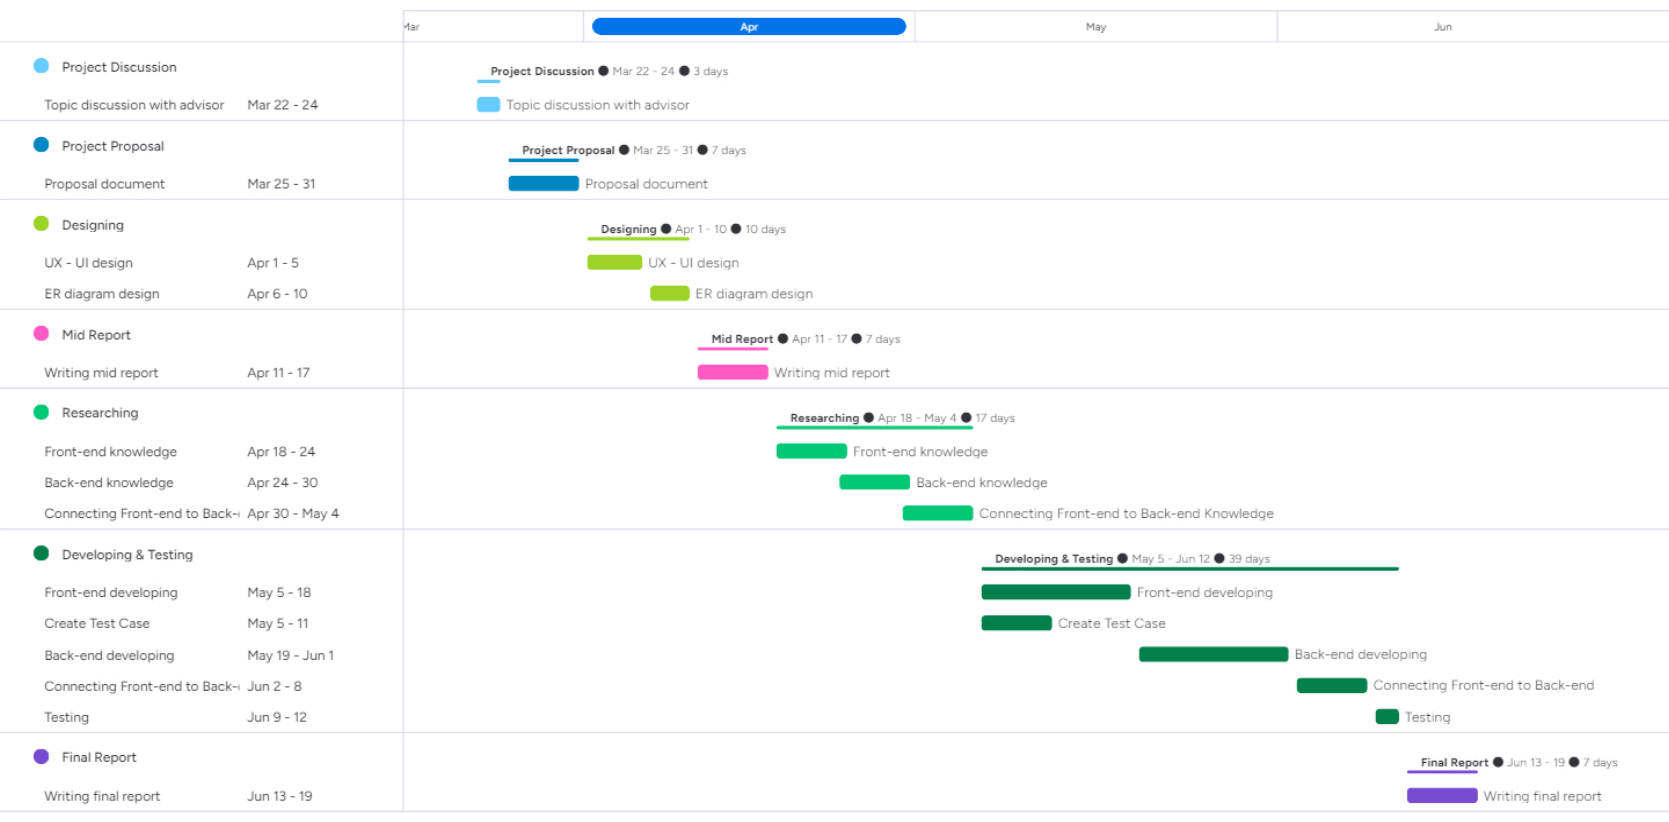
\includegraphics[width=\textwidth, keepaspectratio=true]{image/chap1/gantt.png}}
	\caption{ตารางการดำเนินงานภาคการศึกษาที่ 1}\label{fig:plan}
\end{figure}

\section{ผลการดำเนินงาน}

\begin{itemize}
	\item รายงานรูปเล่มฉบับสมบูรณ์
	\item การออกแบบ
	      \begin{itemize}
		      \item รายละเอียดของระบบ
		      \item โครงสร้างสถาปัตยกรรมระบบ
		      \item แบบจำลองหน้าจอส่วนต่อประสานกับผู้ใช้
		      \item โครงสร้างฐานข้อมูล
		      \item แผนภาพความสามารถของระบบ และแผนภาพการทำงานของระบบ
	      \end{itemize}
	\item ระบบ Front-end
	\item ระบบ Back-end
	\item ข้อมูลคำศัพท์ในฐานข้อมูลเริ่มต้นจำนวน 100 คำ ที่สามารถเพิ่มเติมได้ในภายหลัง
\end{itemize}

%%%%%%%%%%%%%%%%%%%%%%%%%%%%%%%%%%%%%%%%%%%%%%%%%%%%%%%%%%%%%%%
%%%%%%%%%%%%%%%%%%%%%%%%%% Chapter 2 %%%%%%%%%%%%%%%%%%%%%%%%%%
%%%%%%%%%%%%%%%%%%%%%%%%%%%%%%%%%%%%%%%%%%%%%%%%%%%%%%%%%%%%%%%

\chapter{ทฤษฎีและงานวิจัยที่เกี่ยวข้อง}

%%%%%%%%%%%%%%%%%%%%%%%%%% 2.1 %%%%%%%%%%%%%%%%%%%%%%%%%%

\section{ทฤษฎีที่เกี่ยวข้อง}

\hspace{1cm}
หัวข้อนี้จะพูดเกี่ยวกับทฤษฎีที่เกี่ยวข้องกับโครงงาน โดยหัวข้อที่เกี่ยวข้องคือวิธีการเรียนรู้คำศัพท์
คือการใช้บัตรคำในการจำศัพท์ และข้อสอบแบบเลือกตอบสำหรับการวัดผล และวิธีการเรียนรู้รูปแบบต่าง ๆ
ที่นำมาปรับใช้ในโครงงาน คือ Computer-Aided Instruction ซึ่งเป็นการนำคอมพิวเตอร์มาปรับใช้กับการเรียนรู้
และ Games-Based Learning ซึ่งเป็นการนำเกมมาใช้เป็นสื่อการสอน

\subsection{การเรียนรู้คำศัพท์}

\hspace{1cm}
การเรียนรู้คำศัพท์ คือ กระบวนการเรียนรู้คำศัพท์ โดยใช้ความรู้ ความจำ และความเข้าใจในความหมาย ความหมายของคำ
การสะกด การออกเสียง และของคำศัพท์ใหม่ ๆ อีกทั้งยังรวมถึงการนำคำศัพท์ที่เรียนรู้มาไปใช้ในบริบทต่าง ๆ ได้อยากถูกต้อง

\subsection{บัตรคำ}

\hspace{1cm}
บัตรคำ (Flash card) เป็นสื่อการสอนในรูปแบบหนึ่ง โดยด้านหนึ่งจะประกอบไปด้วยคำศัพท์
และอีกด้านจะเป็นความหมายหรือรูปภาพของคำศัพท์นั้น ๆ ซึ่งจะช่วยกระตุ้นทักษะในด้านการจดจำคำศัพท์
เนื่องจากเป็นการทำอะไรซ้ำ ๆ และทำให้เรียนรู้คำศัพท์ใหม่ ๆ ได้เยอะขึ้น

\subsection{ข้อสอบแบบเลือกตอบ}

\hspace{1cm}
ข้อสอบแบบเลือกตอบ (Multiple choice question) เป็นเครื่องมือการวัดผลชนิดหนึ่งที่มีลักษณะสำคัญคือ
เป็นคำถามและมีตัวเลือกหลายตัวเลือกให้ผู้สอบเลือกตอบข้อที่ถูกเพียงข้อเดียว จะใช้วัดผลด้านความรู้เป็นหลัก
และสามารถตรวจให้คะแนนได้เหมือนกันแม้จะเป็นผู้ตรวจคนละคนกัน อีกทั้งยังสามารถประเมิณความรู้ได้ทั้งในระดับของความจำ
และการประยุกต์ใช้ความรู้ แต่ทั้งนี้ในการจะวัดความรู้ได้ดีหรือไม่ก็ขึ้นอยู่กับการสร้างคำถาม

\subsection{Games-Based Learning \cite{GBL}}

\hspace{1cm}
Games-based learning คือการเรียนรู้โดยใช้เกมมาผสมผสาน ซึ่งจะทำให้เกิดการเรียนรู้ไปพร้อมกับได้รับความสนุกจากเกม
โดยเกิดจากการที่นักวิจัยด้านการศึกษาได้นำเสนอแนวคิดที่จะนำความบันเทิงเข้ามาเป็นส่วนหนึ่งกับการเรียนรู้ และเมื่อการเรียนมีความสนุกสนาน
ก็จะช่วยให้ผู้เรียนมีความสนใจในการเรียนรู้มากขึ้น และทำให้เกิดการเรียนรู้ได้เร็วยิ่งขึ้น ต่างจากการเรียนปกติที่อาจทำให้เกิดความเคร่งเครียด
และนำไปสู่การไม่สนใจในการเรียนรู้ และละเลยการศึกษา

\subsection{Computer-Aided Instruction \cite{CAI1,CAI2}}

\hspace{1cm}
Computer-Aided Instruction คือสื่อการเรียนรู้รูปแบบหนึ่ง ที่ใช้ความสามารถของคอมพิวเตอร์นำเสนอสื่อ และข้อมูลต่าง ๆ
ไม่ว่าจะเป็นข้อความ ภาพ หรือเสียง โดยมีลักษณะการเรียนแบบที่ผู้เรียนมีการโต้ตอบโดยตรงกับคอมพิวเตอร์
ซึ่งจะช่วยดึงดูดความสนใจของผู้เรียน และสร้างแรงจูงใจในการเรียนรู้มากขึ้น

%%%%%%%%%%%%%%%%%%%%%%%%%% 2.2 %%%%%%%%%%%%%%%%%%%%%%%%%%

\section{ภาษาคอมพิวเตอร์และเทคโนโลยี}

\hspace{1cm}
หัวข้อนี้จะพูดถึงภาษาคอมพิวเตอร์และเทคโนโลยีที่ใช้ในโครงงาน ประกอบไปด้วย React
ซึ่งใช้พัฒนา Frontend, Django ใช้พัฒนา Backend และ Figma ที่ใช้ออกแบบ User Interface

\subsection{React}

\hspace{1cm}
React เป็น JavaScript Library ที่ใช้สำหรับสร้าง User interface โดยมีความสามารถในการแบ่ง UI ที่มีความซับซ้อนให้เป็นส่วนเล็ก ๆ ได้
ซึ่งแต่ละส่วนสามารถแยกการทำงานออกจากกันได้อย่างอิสระ และสามารถนำแต่ละส่วนกลับมาใช้ได้อีก ซึ่งทำให้ง่ายต่อการจัดการและแก้ไขโค้ด

\subsection{Django}

\hspace{1cm}
Django เป็น Web framework สำหรับการสร้างเว็บแอปพลิเคชันโดยใช้ภาษา Python ซึ่งมี Architectural pattern
แบบ Model-View-Controller (MVC) และมีคุณสมบัติหลากหลาย เช่น มีระบบแอดมินที่สามารถใช้งานได้ทันที
มี Object-Relational Mapping (ORM) ที่ช่วยให้เชื่อมต่อกับฐานข้อมูลได้อย่างสะดวก และระบบการยืนยันตัวตน (Authentication)
ซึ่งทำให้ง่ายต่อการพัฒนาและปรับปรุงเว็บไซต์ที่ซับซ้อนได้อย่างรวดเร็ว

\subsection{Figma \cite{Figma}}

\hspace{1cm}
Figma เป็นเครื่องมือออกแบบกราฟิกแบบออนไลน์ที่ช่วยให้นักออกแบบสามารถสร้างและออกแบบ UI/UX ของเว็บไซต์
แอปพลิเคชั่น หรือผลิตภัณฑ์อื่น ๆ ได้อย่างง่ายดาย และมีความยืดหยุ่นสูง สามารถใช้งานได้ทั้งบนเว็บและอุปกรณ์เคลื่อนที่
อีกทั้ง Figma ยังได้อันดับ 1 ในการจัดอันดับ UI design tool ประจำปี 2022 ของ uxtool.co อีกด้วย

%%%%%%%%%%%%%%%%%%%%%%%%%% 2.3 %%%%%%%%%%%%%%%%%%%%%%%%%%
\pagebreak
\section{งานวิจัยที่เกี่ยวข้อง}

\hspace{1cm}
หัวข้อนี้จะพูดถึงงานวิจัยที่เกี่ยวข้อกับโครงงาน โดยจะเป็นแอปพลิเคชันที่เกี่ยวข้องกับการเรียนภาษาอังกฤษ
ประกอบไปด้วย Duocards, Memrise และ Duolingo

\subsection{DuoCards  \cite{DuoCards}}

% \begin{figure}[!h]\centering
%   
\includegraphics[width=0.2\textwidth, keepaspectratio=true]{image/chap2/duocards.png}
%   \caption{Icon ของ Duocards}\label{fig:duocardsIcon}
% \end{figure}

\hspace{1cm}
DuoCards เป็นแอปพลิชันที่ออกแบบมาเพื่อช่วยให้ผู้ใช้สามารถเรียนรู้และจดจำคำศัพท์ ใหม่ ๆ ในหลายภาษาโดยใช้บัตรคำ
โดยผู้ใช้สามารถใช้ชุดคำศัพท์ที่มีการเตรียมไว้ให้ หรือสร้างและออกแบบบัตรคำของตัวเองได้

\begin{figure}[!h]\centering
	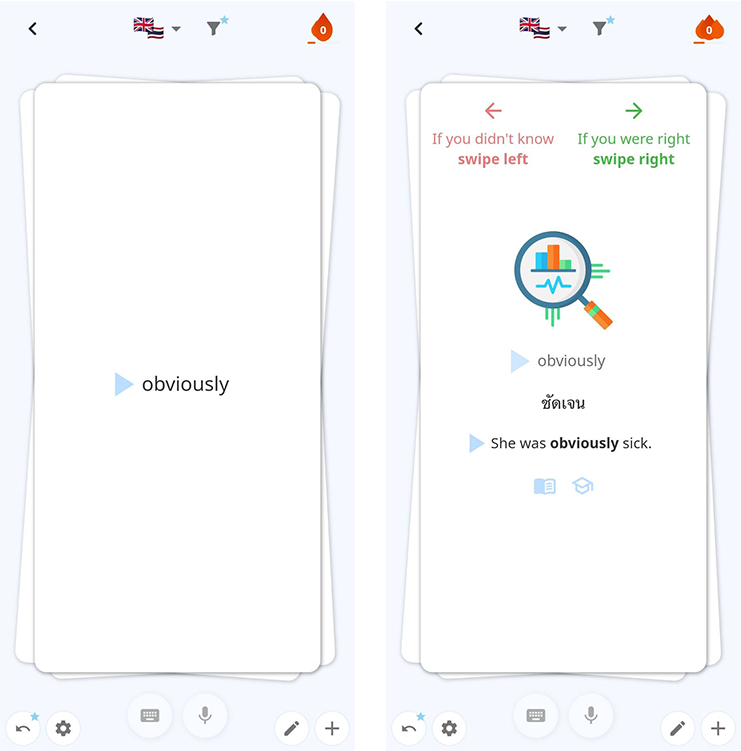
\includegraphics[width=0.8\textwidth, keepaspectratio=true]{image/chap2/duocardsEX.png}
	\caption{แอปพลิเคชัน Duocards}\label{fig:duocardsEx}
\end{figure}

\begin{itemize}
	\item ข้อดี
	      \begin{enumerate}
		      \item มีคอร์สเรียนและแบบฝึกหัดในหลากหลายภาษา
		      \item สามารถสร้างชุดคำศัพท์ของตัวเองได้
		      \item สามารถเรียนรู้คำศัพท์จากวิดีโอที่แอปพลิเคชันเตรียมไว้ให้ได้
		      \item มีการเรียนรู้ในรูปแบบเกมที่มีรางวัลและความสำเร็จเพื่อเป็นแรงจูงใจให้ผู้ใช้
		      \item มีชุมชนสำหรับผู้ใช้เพื่อการแข่งขันและแลกเปลี่ยนข้อมูล
	      \end{enumerate}
	\item ข้อเสีย
	      \begin{enumerate}
		      \item มีวิธีการเรียนรู้คำศัพท์ในรูปแบบเดียวเท่านั้นคือบัตรคำ
	      \end{enumerate}
\end{itemize}

\pagebreak
\subsection{Memrise \cite{Memrise}}

\hspace{1cm}
Memrise เป็นแอปพลิเคชันสำหรับการเรียนรู้ภาษาที่มีรูปแบบในการเรียนรู้หลากหลาย ไม่ว่าจะเป็นแบบทดสอบหลายตัวเลือก
หรือการพิมพ์คำศัพท์ให้ถูกต้อง อีกทั้งยังมีภาษาให้เลือกเรียนถึง 22 ภาษา โดยผู้ใช้สามารถสร้างบทเรียนของตัวเองเพื่อแบ่งปันกับผู้ใช้คนอื่นได้อีกด้วย

\begin{figure}[!h]\centering
	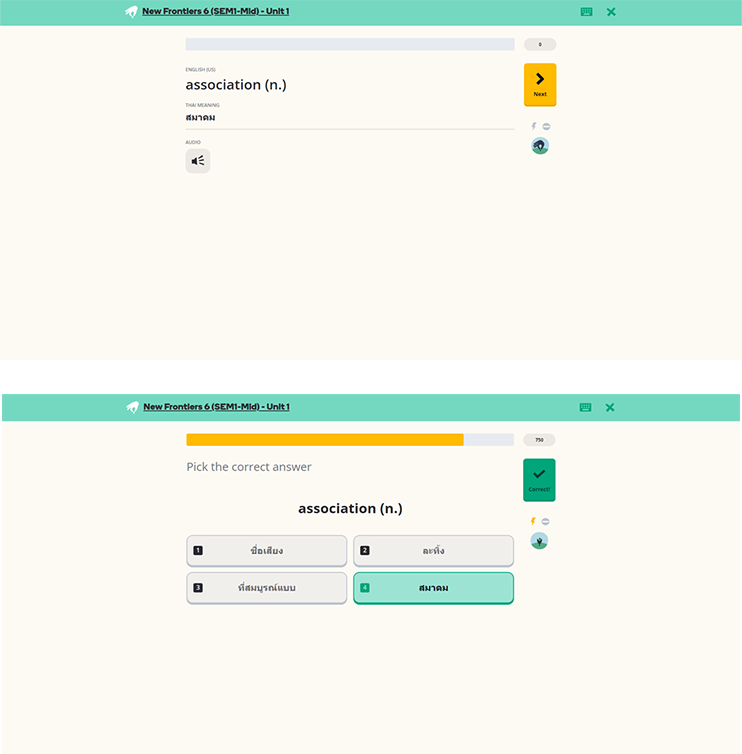
\includegraphics[width=0.8\textwidth, keepaspectratio=true]{image/chap2/memriseEX.png}
	\caption{แอปพลิเคชัน Memrise}\label{fig:mimriseEx}
\end{figure}

\begin{itemize}
	\item ข้อดี
	      \begin{enumerate}
		      \item มีคอร์สเรียนและแบบฝึกหัดในหลายภาษา และยังสามารถเลือกหัวข้อการเรียนที่สนใจได้ เช่นคำศัพท์ทางวิทยาศาสตร์ หรือคำศัพท์ทางธุรกิจ
		      \item สามารถสร้างบทเรียนหรือชุดคำศัพท์ของตนเองเพื่อแบ่งปันกับผู้ใช้งานคนอื่นได้
		      \item มีการเก็บค่าประสบการณ์ และความสำเร็จเพื่อเป็นแรงจูงใจให้ผู้ใช้
		      \item มีชุมชนสำหรับผู้ใช้เพื่อการแข่งขันและแลกเปลี่ยนข้อมูล
	      \end{enumerate}
	\item ข้อเสีย
	      \begin{enumerate}
		      \item การเรียนรู้ส่วนใหญ่ที่มีจะอยู่ในรูปแบบการเลือกคำตอบให้ถูกต้อง
		      \item ไม่สามารถเลือกรูปแบบการเรียนรู้ของบทเรียนที่มีอยู่ ยกเว้นจะทำการสร้างบทเรียนขึ้นมาเอง
	      \end{enumerate}
\end{itemize}

\pagebreak
\subsection{Duolingo \cite{Duolingo}}

\hspace{1cm}
Duolingo เป็นแอปพลิเคชันสำหรับการเรียนรู้ภาษาที่ครอบคลุมถึง 40 ภาษา อีกทั้งยังมีการเรียนรู้ที่ครอบคลุมทั้งการฟัง การพูด การอ่าน และการเขียน
ตัวอย่างเช่นการจับคู่คำศัพท์, แบบทดสอบหลายตัวเลือก, การเรียงประโยคให้ถูกต้อง และการฝึกพูด เป็นต้น ซึ่งทำให้การเรียนรู้มีความสนุกและน่าสนใจมากขึ้น

\begin{figure}[!h]\centering
	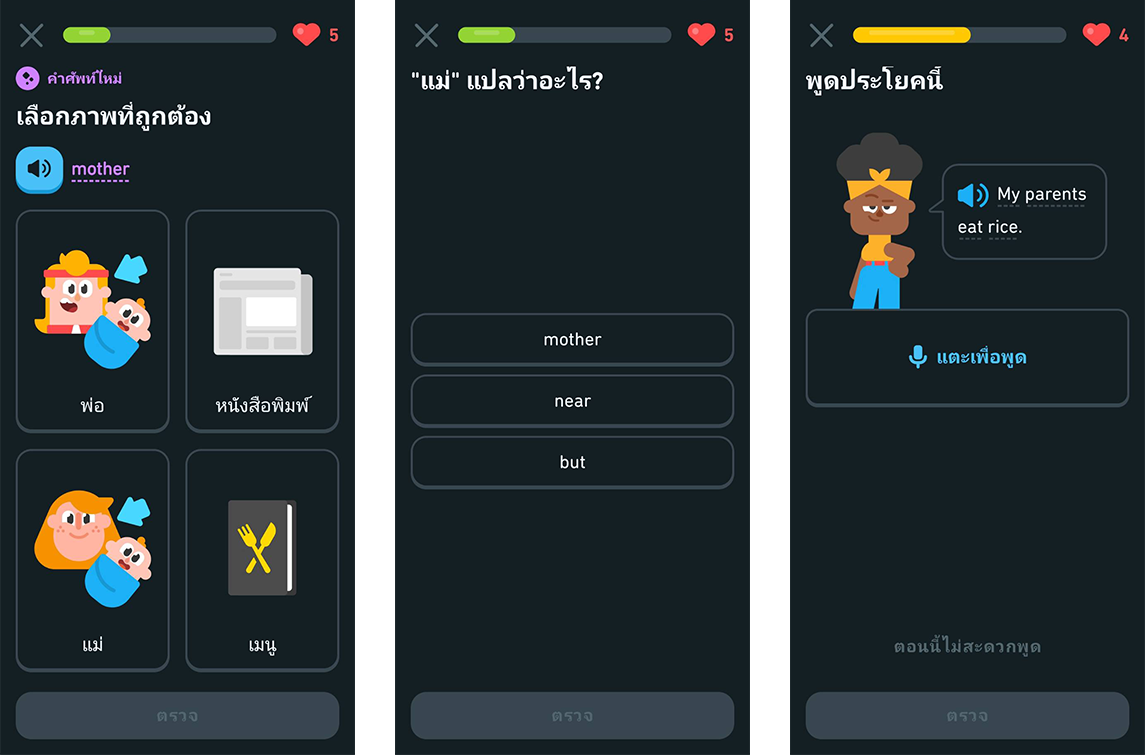
\includegraphics[width=0.8\textwidth, keepaspectratio=true]{image/chap2/duolingoEX.png}
	\caption{แอปพลิเคชัน Duolingo}\label{fig:duolingoEX}
\end{figure}

\begin{itemize}
	\item ข้อดี
	      \begin{enumerate}
		      \item มีคอร์สเรียนและแบบฝึกหัดในหลายภาษา
		      \item มีระบบการเรียนรู้ที่หลากหลาย ทั้งฟัง พูด อ่าน และเขียนสามารถสร้างบทเรียนหรือชุดคำศัพท์ของตนเองเพื่อแบ่งปันกับผู้ใช้งานคนอื่นได้
		      \item มีระบบการเรียนรู้แบบเกมที่มีรางวัลและความสำเร็จที่สามารถให้แรงจูงใจกับผู้ใช้ได้
		      \item มีชุมชนสำหรับผู้ใช้เพื่อการแข่งขันและแลกเปลี่ยนข้อมูล
	      \end{enumerate}
	\item ข้อเสีย
	      \begin{enumerate}
		      \item แอปอาจไม่เหมาะสำหรับผู้ใช้ที่ต้องการเน้นการเรียนรู้คำศัพท์เท่านั้น เนื่องจากแอปถูกออกแบบให้เป็นแพลตฟอร์มการเรียนรู้ภาษาแบบครอบคลุม
		      \item ไม่สามารถเลือกหมวดหมู่ของการเรียนได้ตามต้องการ ต้องเรียนตามบทเรียนที่แอปพลิเคชันสร้างไว้
		      \item ไม่สามารถสร้างบทเรียนของตนเองได้
	      \end{enumerate}
\end{itemize}

%%%%%%%%%%%%%%%%%%%%%%%%%%%%%%%%%%%%%%%%%%%%%%%%%%%%%%%%%%%%%%%
%%%%%%%%%%%%%%%%%%%%%%%%%% Chapter 3 %%%%%%%%%%%%%%%%%%%%%%%%%%
%%%%%%%%%%%%%%%%%%%%%%%%%%%%%%%%%%%%%%%%%%%%%%%%%%%%%%%%%%%%%%%

\chapter{วิธีการทำงาน กระบวนการและการออกแบบ}

\section{รายละเอียดของโครงงาน}
\hspace{1cm}
หัวข้อนี้จะพูดถึงรายละเอียดต่าง ๆ ที่โครงงานสามารถทำได้ โดยจะประกอบไปด้วยความต้องการระบบ
ซึ่งเป็นความต้องการพื้นฐาน และคุณสมบัติต่าง ๆ ของระบบ รวมถึง Use Case Diagram
และ Use Case Narrative ซึ่งจะแสดงให้เห็นถึงสิ่งที่ระบบสามารถทำได้

\subsection{ความต้องการระบบ}
\begin{itemize}
	\item สามารถเข้าถึงได้ผ่านทุกเว็บเบราเซอร์บนคอมพิวเตอร์
	\item ฐานข้อมูลคำศัพท์โดยเป็นคำศัพท์ภาษาอังกฤษที่สามารถค้นหาได้ พร้อมความหมายทั้งภาษาไทยและภาษาอังกฤษ ตัวอย่างการใช้งานในประโยค และวิธีการออกเสียง
	\item สามารถสุ่มคำศัพท์ภาษาอังกฤษใหม่ ๆ ที่ยังไม่เคยเรียน พร้อมความหมายทั้งภาษาไทย ภาษาอังกฤษ ตัวอย่างการใช้งานในประโยค และวิธีการออกเสียง
	\item สามารถสร้างบัตรคำ ซึ่งเป็นบัตรที่ประกอบไปด้วยคำศัพท์ภาษาอังกฤษ และความหมายภาษาไทยได้ โดยผู้ใช้สามารถเลือกคำศัพท์แล้วบันทึกไว้เอง หรือจะเลือกจากที่ระบบจัดไว้ให้
	\item สามารถทดสอบความรู้ด้วยแบบทดสอบหลายตัวเลือกได้ โดยผู้ใช้จะต้องทำการจับคู่คำศัพท์กับความหมายให้ถูกต้อง
	\item สามารถเล่นเกมเรียงตัวอักษรให้ถูกต้องได้ โดยระบบจะทำการสลับตำแหน่งตัวอักษร และให้คำใบ้มา ผู้ใช้จะต้องทำการพิมพ์คำศัพท์ที่ถูกต้อง
	\item สามารถติดตามความคืบหน้าได้ โดยมีจำนวนคำศัพท์ที่เรียนไป จำนวนเกมที่เล่นจบ และเวลาที่ใช้ไปในแอปพลิเคชัน
\end{itemize}

\pagebreak
\subsection{Use Case Diagram}

\begin{figure}[!h]\centering
	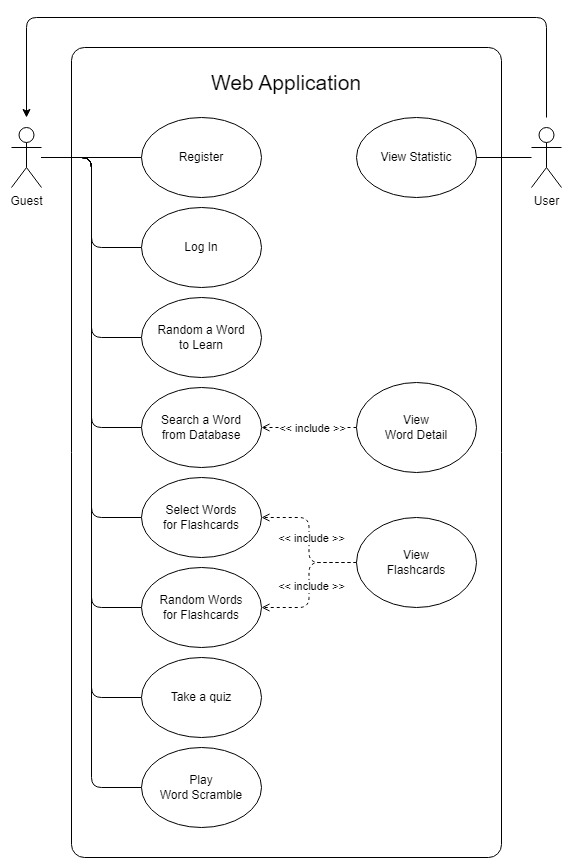
\includegraphics[width=0.8\textwidth, keepaspectratio=true]{image/chap3/UseCaseDiagram.jpg}
	\caption{แผนภาพที่แสดงการทำงานของระบบ}\label{fig:UseCaseDiagram}
\end{figure}

\hspace{1cm}
จากภาพจะเห็นว่าประกอบด้วย 2 บทบาทคือ Guest และ User โดยแต่ละบทบาทมีหน้าที่ดังนี้
\begin{itemize}
	\item Guest คือผู้ใช้ทั่วไปที่ยังไม่ได้ลงทะเบียนผู้ใช้ในระบบ หรือยังไม่ได้เข้าสู่ระบบ
	      โดยสามารถลงทะเบียนผู้ใช้งาน เข้าสู่ระบบ สุ่มคำศัพท์ ค้นหาคำศัพท์ แสดงรายละเอียดคำศัพท์ที่ค้นหา
	      เลือกหรือสุ่มคำศัพท์เพื่อใช้งานบัตรคำ ดูบัตรคำ ทำแบบทดสอบ และเล่นเกม
	\item User คือผู้ใช้ที่เข้าสู่ระบบแล้ว สามารถดูสถิติการใช้งานเว็บแอปพลิชันได้
\end{itemize}

\subsection{Use Case Narrative}
ประกอบด้วย 11 Use Cases ดังรูปภาพที่ \ref{fig:UseCaseDiagram} โดยมีรายละเอียดดังนี้

\subsubsection{ลงทะเบียนผู้ใช้งาน}
\begin{table}[h]\centering
	\caption{คำอธิบาย Use Case สำหรับการลงทะเบียนผู้ใช้งาน}\label{tbl:U_Register}
	\begin{tabular}{|p{.2\linewidth}|p{.6\linewidth}|}
		\hline
		Use Case Name:         & Register                                                                                                                                                                                           \\ \hline
		Actor:                 & Guest                                                                                                                                                                                              \\ \hline
		Goal:                  & ลงทะเบียนผู้ใช้งานสำเร็จ                                                                                                                                                                                 \\ \hline
		Precondition           & Guest เข้าหน้า Register/Log In                                                                                                                                                                       \\ \hline
		Main Success Scenario: & \begin{tabular}[c]{@{}l@{}}1. ระบบร้องขอการกรอกข้อมูล \\2. Guest กรอกข้อมูล \\3. ระบบถามการยืนยันข้อมูล \\4. Guest ยืนยันข้อมูล \\5. ระบบสร้าง Account ให้กับ Guest\end{tabular}                                   \\ \hline
		Postcondition          & Guest มีบัญชีในระบบ                                                                                                                                                                                   \\ \hline
		Extention              & \begin{tabular}[c]{@{}l@{}}Extension (a) \\ 4a. Guest กดยกเลิก \\ 5a. กลับไปทำข้อ 2. \\ 2. Extension (b) \\ 3b. Admin กรอกข้อมูลไม่ตรงตามรูปแบบ \\ 4b. ระบบแจ้งเตือนข้อผิดพลาด \\ 5b. กลับไปทำข้อ 1.\end{tabular} \\ \hline
	\end{tabular}
\end{table}

\subsubsection{เข้าสู่ระบบ}
\begin{table}[h]\centering
	\caption{คำอธิบาย Use Case สำหรับการเข้าสู่ระบบ}\label{tbl:U_LogIn}
	\begin{tabular}{|p{.2\linewidth}|p{.6\linewidth}|}
		\hline
		Use Case Name:         & Log In                                                                                                                              \\ \hline
		Actor:                 & Guest                                                                                                                               \\ \hline
		Goal:                  & เข้าสู่ระบบสำเร็จ                                                                                                                        \\ \hline
		Precondition           & Guest เข้าหน้า Register/Log In                                                                                                        \\ \hline
		Main Success Scenario: & \begin{tabular}[c]{@{}l@{}}1. Actor กรอก Username และ Password \\2. Actor กดยืนยัน \\3. ระบบยืนยันให้เข้าสู่ระบบ \end{tabular}              \\ \hline
		Extention              & \begin{tabular}[c]{@{}l@{}}Extension (a) \\ 3a. ข้อมูลที่Actor กรอกมาไม่ถูกต้อง \\ 4a. ระบบแจ้งเตือนข้อผิดพลาด \\ 5a. กลับไปทำข้อ 1.\end{tabular} \\ \hline
	\end{tabular}
\end{table}

\pagebreak
\subsubsection{ดูสถิติการใช้งานเว็บแอปพลิเคชัน}
\begin{table}[h]\centering
	\caption{คำอธิบาย Use Case สำหรับการดูสถิติการใช้งานเว็บแอปพลิเคชัน}\label{tbl:U_Statistic}
	\begin{tabular}{|p{.2\linewidth}|p{.6\linewidth}|}
		\hline
		Use Case Name:         & View Statistic                                                                                 \\ \hline
		Actor:                 & User                                                                                           \\ \hline
		Goal:                  & ดูสถิติการใช้งานสำเร็จ                                                                               \\ \hline
		Precondition           & User ทำการ Log-in เข้ามาแล้ว, User กดที่ไอคอนผู้ใช้งาน                                                 \\ \hline
		Main Success Scenario: & \begin{tabular}[c]{@{}l@{}}1. User เลือกดูสถิติ \\2. ระบบแสดงสถิติการใช้งานเว็บแอปพลิเคชัน \end{tabular} \\ \hline
	\end{tabular}
\end{table}

\subsubsection{สุ่มคำศัพท์ใหม่เพื่อการเรียนรู้}
\begin{table}[h]\centering
	\caption{คำอธิบาย Use Case สำหรับการสุ่มคำศัพท์ใหม่เพื่อการเรียนรู้}\label{tbl:U_RandomWord}
	\begin{tabular}{|p{.2\linewidth}|p{.6\linewidth}|}
		\hline
		Use Case Name:         & Random a Word to Learn                                                                    \\ \hline
		Actor:                 & Guest, User                                                                               \\ \hline
		Goal:                  & ระบบแสดงคำศัพท์ที่สุ่มมาสำเร็จ                                                                     \\ \hline
		Precondition           & Actor อยู่หน้า Homepage                                                                      \\ \hline
		Main Success Scenario: & \begin{tabular}[c]{@{}l@{}}1. Actor เลือก Random Word \\2. ระบบแสดงคำศัพท์ที่สุ่มมา \end{tabular} \\ \hline
	\end{tabular}
\end{table}

\subsubsection{ค้นหาคำศัพท์จากฐานข้อมูล}
\begin{table}[h]\centering
	\caption{คำอธิบาย Use Case สำหรับการค้นหาคำศัพท์จากฐานข้อมูล}\label{tbl:U_SearchWord}
	\begin{tabular}{|p{.2\linewidth}|p{.6\linewidth}|}
		\hline
		Use Case Name:         & Search a Word from Database                                                                                                      \\ \hline
		Actor:                 & Guest, User                                                                                                                      \\ \hline
		Goal:                  & แสดงคำศัพท์ที่ค้นหาสำเร็จ                                                                                                                \\ \hline
		Precondition           & Actor อยู่หน้า Homepage หรือ Actor อยู่หน้า Dictionary                                                                                  \\ \hline
		Main Success Scenario: & \begin{tabular}[c]{@{}l@{}}1. Actor กรอกคำศัพท์ที่ต้องการค้นหา \\2. Actor กดค้นหา \\3. ระบบแสดงคำศัพท์ที่ค้นหา \end{tabular}                   \\ \hline
		Extention              & \begin{tabular}[c]{@{}l@{}}Extension (a) \\ 3a. ระบบไม่มีคำศัพท์ที่ Actor ค้นหา \\ 4a. ระบบแสดงว่าไม่มีคำศัพท์ \\ 5a. กลับไปทำข้อ 1.\end{tabular} \\ \hline
	\end{tabular}
\end{table}

\pagebreak
\subsubsection{แสดงผลรายละเอียดคำศัพท์}
\begin{table}[h]\centering
	\caption{คำอธิบาย Use Case สำหรับการแสดงผลรายละเอียดคำศัพท์}\label{tbl:U_WordDetail}
	\begin{tabular}{|p{.2\linewidth}|p{.6\linewidth}|}
		\hline
		Use Case Name:         & View Word Detail                                                                                  \\ \hline
		Actor:                 & Guest, User                                                                                       \\ \hline
		Goal:                  & แสดงผลรายละเอียดคำศัพท์สำเร็จ                                                                           \\ \hline
		Precondition           & Actor ค้นหาคำศัพท์                                                                                    \\ \hline
		Main Success Scenario: & \begin{tabular}[c]{@{}l@{}}1. Actor กดปุ่มดูรายละเอียดคำศัพท์ \\2. ระบบแสดงผลรายละเอียดคำศัพท์ \end{tabular} \\ \hline
	\end{tabular}
\end{table}

\subsubsection{เลือกคำศัพท์เพื่อใช้งานบัตรคำ}
\begin{table}[h]\centering
	\caption{คำอธิบาย Use Case สำหรับการเลือกคำศัพท์เพื่อใช้งานบัตรคำ}\label{tbl:U_RandomFlashCard}
	\begin{tabular}{|p{.2\linewidth}|p{.6\linewidth}|}
		\hline
		Use Case Name:         & Select Words for Flashcards                                                                                                                                 \\ \hline
		Actor:                 & Guest, User                                                                                                                                                 \\ \hline
		Goal:                  & เลือกคำศัพท์สำเร็จ                                                                                                                                                \\ \hline
		Precondition           & Actor เลือก Select Word ในหน้า Flashcard                                                                                                                      \\ \hline
		Main Success Scenario: & \begin{tabular}[c]{@{}l@{}}1. ระบบแสดงคำศัพท์ \\2. Actor เลือกเก็บคำศัพท์นั้นเพื่อใช้งานบัตรคำ \\3. ระบบเก็บคำศัพท์ที่เลือก \\4. กลับไปทำข้อที่ 1. จนระบบเก็บคำศัพท์ครบ 10 คำ \end{tabular} \\ \hline
		Postcondition          & ระบบมีคำศัพท์เพื่อใช้แสดงบัตรคำ                                                                                                                                      \\ \hline
		Extention              & \begin{tabular}[c]{@{}l@{}}Extension (a) \\ 2a. Actor เลือกทิ้งคำศัพท์ \\ 3a. กลับไปทำข้อ 1. จนระบบเก็บคำศัพท์ครบ 10 คำ\end{tabular}                                      \\ \hline
	\end{tabular}
\end{table}

\subsubsection{สุ่มคำศัพท์เพื่อใช้งานบัตรคำ}
\begin{table}[h]\centering
	\caption{คำอธิบาย Use Case สำหรับการสุ่มคำศัพท์เพื่อใช้งานบัตรคำ}\label{tbl:U_SelectFlashcard}
	\begin{tabular}{|p{.2\linewidth}|p{.6\linewidth}|}
		\hline
		Use Case Name:         & Random Words for Flashcards                                                                            \\ \hline
		Actor:                 & Guest, User                                                                                            \\ \hline
		Goal:                  & สุ่มคำศัพท์สำเร็จ                                                                                             \\ \hline
		Precondition           & Actor เลือก Random Word ในหน้า Flashcard                                                                 \\ \hline
		Main Success Scenario: & \begin{tabular}[c]{@{}l@{}}1. ระบบสุ่มคำศัพท์มาจำนวน 10 คำ  \\2. ระบบเก็บคำศัพท์ทั้ง 10 คำ เพื่อใช้งานบัตรคำ\end{tabular} \\ \hline
		Postcondition          & ระบบมีคำศัพท์เพื่อใช้แสดงบัตรคำ                                                                                 \\ \hline
	\end{tabular}
\end{table}

\pagebreak
\subsubsection{ดูบัตรคำ}
\begin{table}[h]\centering
	\caption{คำอธิบาย Use Case สำหรับการดูบัตรคำ}\label{tbl:U_Flashcard}
	\begin{tabular}{|p{.2\linewidth}|p{.6\linewidth}|}
		\hline
		Use Case Name:         & View Flashcards                                                                                                                                                                                                                                                                                                                                                                                                        \\ \hline
		Actor:                 & Guest, User                                                                                                                                                                                                                                                                                                                                                                                                            \\ \hline
		Goal:                  & Actor กดปุ่มจำคำศัพท์ได้ครบ 10 คำ                                                                                                                                                                                                                                                                                                                                                                                              \\ \hline
		Precondition           & ระบบมีคำศัพท์เพื่อใช้แสดงบัตรคำ                                                                                                                                                                                                                                                                                                                                                                                                 \\ \hline
		Main Success Scenario: & \begin{tabular}[c]{@{}l@{}}1. ระบบแสดงบัตรคำด้านหน้า \\2. Actor กดที่บัตรคำ \\3. ระบบแสดงบัตรคำด้านหลัง \\4. Actor กดปุ่มจำคำศัพท์ได้ \\5. ระบบลบคำศัพท์ออก และแสดงคำศัพท์ถัดไป \\6. กลับไปทำข้อ 1. จน Actor กดปุ่มจำคำศัพท์ได้ครบ 10 คำ \end{tabular}                                                                                                                                                                                                      \\ \hline
		Extention              & \begin{tabular}[c]{@{}l@{}}Extension (a) \\ 2a. Actor กดจำคำศัพท์ได้ \\ 3a. ระบบลบคำศัพท์ออก และแสดงคำศัพท์ถัดไป \\4a. กลับไปทำข้อ 1. จน Actor กดปุ่มจำคำศัพท์ได้ครบ 10 คำ \\Extension (b) \\2b. Actor กดจำคำศัพท์ไม่ได้ \\3b. ระบบเก็บคำศัพท์ไว้ และแสดงคำศัพท์ถัดไป \\4b. กลับไปทำข้อ 1. จน Actor กดปุ่มจำคำศัพท์ได้ครบ 10 คำ \\Extension (c) \\4c. Actor กดจำคำศัพท์ไม่ได้ \\5c. ระบบเก็บคำศัพท์ไว้ และแสดงคำศัพท์ถัดไป \\6c. กลับไปทำข้อ 1. จน Actor กดปุ่มจำคำศัพท์ได้ครบ 10 คำ\end{tabular} \\ \hline
	\end{tabular}
\end{table}

\subsubsection{ทำแบบทดสอบ}
\begin{table}[h]\centering
	\caption{คำอธิบาย Use Case สำหรับการทำแบบทดสอบ}\label{tbl:U_Quiz}
	\begin{tabular}{|p{.2\linewidth}|p{.6\linewidth}|}
		\hline
		Use Case Name:         & Take a quiz                                                                                                                                                                                                     \\ \hline
		Actor:                 & Guest, User                                                                                                                                                                                                     \\ \hline
		Goal:                  & Actor ทำแบบทดสอบครบ 10 คำถาม                                                                                                                                                                                      \\ \hline
		Precondition           & Actor อยู่หน้า Quiz                                                                                                                                                                                                \\ \hline
		Main Success Scenario: & \begin{tabular}[c]{@{}l@{}}1. Actor กด Start \\2. ระบบแสดงคำถามและตัวเลือก \\3. Actor กดปุ่มตัวเลือก \\4. ระบบแสดงผลคำตอบที่ถูกต้อง \\5. กลับไปทำข้อ 2. จน Actor ตอบคำถามครบ 10 ข้อ \\6. ระบบแสดงผลลัพธ์การทำแบบทดสอบ \end{tabular} \\ \hline
	\end{tabular}
\end{table}

\pagebreak
\subsubsection{เล่นเกมเรียงพยัญชนะเป็นคำศัพท์}
\begin{table}[h]\centering
	\caption{คำอธิบาย Use Case สำหรับการเล่นเกมเรียงพยัญชนะเป็นคำศัพท์}\label{tbl:U_Game}
	\begin{tabular}{|p{.2\linewidth}|p{.6\linewidth}|}
		\hline
		Use Case Name:         & Play Word Scramble                                                                                                                                                                                                                                                                                                                                                                                                         \\ \hline
		Actor:                 & Guest, User                                                                                                                                                                                                                                                                                                                                                                                                            \\ \hline
		Goal:                  & Actor เรียงพยัญชนะเป็นคำศัพท์ได้ถูกต้อง                                                                                                                                                                                                                                                                                                                                                                                             \\ \hline
		Precondition           & Actor อยู่หน้า Word Scramble                                                                                                                                                                                                                                                                                                                                                                                                \\ \hline
		Main Success Scenario: & \begin{tabular}[c]{@{}l@{}}1. Actor กด Start \\2. ระบบแสดงหน้าเกม \\3. Actor ใส่พยัญชนะลงไปในกล่องตัวอักษร \\4. Actor ใส่พยัญชนะถูกตำแหน่ง \\5. Actor กด Submit \\6. ระบบแสดงผลพยัญชนะที่อยู่ในตำแหน่งถูกต้อง \\7. ระบบแสดงผลว่าสามารถเรียงคำศัพท์ได้ถูกต้อง \end{tabular}                                                                                                                                                                                                      \\ \hline
		Extention              & \begin{tabular}[c]{@{}l@{}}Extension (a) \\ 4a. Actor ใส่พยัญชนะผิดตำแหน่ง \\ 5a. Actor กด Submit \\6a. ระบบแสดงผลพยัญชนะที่อยู่ในตำแหน่งถูก และผิด \\7a. กลับไปทำข้อ 3\end{tabular} \\ \hline
	\end{tabular}
\end{table}

\pagebreak
\subsection{System Architecture}

\begin{figure}[!h]\centering
	\fbox{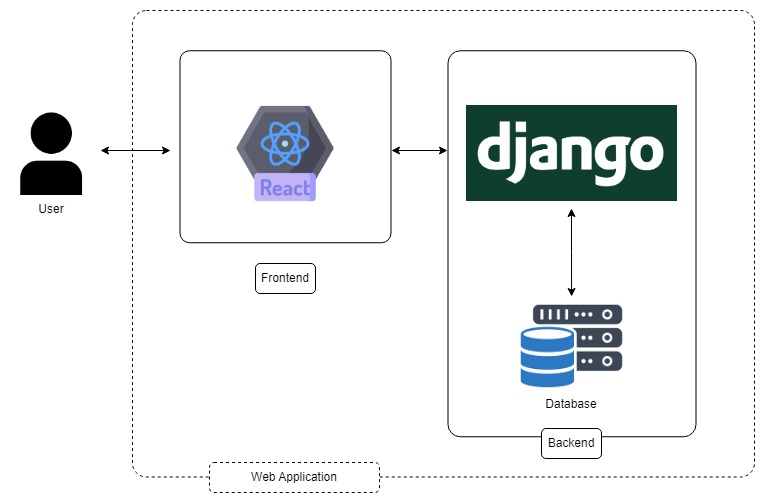
\includegraphics[width=\textwidth, keepaspectratio=true]{image/chap3/System Architecture.jpg}}
	\caption{แผนภาพที่แสดงสถาปัตยกรรมระบบ}\label{fig:UseCaseDiagram}
\end{figure}

\hspace{1cm}
  ในเว็บแอปพลิเคชันจะแบ่งเป็นสองส่วนใหญ่ ๆ คือ Frontend และ Backend โดยผู้ใช้จะติดต่อกับเว็บแอปพลิเคชันผ่านทาง
Frontend ที่พัฒนาโดยใช้ React.js และ Frontend จะติดต่อกับ Backend ที่พัฒนาโดยใช้ Django และ Django
จะรับหน้าที่ในการติดต่อกับฐานข้อมูล

\pagebreak
\subsection{Sequence Diagram}

\subsubsection{ลงทะเบียนผู้ใช้งาน}
\hspace{1cm}
เมื่อผู้ใช้กดปุ่ม Log In แล้ว UI จะร้องขอข้อมูลการลงทะเบียน เมื่อผู้ใช้ส่งข้อมูล UI จะส่งข้อมูลไปที่ Application
เพื่อเพิ่มผู้ใช้ใหม่ และ Application ก็จะเพิ่มข้อมูลลงไปในฐานข้อมูล จากนั้นจึงส่งข้อมูลว่าลงทะเบียนสำเร็จ
และ UI จะแสดงผลว่าลงทะเบียนสำเร็จ
\begin{figure}[!h]\centering
	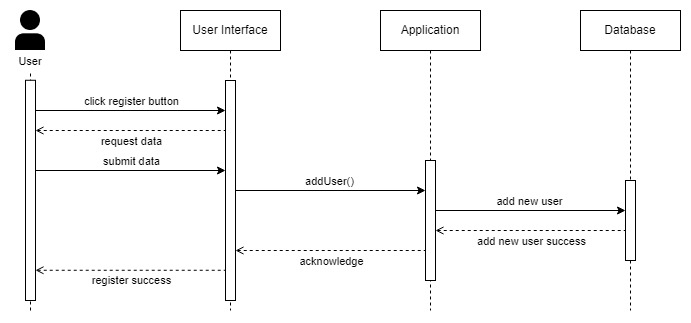
\includegraphics[width=\textwidth, keepaspectratio=true]{image/chap3/sequence/Register.jpg}
	\caption{แผนผังการทำงานแบบลำดับปฏิสัมพันธ์ของการลงทะเบียนผู้ใช้งาน}\label{fig:S_Register}
\end{figure}

\subsubsection{เข้าสู่ระบบ}
\hspace{1cm}
เมื่อผู้ใช้กดปุ่ม Log In แล้ว UI จะร้องขอข้อมูลการเข้าสู่ระบบ เมื่อผู้ใช้ส่งข้อมูล UI จะส่งข้อมูลไปที่ Application
เพื่อเข้าสู่ระบบ และ Application ก็จะเช็คความถูกต้องกับฐานข้อมูล จากนั้นจึงส่งข้อมูลว่าเข้าสู่ระบบสำเร็จ
และ UI จะแสดงผลว่าเข้าสู่ระบบสำเร็จ
\begin{figure}[!h]\centering
	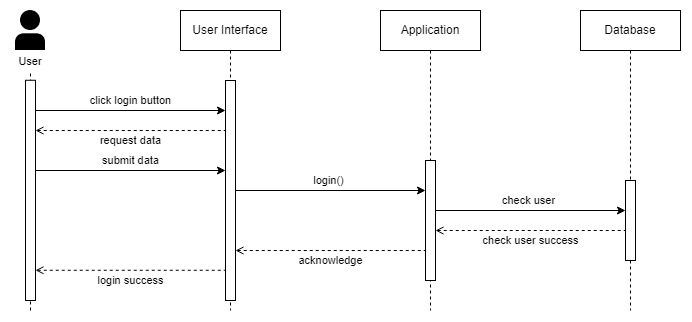
\includegraphics[width=\textwidth, keepaspectratio=true]{image/chap3/sequence/Login.jpg}
	\caption{แผนผังการทำงานแบบลำดับปฏิสัมพันธ์ของการเข้าสู่ระบบ}\label{fig:S_LogIn}
\end{figure}

\pagebreak
\subsubsection{ดูสถิติการใช้งานเว็บแอปพลิเคชัน}
\hspace{1cm}
เมื่อผู้ใช้กดปุ่มดูสถิติการใช้งานเว็บแอปพลิเคชัน UI จะร้องขอข้อมูลสถิติจากฐานข้อมูลผ่าน Application
และฐานข้อมูลจะส่งข้อมูลกลับมาให้ UI เพื่อแสดงผลสถิติการใช้งาน
\begin{figure}[!h]\centering
	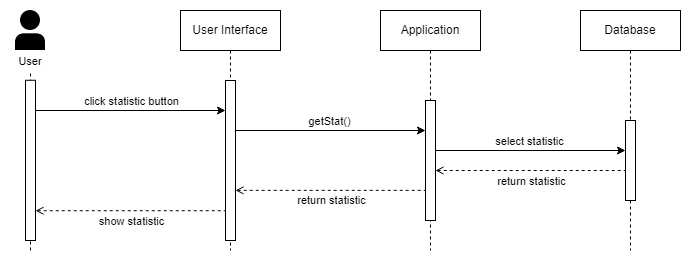
\includegraphics[width=\textwidth, keepaspectratio=true]{image/chap3/sequence/Statistic.jpg}
	\caption{แผนผังการทำงานแบบลำดับปฏิสัมพันธ์ของการดูสถิติการใช้งานเว็บแอปพลิเคชัน}\label{fig:S_Statistic}
\end{figure}

\subsubsection{สุ่มคำศัพท์ใหม่เพื่อการเรียนรู้}
\hspace{1cm}
เมื่อผู้ใช้กดปุ่มสุ่มคำศัพท์ UI จะสุ่มคำศัพท์และร้องข้อมูลคำศัพท์จากฐานข้อมูลผ่าน Application
และฐานข้อมูลจะส่งข้อมูลกลับมาให้ UI เพื่อแสดงผลคำศัพท์ที่สุ่มมา
\begin{figure}[!h]\centering
	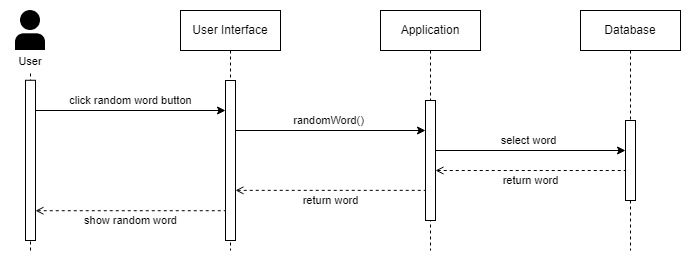
\includegraphics[width=\textwidth, keepaspectratio=true]{image/chap3/sequence/Random word.jpg}
	\caption{แผนผังการทำงานแบบลำดับปฏิสัมพันธ์ของการสุ่มคำศัพท์ใหม่เพื่อการเรียนรู้}\label{fig:S_RandomWord}
\end{figure}

\pagebreak
\subsubsection{ค้นหาคำศัพท์จากฐานข้อมูล}
\hspace{1cm}
เมื่อผู้ใช้กดปุ่มค้นหาคำศัพท์ UI จะร้องข้อมูลคำศัพท์ที่ต้องกับคำค้นหาจากฐานข้อมูลผ่าน Application 
และฐานข้อมูลจะส่งข้อมูลกลับมาให้ UI เพื่อแสดงผลคำศัพท์ที่ค้นหา
\begin{figure}[!h]\centering
	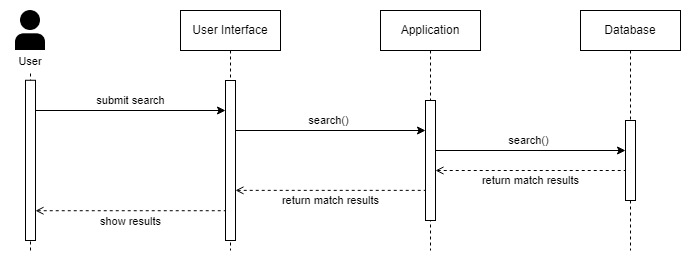
\includegraphics[width=\textwidth, keepaspectratio=true]{image/chap3/sequence/Search.jpg}
	\caption{แผนผังการทำงานแบบลำดับปฏิสัมพันธ์ของการค้นหาคำศัพท์จากฐานข้อมูล}\label{fig:S_SearchWord}
\end{figure}

\subsubsection{แสดงผลรายละเอียดคำศัพท์}
\hspace{1cm}
เมื่อผู้ใช้กดปุ่มแสดงผลรายละเอียดคำศัพท์ UI จะร้องข้อมูลคำศัพท์ดังกล่าวจากฐานข้อมูลผ่าน Application 
และฐานข้อมูลจะส่งข้อมูลกลับมาให้ UI เพื่อแสดงผลรายละเอียดคำศัพท์ที่ผู้ใช้กด
\begin{figure}[!h]\centering
	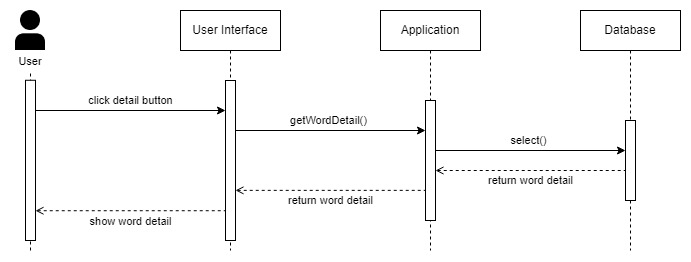
\includegraphics[width=\textwidth, keepaspectratio=true]{image/chap3/sequence/View-Search.jpg}
	\caption{แผนผังการทำงานแบบลำดับปฏิสัมพันธ์ของการแสดงผลรายละเอียดคำศัพท์}\label{fig:S_WordDetail}
\end{figure}

\pagebreak
\subsubsection{เลือกคำศัพท์เพื่อใช้งานบัตรคำ}
\hspace{1cm}
เมื่อผู้ใช้กดปุ่มเลือกคำศัพท์เพื่อใช้งานบัตรคำ UI จะสุ่มคำศัพท์และร้องข้อมูลคำศัพท์จากฐานข้อมูลผ่าน Application 
และฐานข้อมูลจะส่งข้อมูลกลับมาให้ UI เพื่อแสดงผลคำศัพท์ดังกล่าว และเมื่อผู้ใช้ทำการเลือกคำศัพท์นั้นเพื่อใช้งานบัตรคำ 
UI จะส่งข้อมูลดังกล่าวไปเก็บไว้ที่ Application จากนั้นจะทำการสุ่มคำศัพท์ใหม่จนครบ 10 คำ
\begin{figure}[!h]\centering
	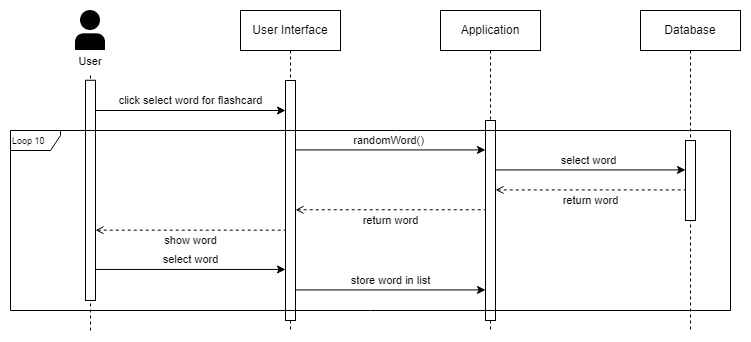
\includegraphics[width=\textwidth, keepaspectratio=true]{image/chap3/sequence/Flash-Select.jpg}
	\caption{แผนผังการทำงานแบบลำดับปฏิสัมพันธ์ของการเลือกคำศัพท์เพื่อใช้งานบัตรคำ}\label{fig:S_SelectFlashcard}
\end{figure}

\subsubsection{สุ่มคำศัพท์เพื่อใช้งานบัตรคำ}
\hspace{1cm}
เมื่อผู้ใช้กดปุ่มสุ่มคำศัพท์เพื่อใช้งานบัตรคำ UI จะสุ่มคำศัพท์และร้องข้อมูลคำศัพท์จากฐานข้อมูลผ่าน Application 
และฐานข้อมูลจะส่งข้อมูลกลับมาที่ Application และทำการเก็บข้อมูลไว้ จากนั้นจะทำการสุ่มคำศัพท์ใหม่จนครบ 10 คำ
\begin{figure}[!h]\centering
	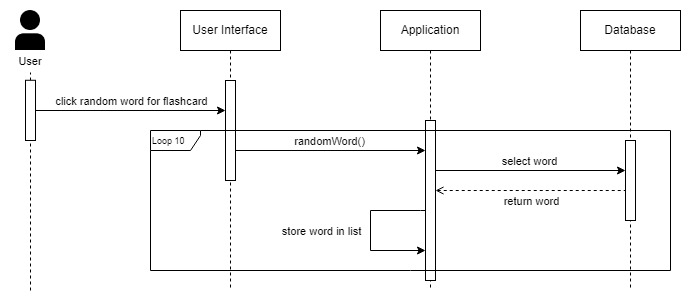
\includegraphics[width=\textwidth, keepaspectratio=true]{image/chap3/sequence/Flash-Random.jpg}
	\caption{แผนผังการทำงานแบบลำดับปฏิสัมพันธ์ของการสุ่มคำศัพท์เพื่อใช้งานบัตรคำ}\label{fig:S_RandomFlashcard}
\end{figure}

\pagebreak
\subsubsection{ดูบัตรคำ}
\hspace{1cm}
UI จะร้องขอข้อมูลคำศัพท์ที่เก็บไว้ใน Application มาทำการแสดงผลด้านหน้าของบัตรคำ และเมื่อผู้ใช้กดที่บัตรคำ UI จะทำการแสดงผลด้านหลังของบัตรคำ
และเมื่อผู้ใช้กดจำบัตรคำ UI จะทำการลบคำดังกล่าวและร้องขอข้อมูลคำศัพท์ถัดไปจาก Application และ Application จะทำการส่งข้อมูลคำศัพท์เข้าไปเก็บเป็นคำศัพท์ที่เรียนแล้ว
ในฐานข้อมูล แล้วจึงส่งข้อมูลคำศัพท์ถัดไปมาให้ UI เพื่อแสดงผล จากนั้นจะทำการแสดงผลคำศัพท์ถัดไปจนไม่เหลือคำศัพท์อยู่
\begin{figure}[!h]\centering
	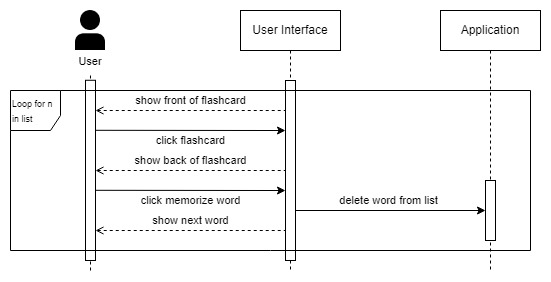
\includegraphics[width=\textwidth, keepaspectratio=true]{image/chap3/sequence/Flashcard.jpg}
	\caption{แผนผังการทำงานแบบลำดับปฏิสัมพันธ์ของการดูบัตรคำ}\label{fig:S_Flashcard}
\end{figure}

\pagebreak
\subsubsection{ทำแบบทดสอบ}
\hspace{1cm}
เมื่อผู้ใช้กดปุ่มเริ่มทำแบบทดสอบ ระบบจะทำการสุ่มคำศัพท์จำนวน 10 คำมาเก็บไว้ใน Application จากนั้นจะส่งรายการคำศัพท์ไปให้ UI เพื่อทำการแสดงแบบทดสอบ 
เมื่อ UI แสดงแบบทดสอบแล้ว ผู้ใช้จะตอบคำถาม จากนั้น UI จะแสดงผลคำตอบที่ถูกต้อง แล้ววนซ้ำการแสดงผลแบบทดสอบจนครบ 10 รอบ จากนั้นจึงแสดงผลลัพท์ของการทำแบบทดสอบ
\begin{figure}[!h]\centering
	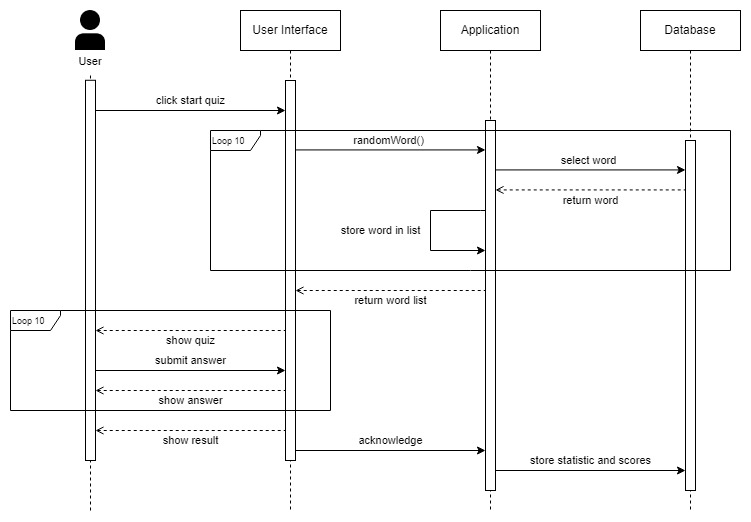
\includegraphics[width=\textwidth, keepaspectratio=true]{image/chap3/sequence/Quiz.jpg}
	\caption{แผนผังการทำงานแบบลำดับปฏิสัมพันธ์ของการทำแบบทดสอบ}\label{fig:S_Quiz}
\end{figure}

\pagebreak
\subsubsection{เล่นเกมเรียงพยัญชนะเป็นคำศัพท์}
\hspace{1cm}
เมื่อผู้ใช้กดปุ่มเริ่มเล่นเกมระบบจะทำการสุ่มคำศัพท์จากฐานข้อมูลผ่าน Application เพื่อทำการแสดงผลคำศัพท์ที่ใช้เล่นเกม เมื่อได้คำศัพท์แล้ว
UI จะแสดงผลคำศัพท์ที่ใช้เล่นเกม ผู้ใช้จะใส่คำตอบ จากนั้น UI จะแสดงผลคำตอบที่ถูกต้อง จากนั้นจึงแสดงผลลัพท์ของการเล่นเกม
\begin{figure}[!h]\centering
	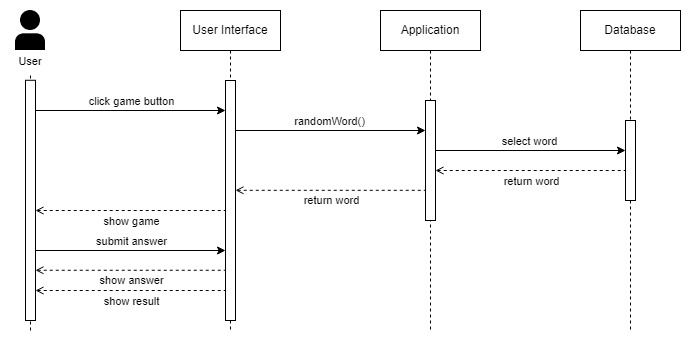
\includegraphics[width=\textwidth, keepaspectratio=true]{image/chap3/sequence/Game.jpg}
	\caption{แผนผังการทำงานแบบลำดับปฏิสัมพันธ์ของการเล่นเกมเรียงพยัญชนะเป็นคำศัพท์}\label{fig:S_Game}
\end{figure}

\pagebreak
\subsection{User Interface Design}
\begin{figure}[!h]\centering
	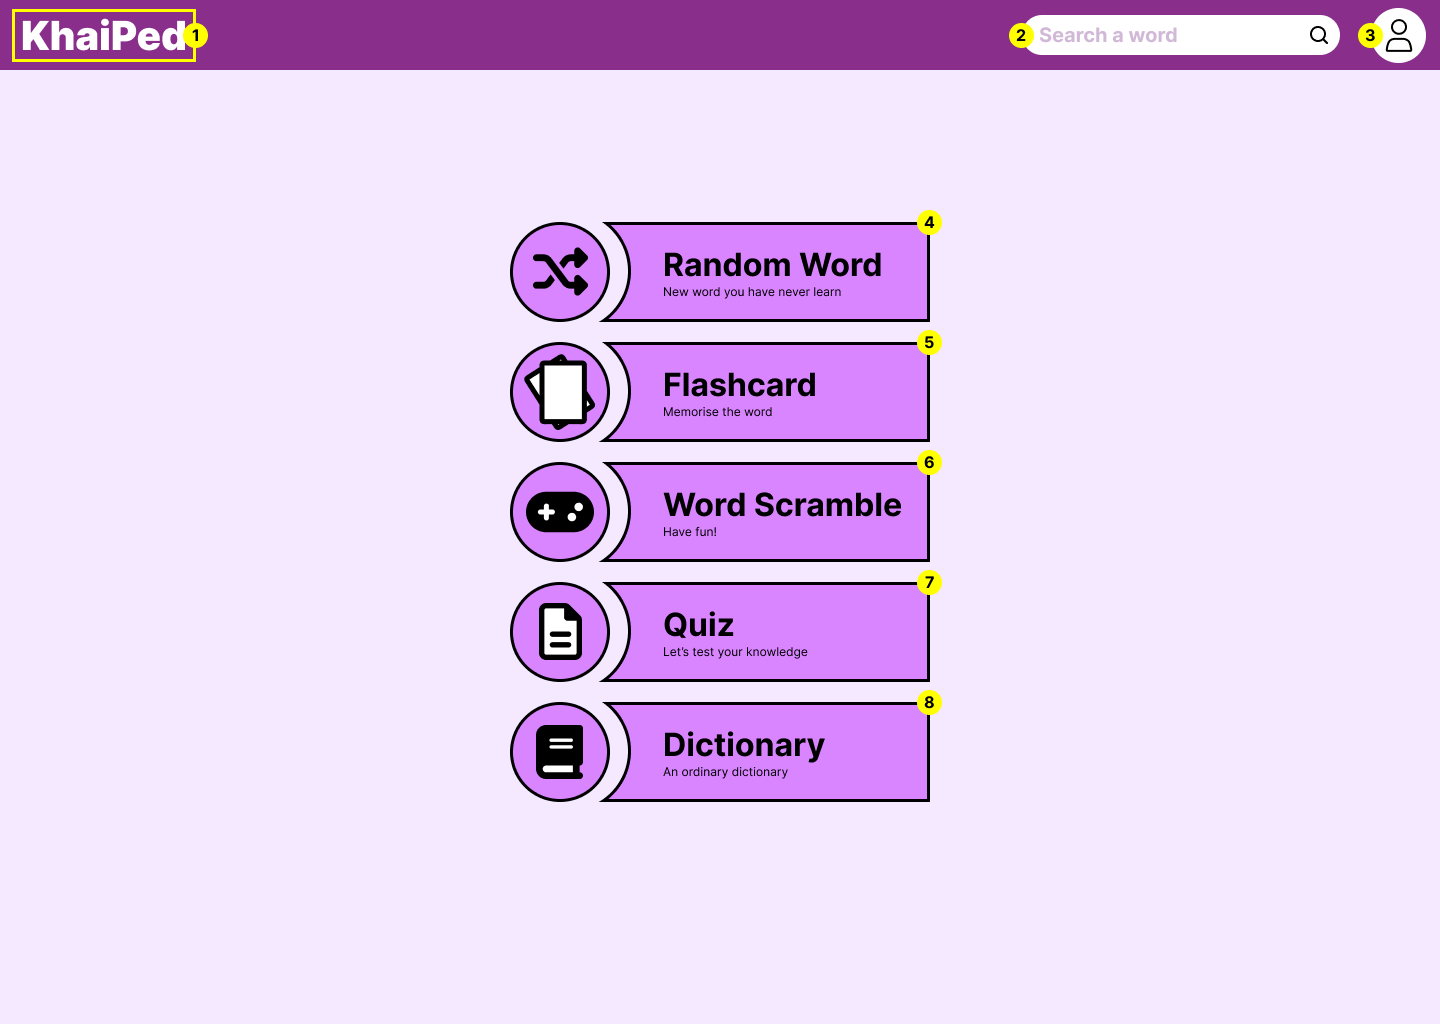
\includegraphics[width=\textwidth, keepaspectratio=true]{image/chap3/ui/Home page.png}
	\caption{หน้าหลัก}\label{fig:UI_Home}
\end{figure}
\hspace{1cm}
หน้าหลักสำหรับผู้ใช้งาน ประกอบด้วยปุ่มโลโก้ (1) ที่สามารถกดเพื่อกลับมาหน้าหลักได้ ช่องค้นหาคำศัพท์ (2) เพื่อค้นหาคำศัพท์ในฐานข้อมูล 
ปุ่มผู้ใช้ (3) สำหรับลงทะเบียนหรือเข้าสู่ระบบ และปุ่มสำหรับการใช้งานฟีเจอร์ต่าง ๆ ของระบบ ประกอบด้วย 
ปุ่มสุ่มคำศัพท์ (4) เพื่อสุ่มคำศัพท์ภาษาอังกฤษใหม่ ๆ ที่ยังไม่เคยเรียน ปุ่มบัตรคำ (5) เพื่อใช้งานบัตรคำ ปุ่มเล่นเกม (6) เพื่อเล่นเกมเรียงพยัญชนะเป็นคำศัพท์ 
ปุ่มทำแบบทดสอบ (7) เพื่อเข้าทำแบบทดสอบ และปุ่มพจนานุกรม (8) เพื่อใช้งานพจนานุกรม

\pagebreak
\begin{figure}[!h]\centering
	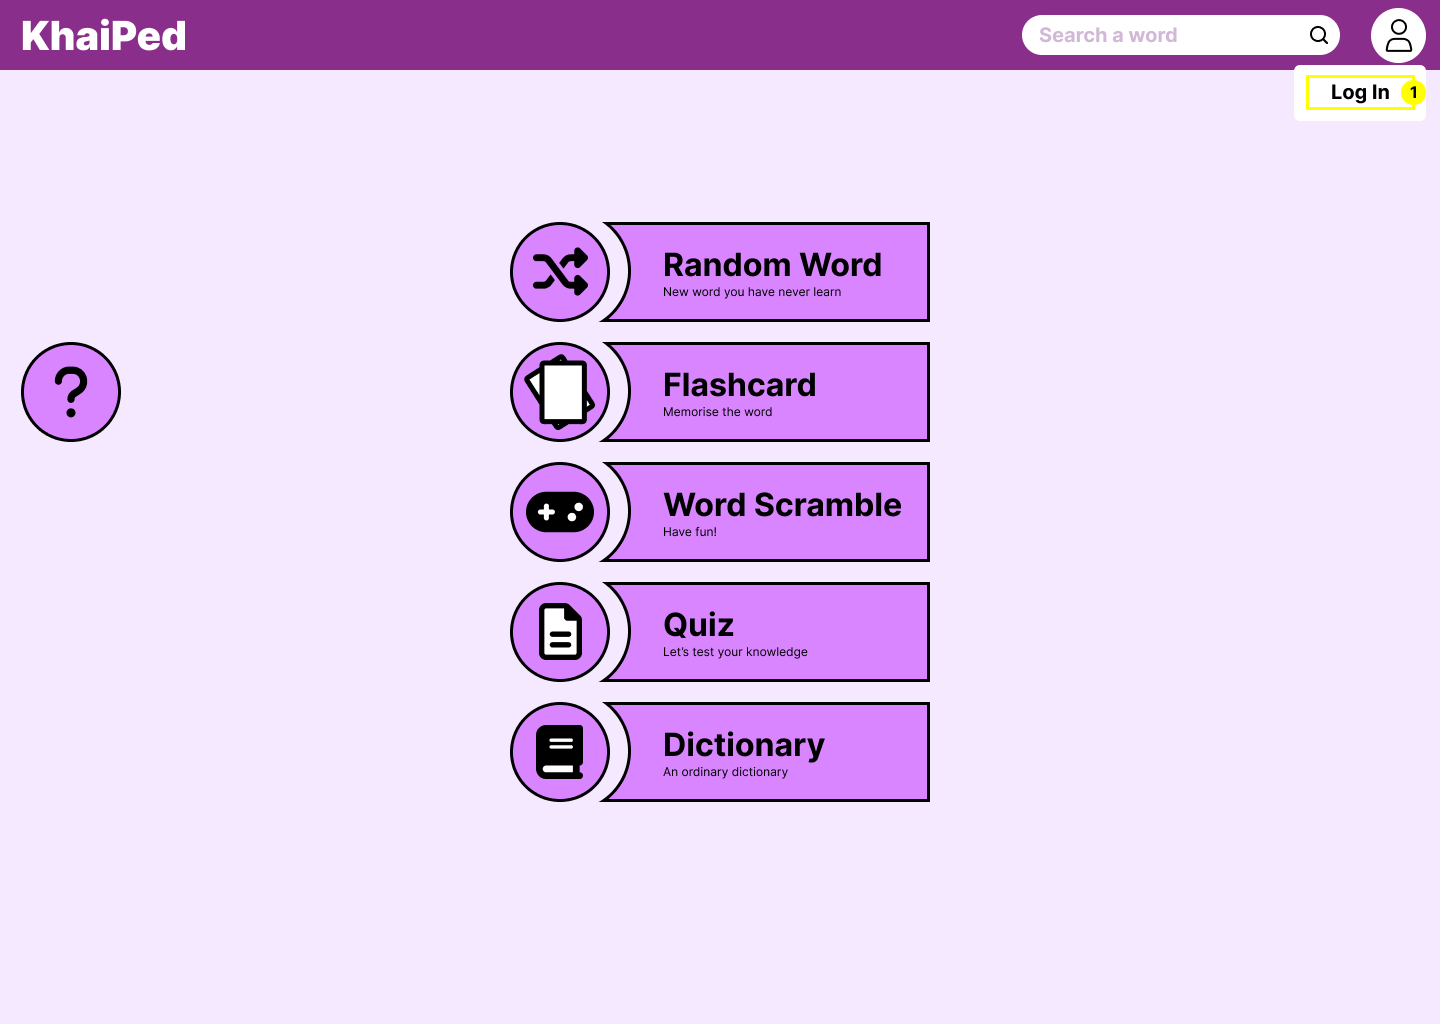
\includegraphics[width=0.8\textwidth, keepaspectratio=true]{image/chap3/ui/login/Home page - Guest User Button.png}
	\caption{ปุ่มผู้ใช้หากไม่ได้เข้าสู่ระบบ}\label{fig:UI_GuestButton}
\end{figure}
\hspace{1cm}
เมื่อผู้ใช้งานกดปุ่มผู้ใช้โดยที่ยังไม่ได้เข้าสู่ระบบ จะระบบจะแสดงปุ่มเข้าสู่ระบบ (1) สำหรับผู้ใช้งานที่มีบัญชีอยู่แล้วเพื่อเข้าสู่ระบบ

\begin{figure}[!h]\centering
	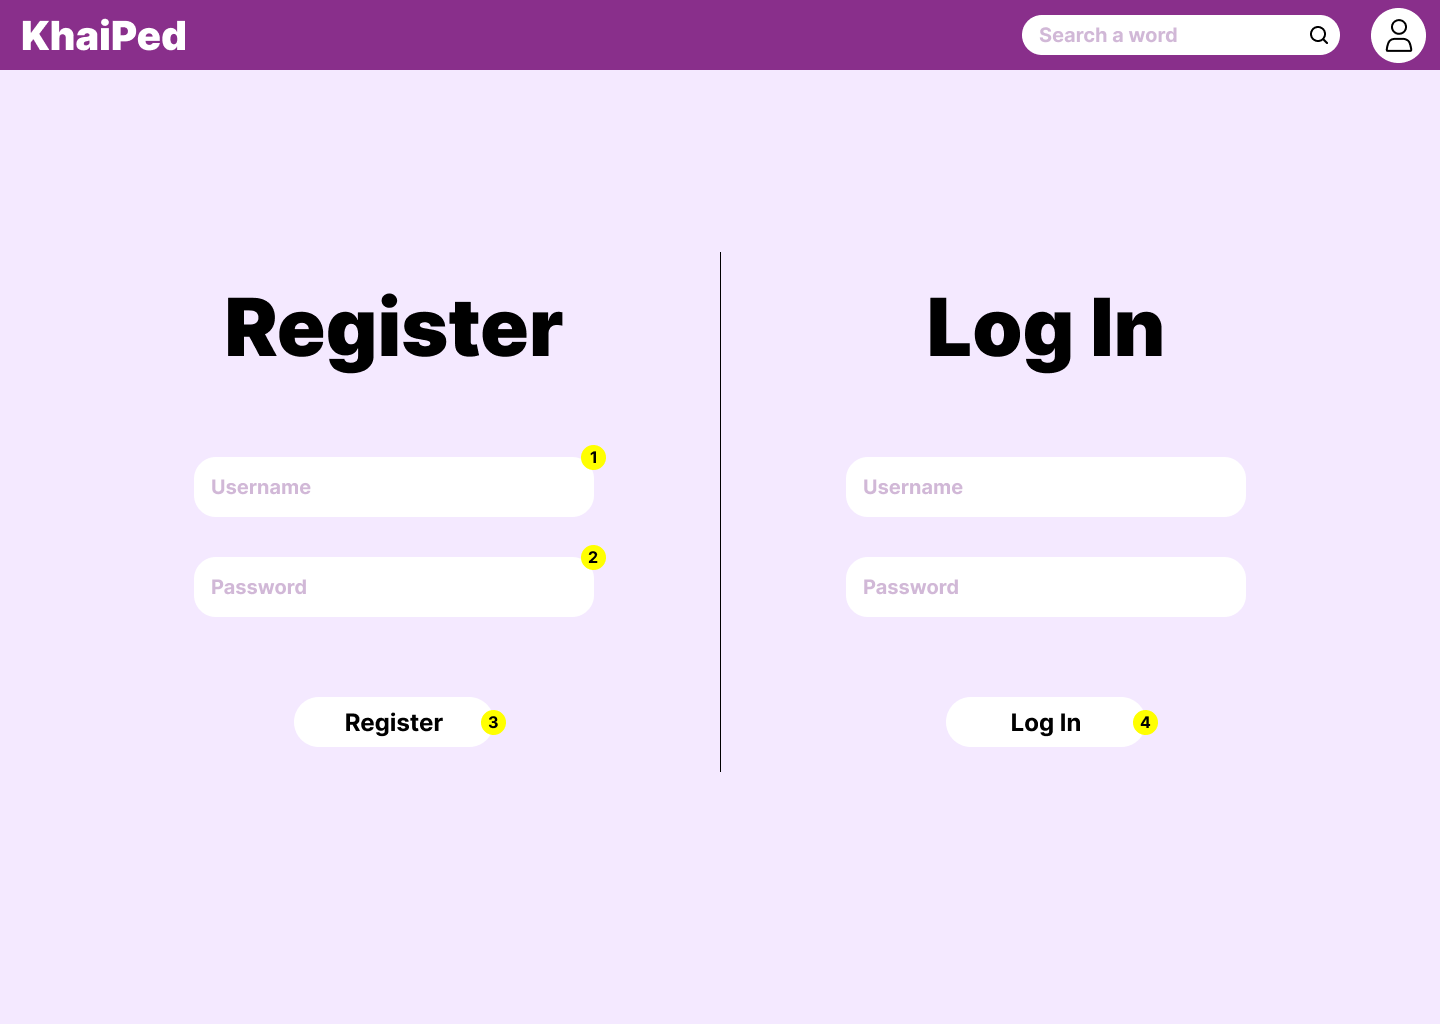
\includegraphics[width=0.8\textwidth, keepaspectratio=true]{image/chap3/ui/login/Home page - Register.png}
	\caption{หน้าลงทะเบียนและเข้าสู่ระบบ}\label{fig:UI_LoginPage}
\end{figure}
\hspace{1cm}
เมื่อผู้ใช้งานกดปุ่มลงทะเบียน ระบบจะแสดงผลหน้าลงทะเบียนและเข้าสู่ระบบ โดยจะประกอบไปด้วยส่วนสำหรับใส่ชื่อผู้ใช้งาน (1) 
ส่วนสำหรับใส่รหัสผ่าน (2) ปุ่มลงทะเบียน (3) และ ปุ่มเข้าสู่ระบบ (4)

\pagebreak
\begin{figure}[!h]\centering
	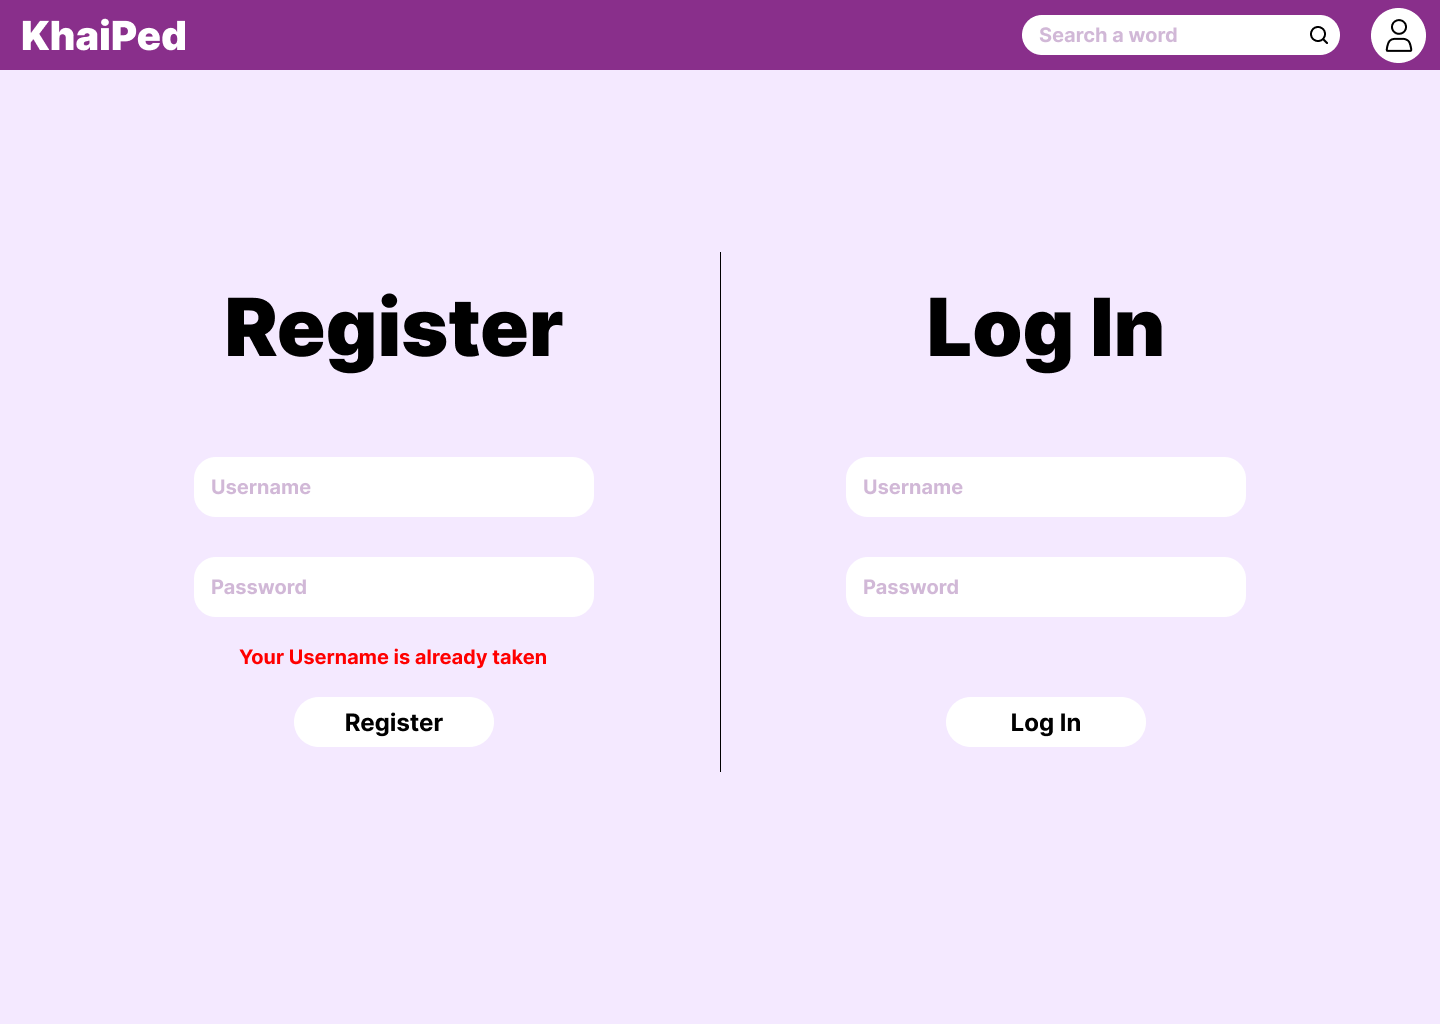
\includegraphics[width=0.8\textwidth, keepaspectratio=true]{image/chap3/ui/login/Home page - Register error.png}
	\caption{ข้อผิดพลาดในการลงทะเบียน}\label{fig:UI_RegisterError}
\end{figure}
\hspace{1cm}
หากผู้ใช้งานกรอกชื่อผู้ใช้งานที่ซ้ำกับในระบบ ระบบจะแจ้งเตือนว่าชื่อผู้ใช้งานได้ถูกใช้ไปแล้ว

\begin{figure}[!h]\centering
	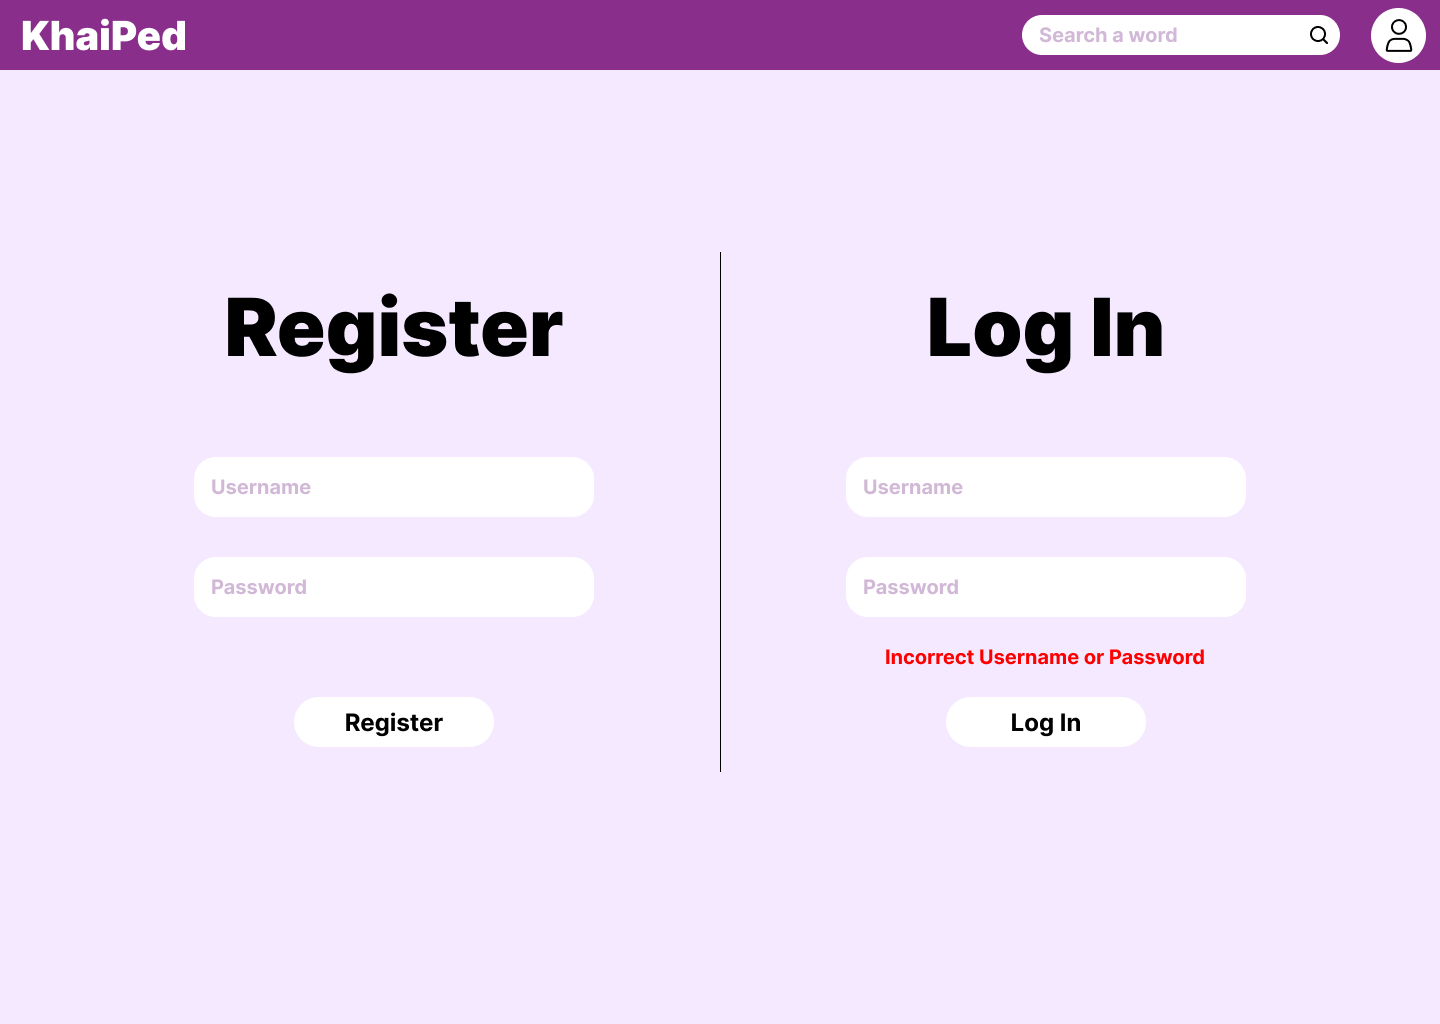
\includegraphics[width=0.8\textwidth, keepaspectratio=true]{image/chap3/ui/login/Home page - Log in error.png}
	\caption{ข้อผิดพลาดในการเข้าสู่ระบบ}\label{fig:UI_LogInError}
\end{figure}
\hspace{1cm}
หากผู้ใช้งานกรอกชื่อผู้ใช้งานหรือรหัสผ่านผิด ระบบจะแจ้งเตือนว่าชื่อผู้ใช้งานหรือรหัสผ่านผิด

\pagebreak
\begin{figure}[!h]\centering
	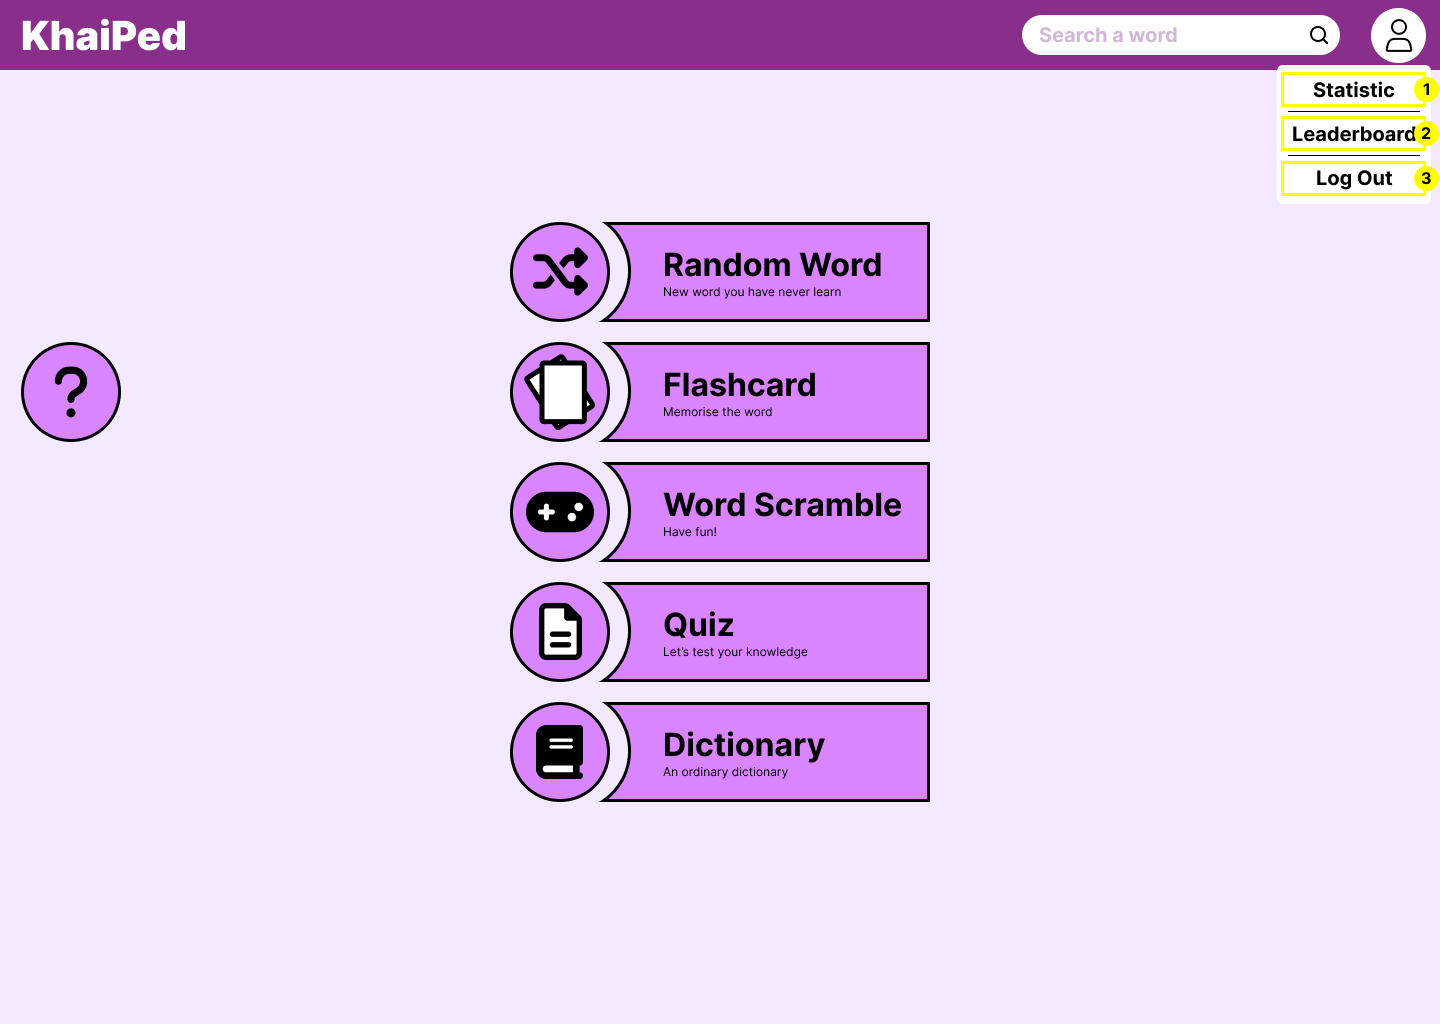
\includegraphics[width=0.8\textwidth, keepaspectratio=true]{image/chap3/ui/statistic/Home page - Logged In User Button.png}
	\caption{ปุ่มผู้ใช้หากเข้าสู่ระบบแล้ว}\label{fig:UI_UserButton}
\end{figure}
\hspace{1cm}
เมื่อผู้ใช้งานกดปุ่มผู้ใช้โดยที่เข้าสู่ระบบแล้ว จะระบบจะแสดงปุ่มสองปุ่มคือ ปุ่มสถิติ (1) เพื่อเข้าสู่หน้าแสดงผลสถิติการใช้เว็บแอปพลิเคชันของผู้ใช้ และปุ่มลงชื่อออก (2) 

\begin{figure}[!h]\centering
	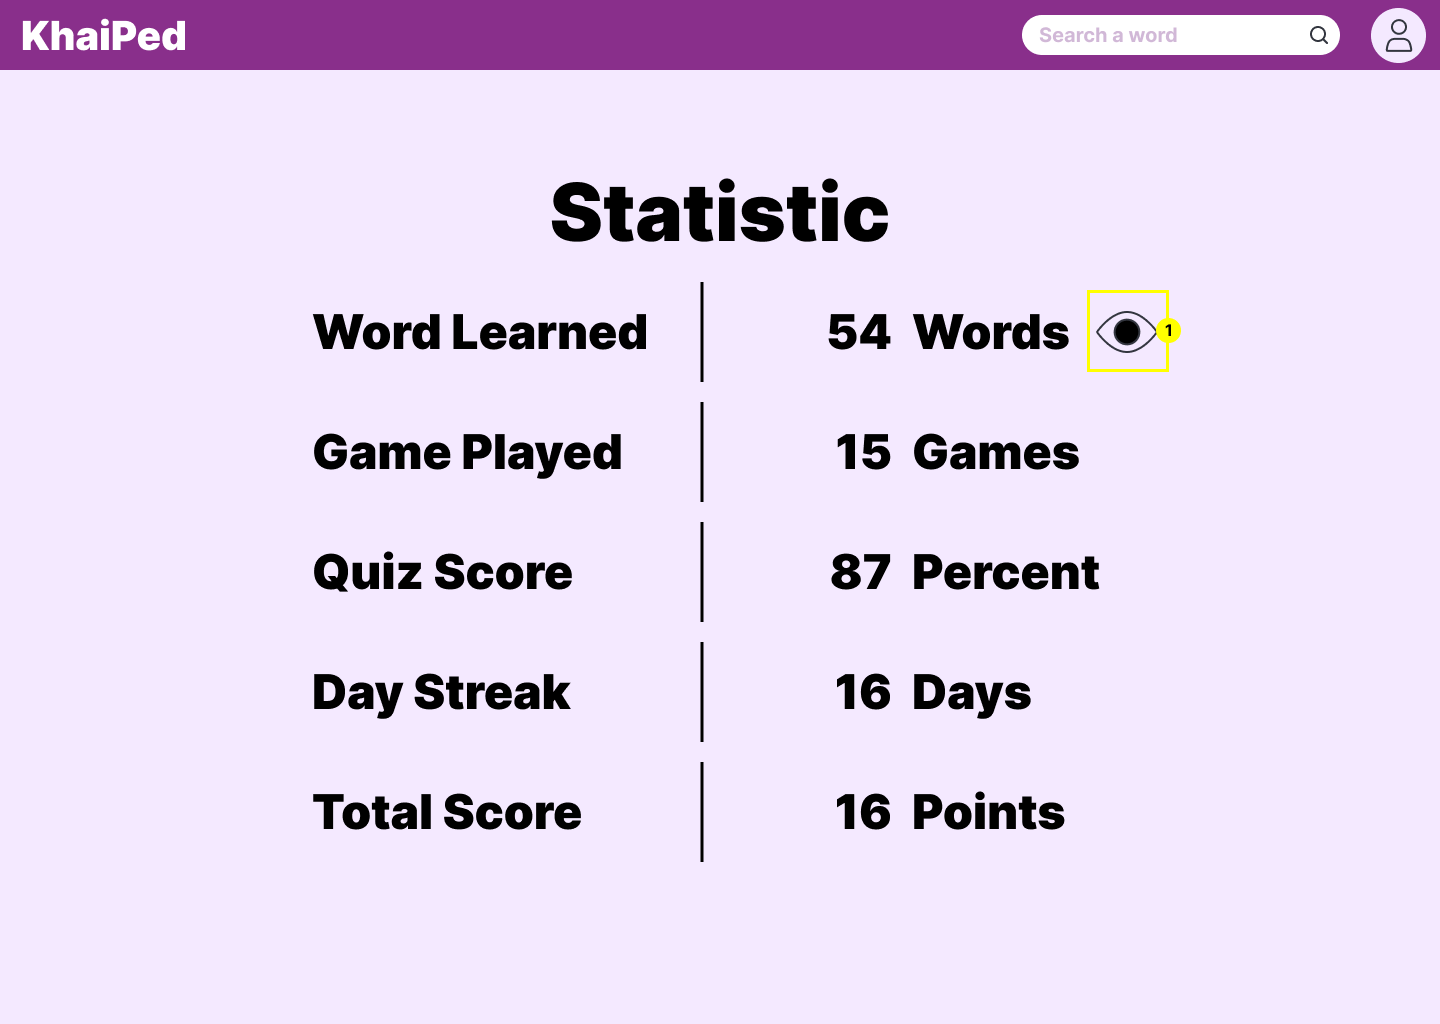
\includegraphics[width=0.8\textwidth, keepaspectratio=true]{image/chap3/ui/statistic/Statistic.png}
	\caption{หน้าสถิติการใช้งานเว็บแอปพลิเคชัน}\label{fig:UI_Statistic}
\end{figure}
\hspace{1cm}
เมื่อผู้ใช้งานกดปุ่มสถิติ ระบบจะแสดงผลหน้าสถิติซึ่งประกอบไปด้วยจำนวนคำที่เคยเรียน จำนวนเกมที่ได้เล่นไป คะแนนของแบบทดสอบโดยคิดเป็นเปอร์เซ็นต์ และจำนวนวันที่เข้าใช้งานติดต่อกัน

\pagebreak
\begin{figure}[!h]\centering
	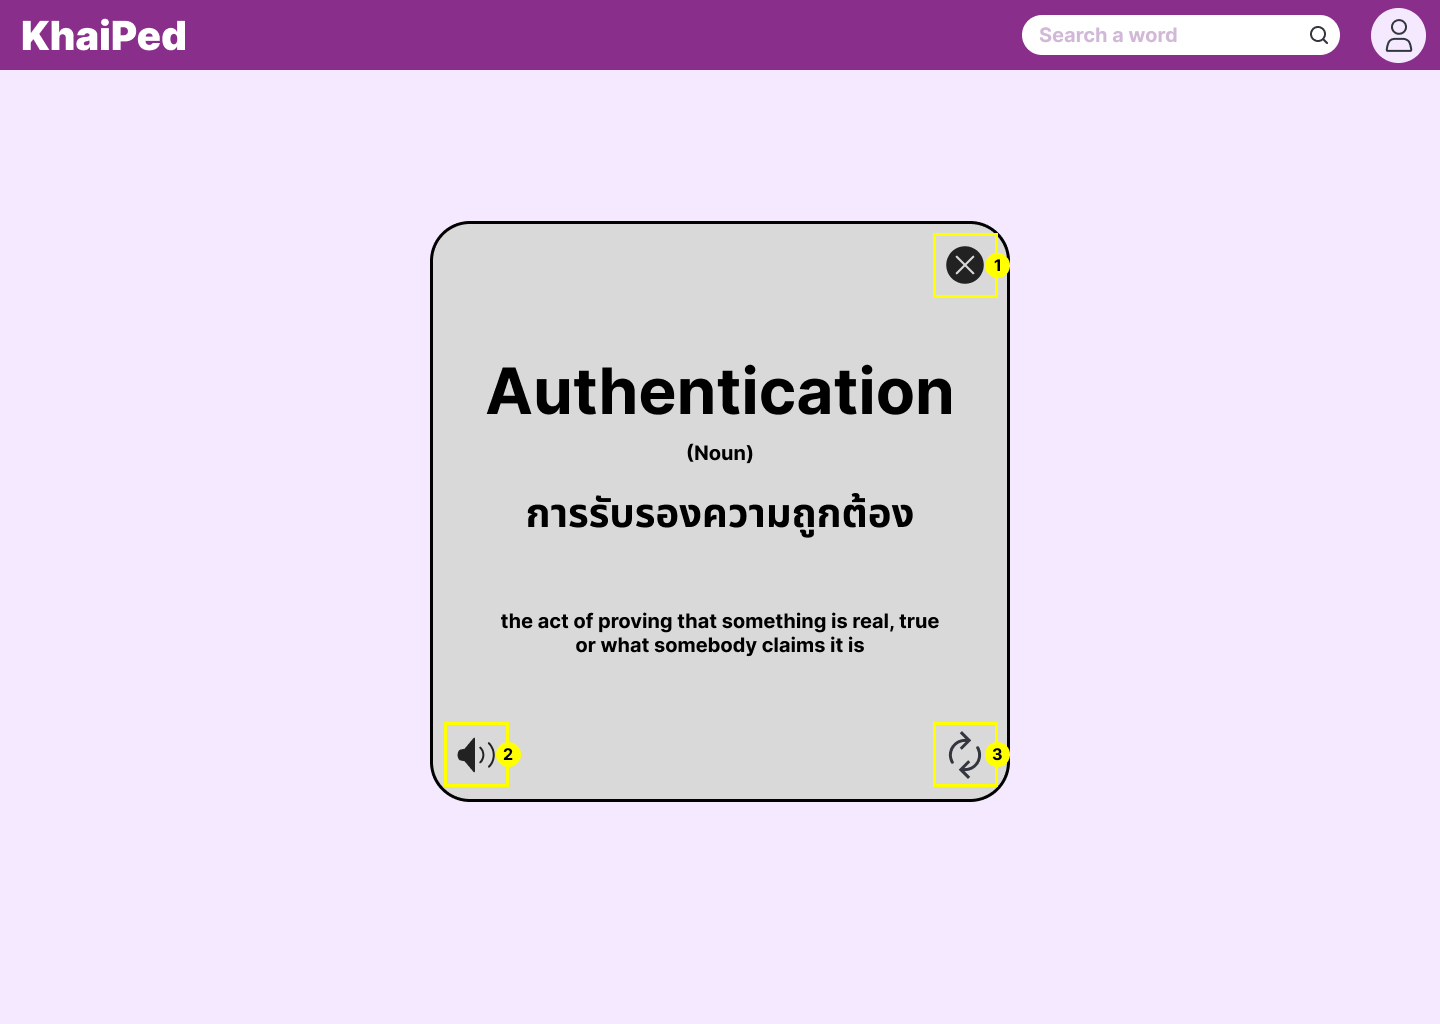
\includegraphics[width=0.8\textwidth, keepaspectratio=true]{image/chap3/ui/Random Word.png}
	\caption{การสุ่มคำศัพท์ใหม่เพื่อการเรียนรู้}\label{fig:UI_RandomWord}
\end{figure}
\hspace{1cm}
เมื่อผู้ใช้กดปุ่มสุ่มคำศัพท์ในหน้าหลัก ระบบจะแสดงการ์ดคำศัพท์ที่สุ่มมา โดยในการ์ดจะประกอบไปด้วย คำศัพท์, Part of Speech, ความหมายภาษาไทยและอังกฤษ และปุ่มสามปุ่ม ได้แก่ปุ่มปิด (1) 
เมื่อกดแล้วจะกลับไปหน้าหลัก, ปุ่มเล่นเสียง (2) เมื่อกดแล้วระบบจะเล่นเสียงวิธีการออกเสียงของคำศัพท์ และปุ่มสุ่มคำใหม่ (3) เมื่อกดแล้วระบบจะสุ่มคำศัพท์ใหม่เพื่อแสดงผล

\begin{figure}[!h]\centering
	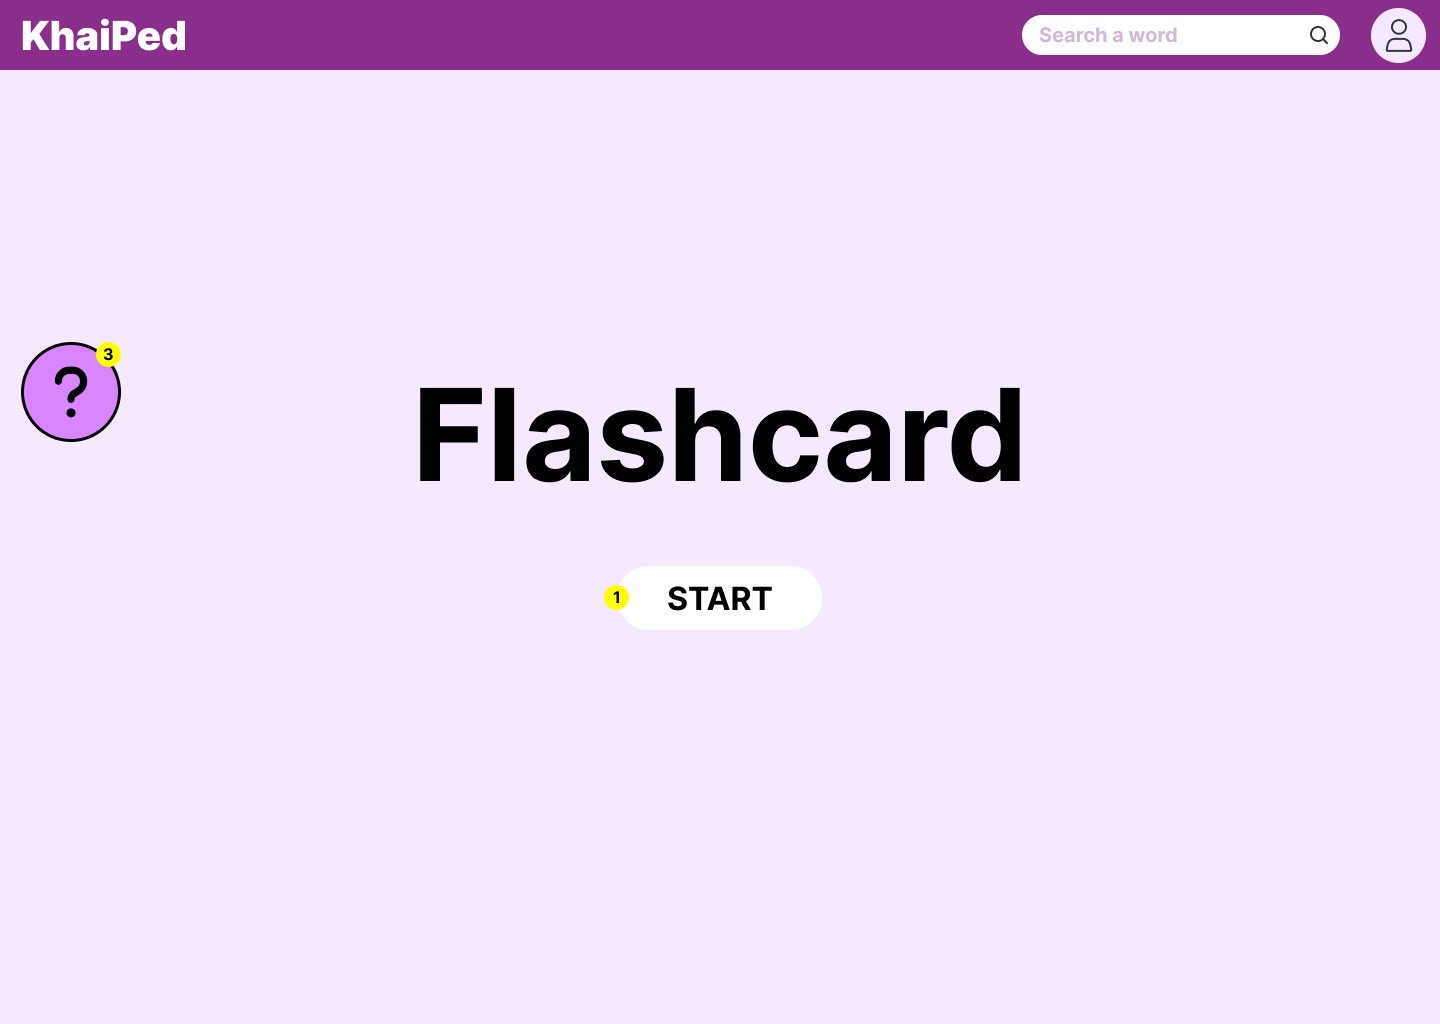
\includegraphics[width=0.8\textwidth, keepaspectratio=true]{image/chap3/ui/flashcard/Flashcard.png}
	\caption{หน้าหลักบัตรคำ}\label{fig:UI_Flashcard}
\end{figure}
\hspace{1cm}
เมื่อผู้ใช้กดปุ่มบัตรคำ ระบบจะแสดงผลหน้าบัตรคำ โดยในหน้าจะประกอบไปด้วยปุ่มสองปุ่ม ได้แก่ ปุ่มสุ่มคำศัพท์ (1) เมื่อกดแล้ว ระบบจะคำศัพท์จำนวน 10 คำ 
แล้วทำการแสดงผลบัตรคำ และปุ่มเลือกคำศัพท์ (2) โดยเมื่อกดแล้ว ระบบจะแสดงผลหน้าเลือกคำศัพท์เพื่อใช้กับบัตรคำ

\pagebreak
\begin{figure}[!h]\centering
	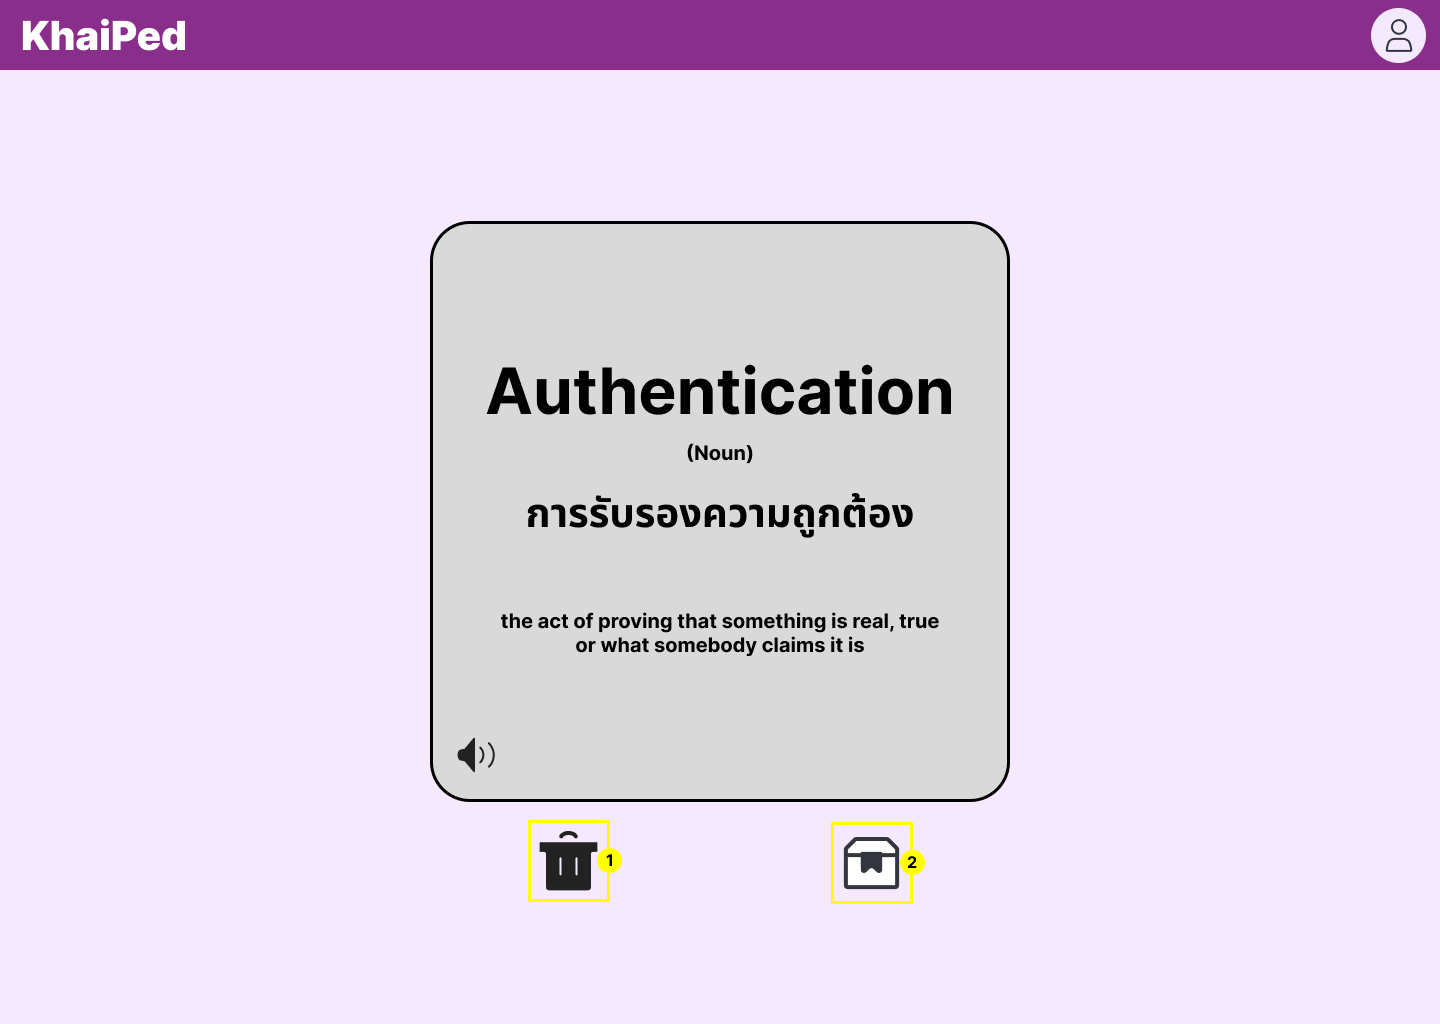
\includegraphics[width=0.8\textwidth, keepaspectratio=true]{image/chap3/ui/flashcard/Flashcard - Select Word.png}
	\caption{หน้าเลือกคำศัพท์เพื่อใช้งานบัตรคำ}\label{fig:UI_SelectFlashcard1}
\end{figure}
\hspace{1cm}
เมื่อผู้ใช้กดปุ่มเลือกคำศัพท์ ระบบจะแสดงการ์ดคำศัพท์ ซึ่งจะมีรายละเอียดของคำศัพท์อยู่บนการ์ด โดยจะมีปุ่มเล่นเสียง ปุ่มทิ้งคำศัพท์ (1)
เมื่อกดแล้วระบบจะสุ่มคำศัพท์ใหม่มาแสดงผลให้ผู้ใช้เลือก และปุ่มเก็บคำศัพท์ (2) เมื่อกดแล้วระบบจะเก็บคำศัพท์ที่เลือกแล้วแสดงผลคำศัพท์ใหม่

\begin{figure}[!h]\centering
	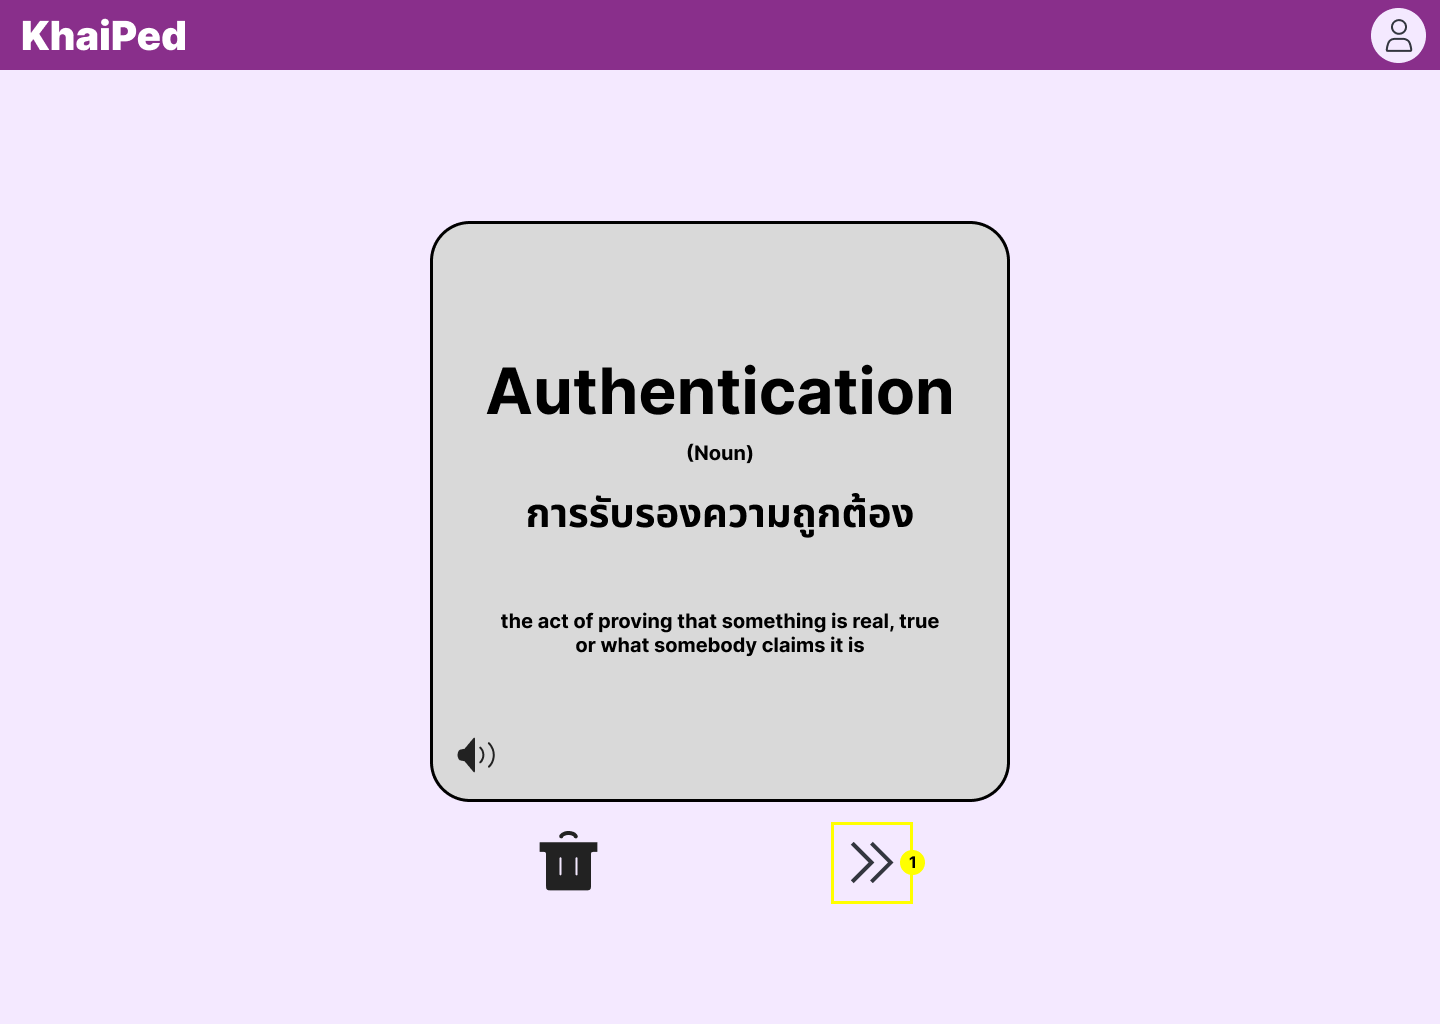
\includegraphics[width=0.8\textwidth, keepaspectratio=true]{image/chap3/ui/flashcard/Flashcard - Select Word-1.png}
	\caption{เมื่อเลือกคำศัพท์เพื่อใช้งานบัตรคำครบแล้ว}\label{fig:UI_SelectFlashcard2}
\end{figure}
\hspace{1cm}
เมื่อผู้ใช้กดปุ่มเก็บคำศัพท์จนระบบเก็บคำศัพท์ครบ 10 คำแล้ว ปุ่มเก็บคำศัพท์จะเปลี่ยนเป็นปุ่มถัดไป (1) เมื่อกดแล้วระบบจะแสดงผลบัตรคำที่เก็บไว้

\pagebreak
\begin{figure}[!h]\centering
	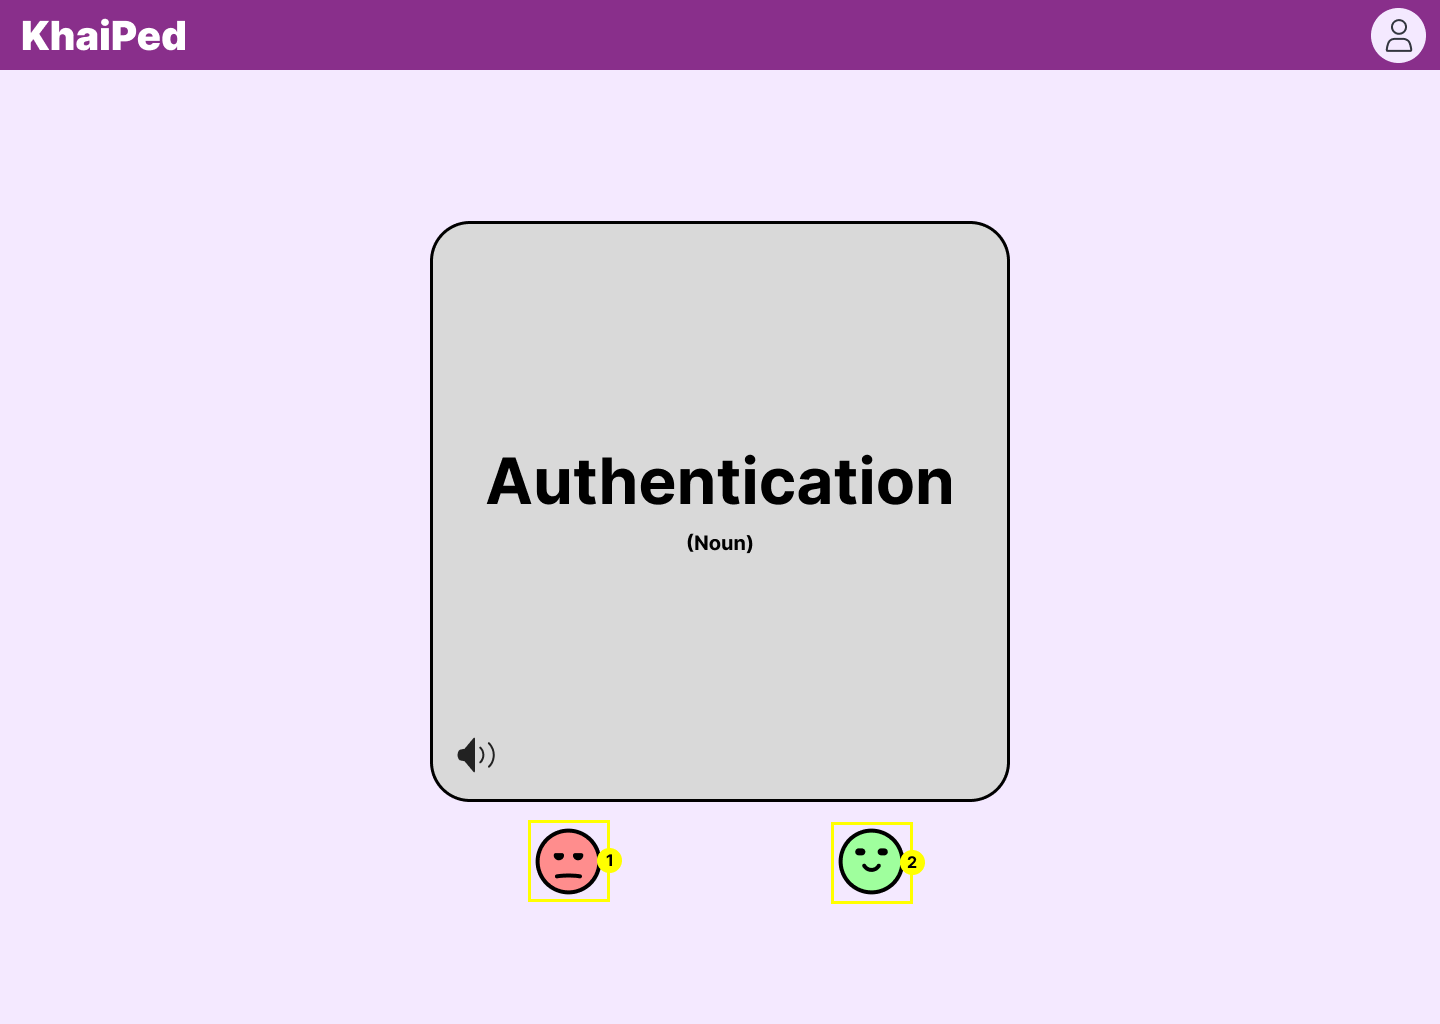
\includegraphics[width=0.8\textwidth, keepaspectratio=true]{image/chap3/ui/flashcard/Flashcard - Show Card.png}
	\caption{หน้าแสดงผลด้านหน้าบัตรคำ}\label{fig:UI_ShowCard}
\end{figure}
\hspace{1cm}
เมื่อผู้ใช้กดปุ่มสุ่มคำหรือเลือกคำครบ 10 คำแล้ว ระบบจะแสดงผลบัตรคำ โดยด้านหน้าของบัตรคำจะมีเพียงคำศัพท์ และ Part of Speech เมื่อผู้ใช้กดที่บัตรคำ
ระบบจะแสดงผลด้านหลังของบัตรคำ และผู้ใช้ยังสามารถกดปุ่มจำคำศัพท์ไม่ได้ (1) เมื่อกดแล้วระบบจะเก็บคำศัพท์นี้ไว้ และแสดงผลคำศัพท์ถัดไป และปุ่มจำศัพท์ได้ (2)
เมื่อกดแล้วระบบจะเก็บคำศัพท์นี้ไว้ และแสดงผลคำศัพท์ถัดไป

\begin{figure}[!h]\centering
	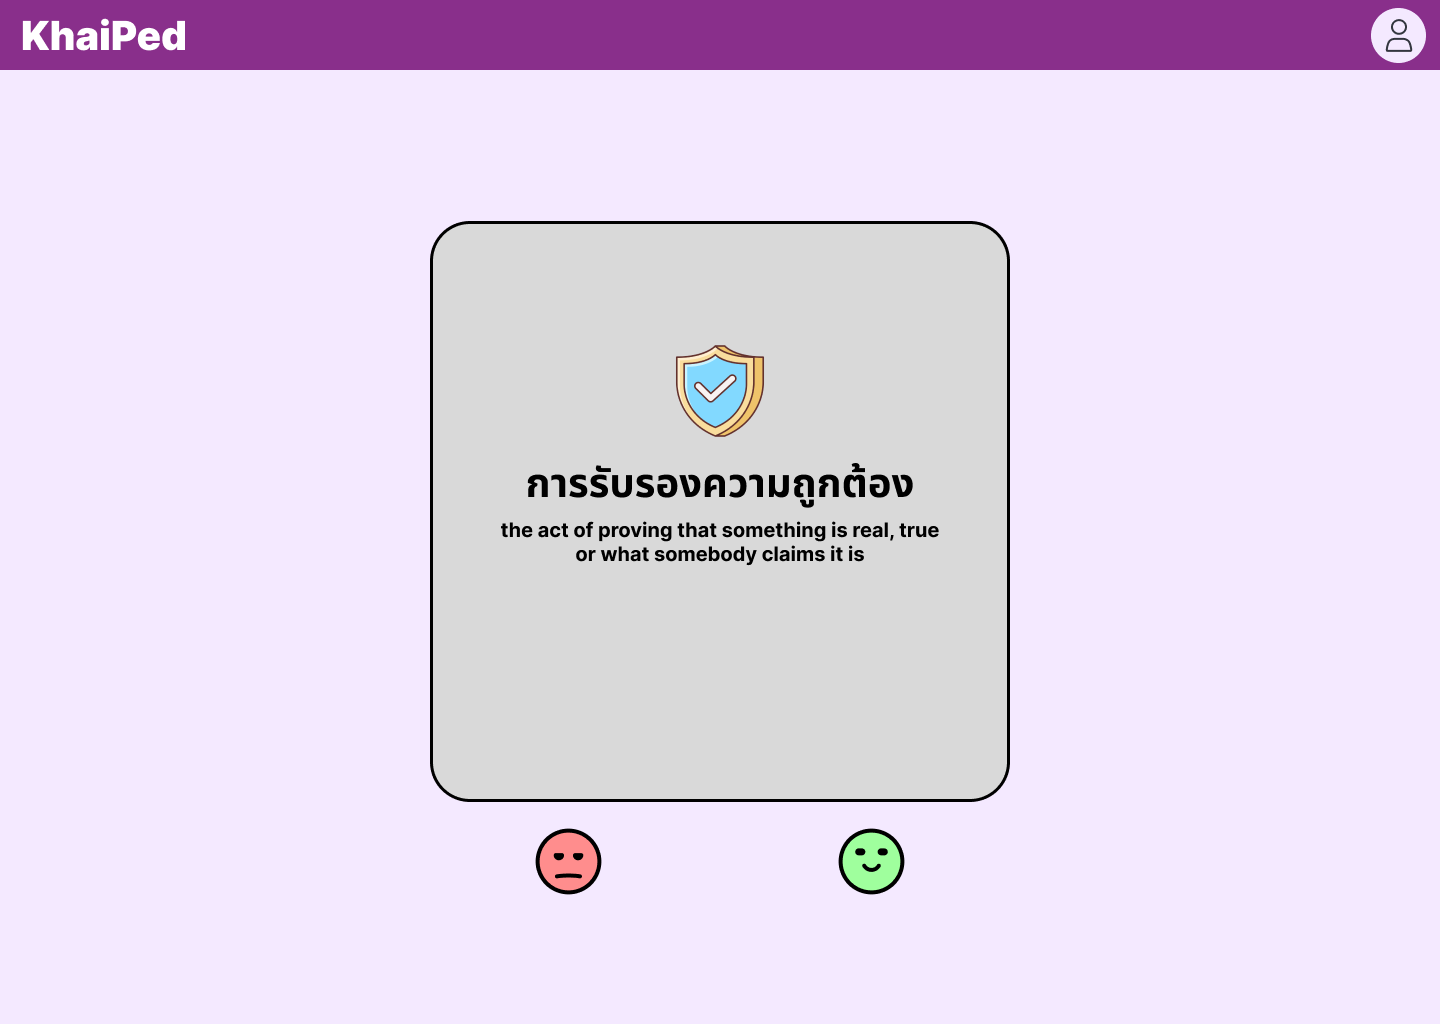
\includegraphics[width=0.8\textwidth, keepaspectratio=true]{image/chap3/ui/flashcard/Flashcard - Flip Card.png}
	\caption{หน้าแสดงผลด้านหลังบัตรคำ}\label{fig:UI_FlipCard}
\end{figure}
\hspace{1cm}
เมื่อผู้ใช้กดบัตรคำด้านหน้า ระบบจะแสดงผลบัตรคำด้านหลัง ซึ่งประกอบไปด้วยรูปภาพ และความหมายทั้งภาษาไทยและภาษาอังกฤษ

\pagebreak
\begin{figure}[!h]\centering
	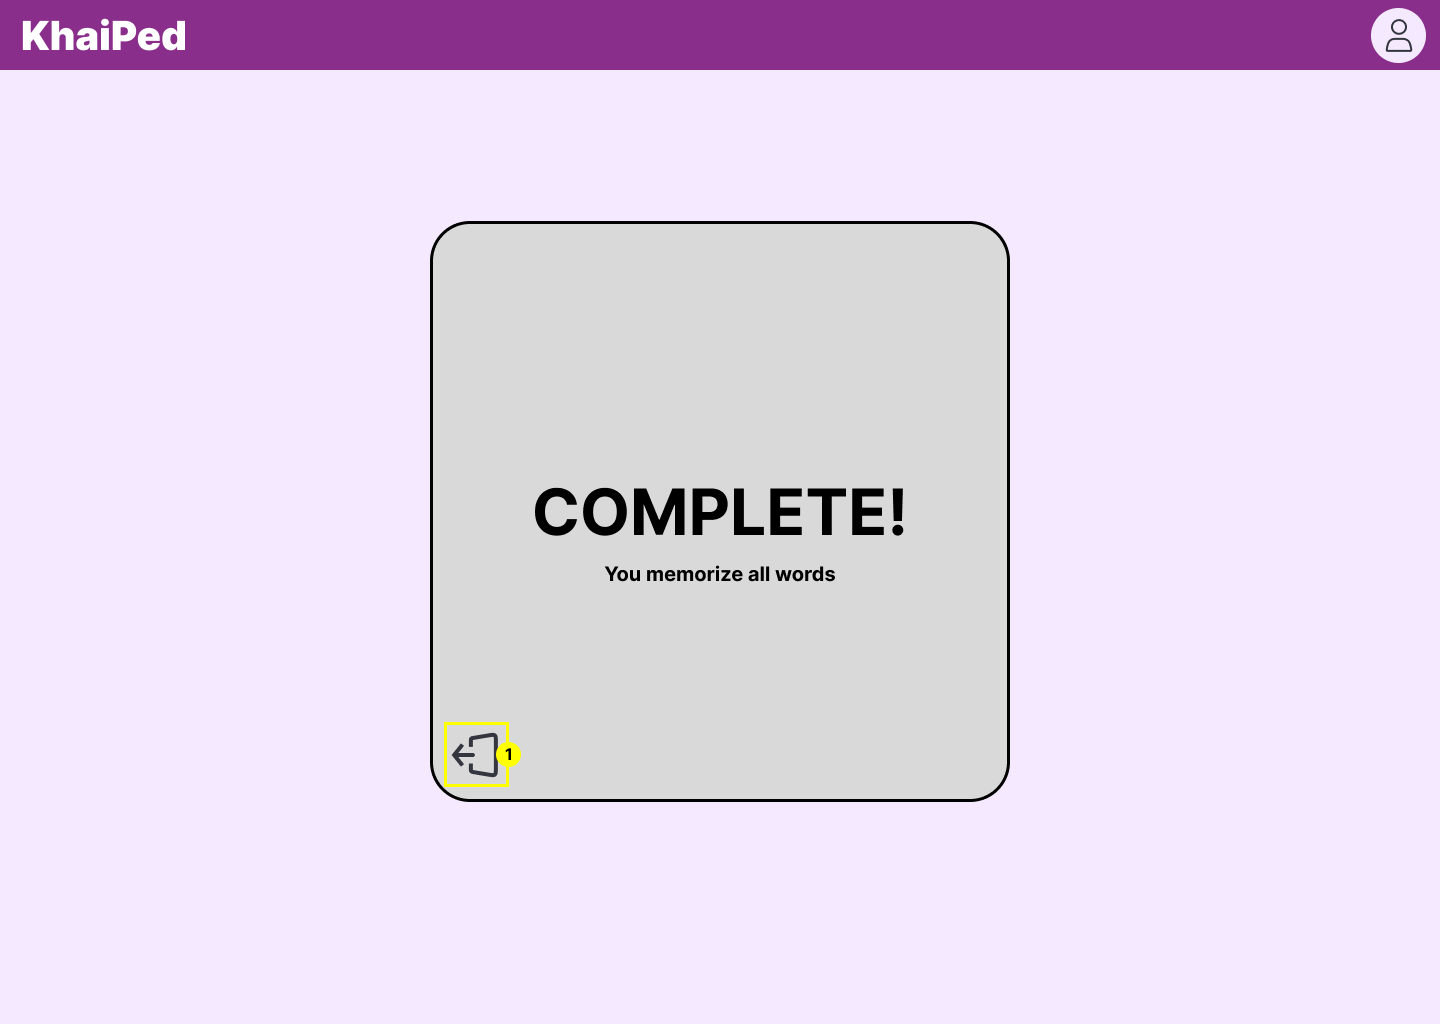
\includegraphics[width=0.8\textwidth, keepaspectratio=true]{image/chap3/ui/flashcard/Flashcard - Complete.png}
	\caption{หน้าแสดงผลการใช้บัตรคำ}\label{fig:UI_SelectFlashcard1}
\end{figure}
\hspace{1cm}
เมื่อผู้ใช้กดปุ่มจำศัพท์ได้จนไม่เหลือคำศัพท์แล้ว ระบบจะแสดงผลว่าผู้ใช้จำศัพท์ได้ครบแล้ว และสามารถกดปุ่มออก (1) เพื่อกลับไปหน้าหลักได้

\begin{figure}[!h]\centering
	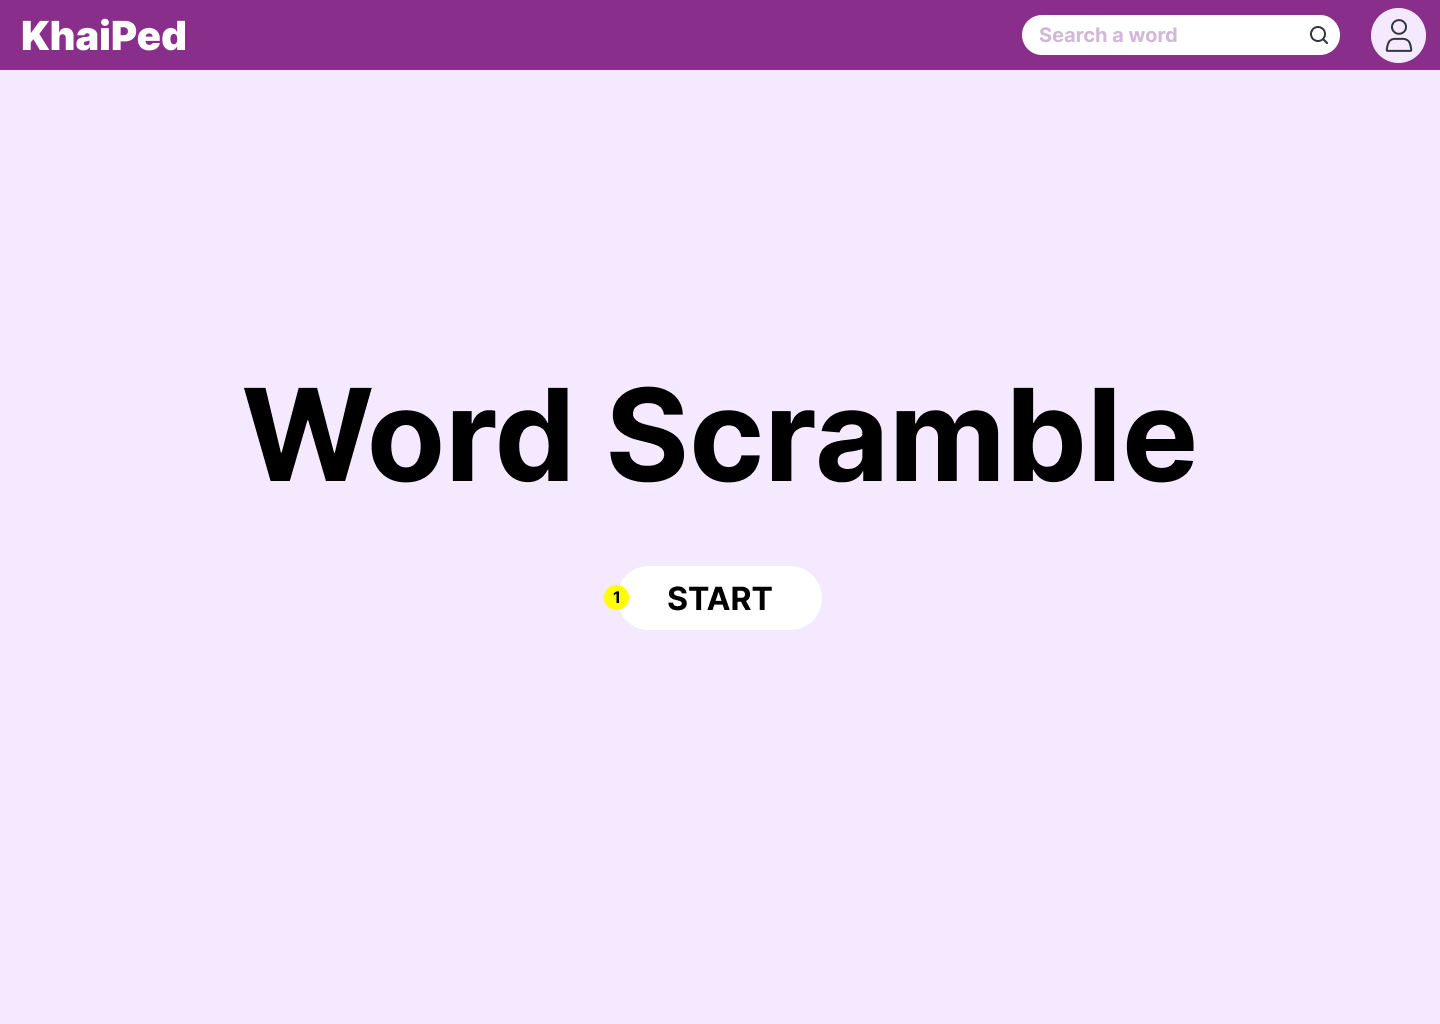
\includegraphics[width=0.8\textwidth, keepaspectratio=true]{image/chap3/ui/game/Word Scramble.png}
	\caption{หน้าหลักการเล่นเกมเรียงพยัญชนะเป็นคำศัพท์}\label{fig:UI_Game}
\end{figure}
\hspace{1cm}
เมื่อผู้ใช้กดปุ่มเล่นเกมในหน้าหลัก ระบบจะแสดงผลหน้าเล่นเกมโดยในหน้าจะประกอบไปด้วย
ปุ่มเริ่มเล่นเกม (1) เมื่อกดแล้ว ระบบจะทำการสุ่มคำศัพท์และแสดงผลหน้าสำหรับเล่นเกม

\pagebreak
\begin{figure}[!h]\centering
	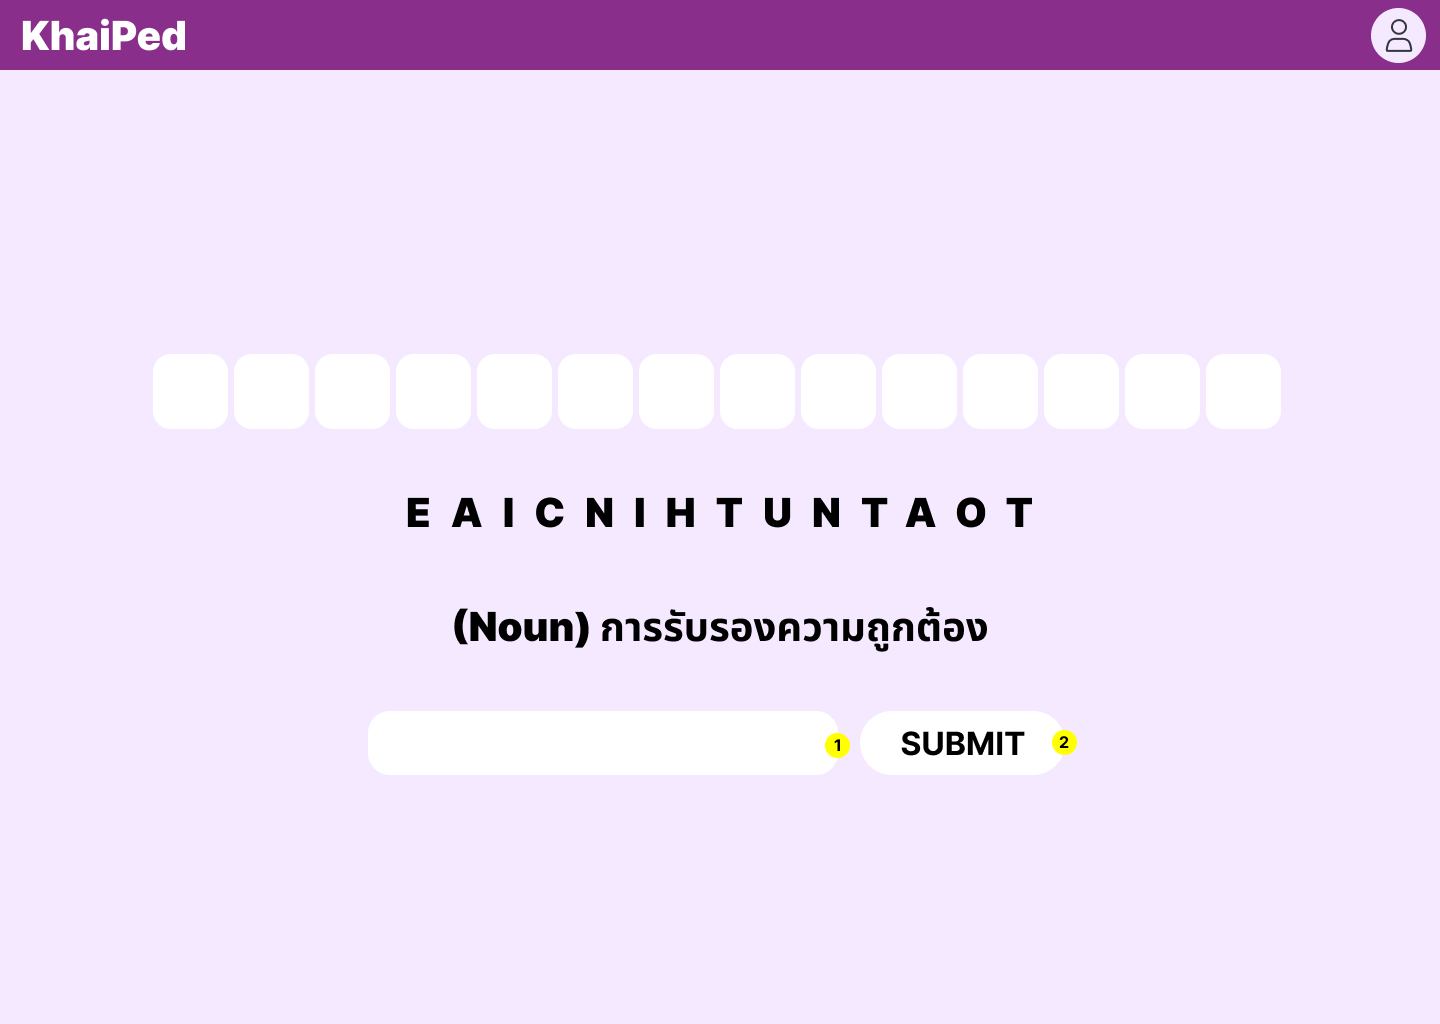
\includegraphics[width=0.8\textwidth, keepaspectratio=true]{image/chap3/ui/game/Word Scramble - Start.png}
	\caption{หน้าเล่นเกมเรียงพยัญชนะเป็นคำศัพท์}\label{fig:UI_StartGame}
\end{figure}
\hspace{1cm}
เมื่อผู้ใช้กดปุ่มปุ่มเริ่มเล่นเกม ระบบจะแสดงผลหน้าเล่นเกม โดยจะประกอบไปด้วยกล่องตัวอักษร สำหรับใส่ตัวอักษร ตัวอักษรที่ถูกสลับที่
และความหมายของคำ และปุ่มส่งคำศัพท์ (1) เมื่อกดแล้วระบบจะตรวจสอบว่าตัวอักษรที่ผู้ใช้ใส่ถูกตำแหน่งหรือไม่ 

\begin{figure}[!h]\centering
	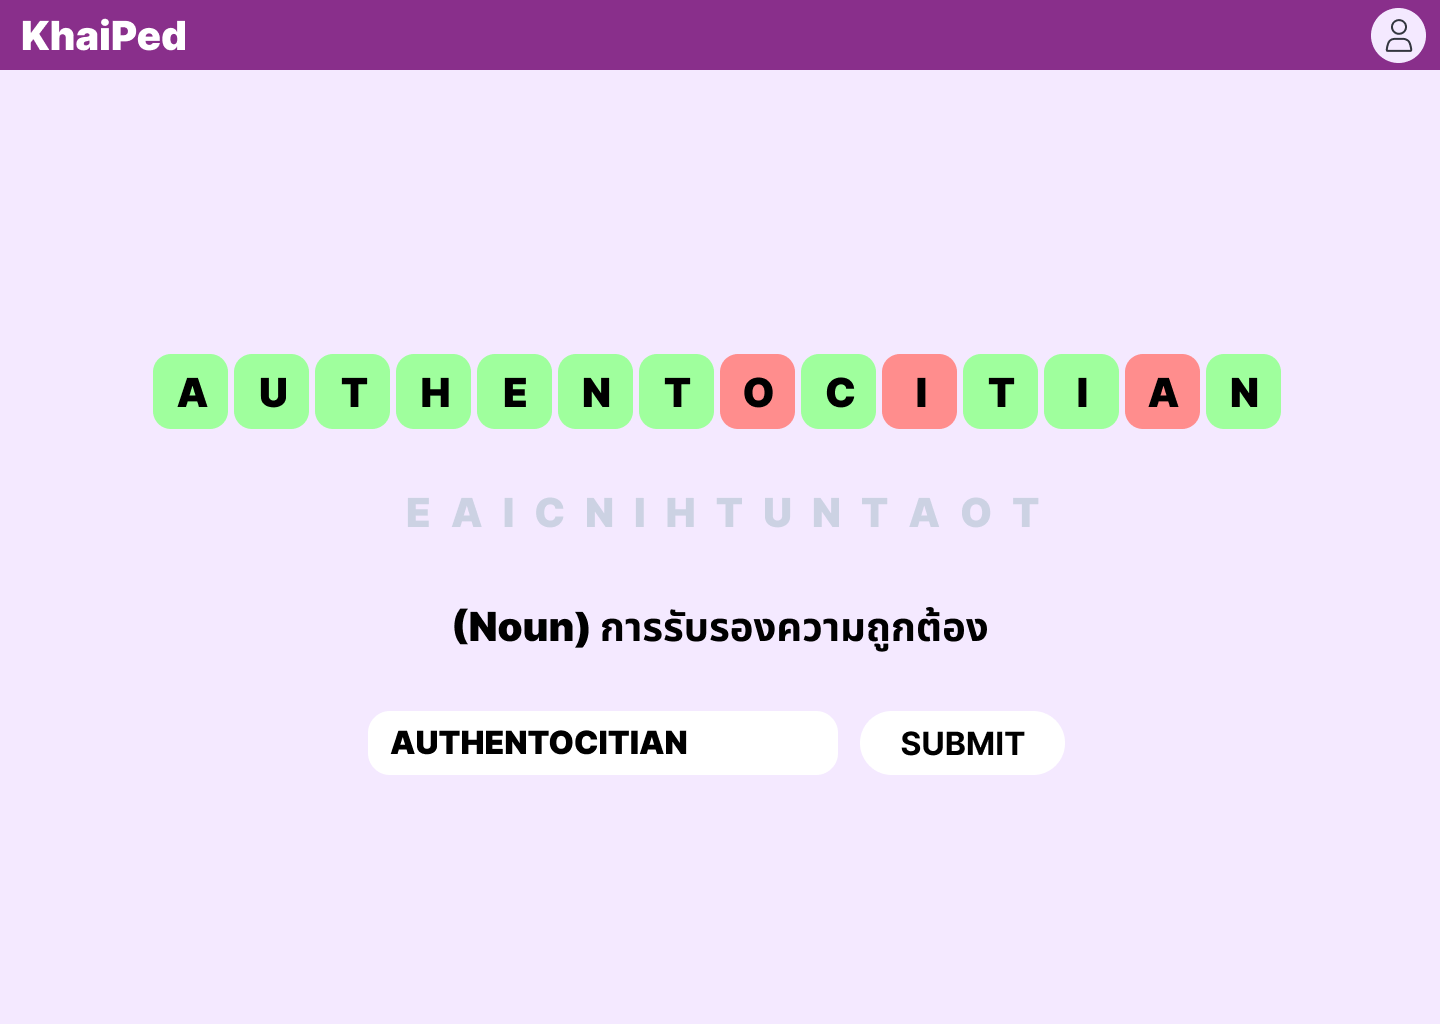
\includegraphics[width=0.8\textwidth, keepaspectratio=true]{image/chap3/ui/game/Word Scramble - Wrong Answer.png}
	\caption{การแสดงผลหากใส่คำตอบผิด}\label{fig:UI_GameWrong}
\end{figure}
\hspace{1cm}
หากผู้ใช้ใส่พยัญชนะผิดตำแหน่งและกดปุ่มส่งคำศัพท์ ระบบจะตรวจสอบว่าตัวอักษรที่ผู้ใช้ใส่ถูกตำแหน่งหรือไม่ และจะแสดงผลพยัญชนะที่อยู่ในตำแหน่งถูก และผิด

\pagebreak
\begin{figure}[!h]\centering
	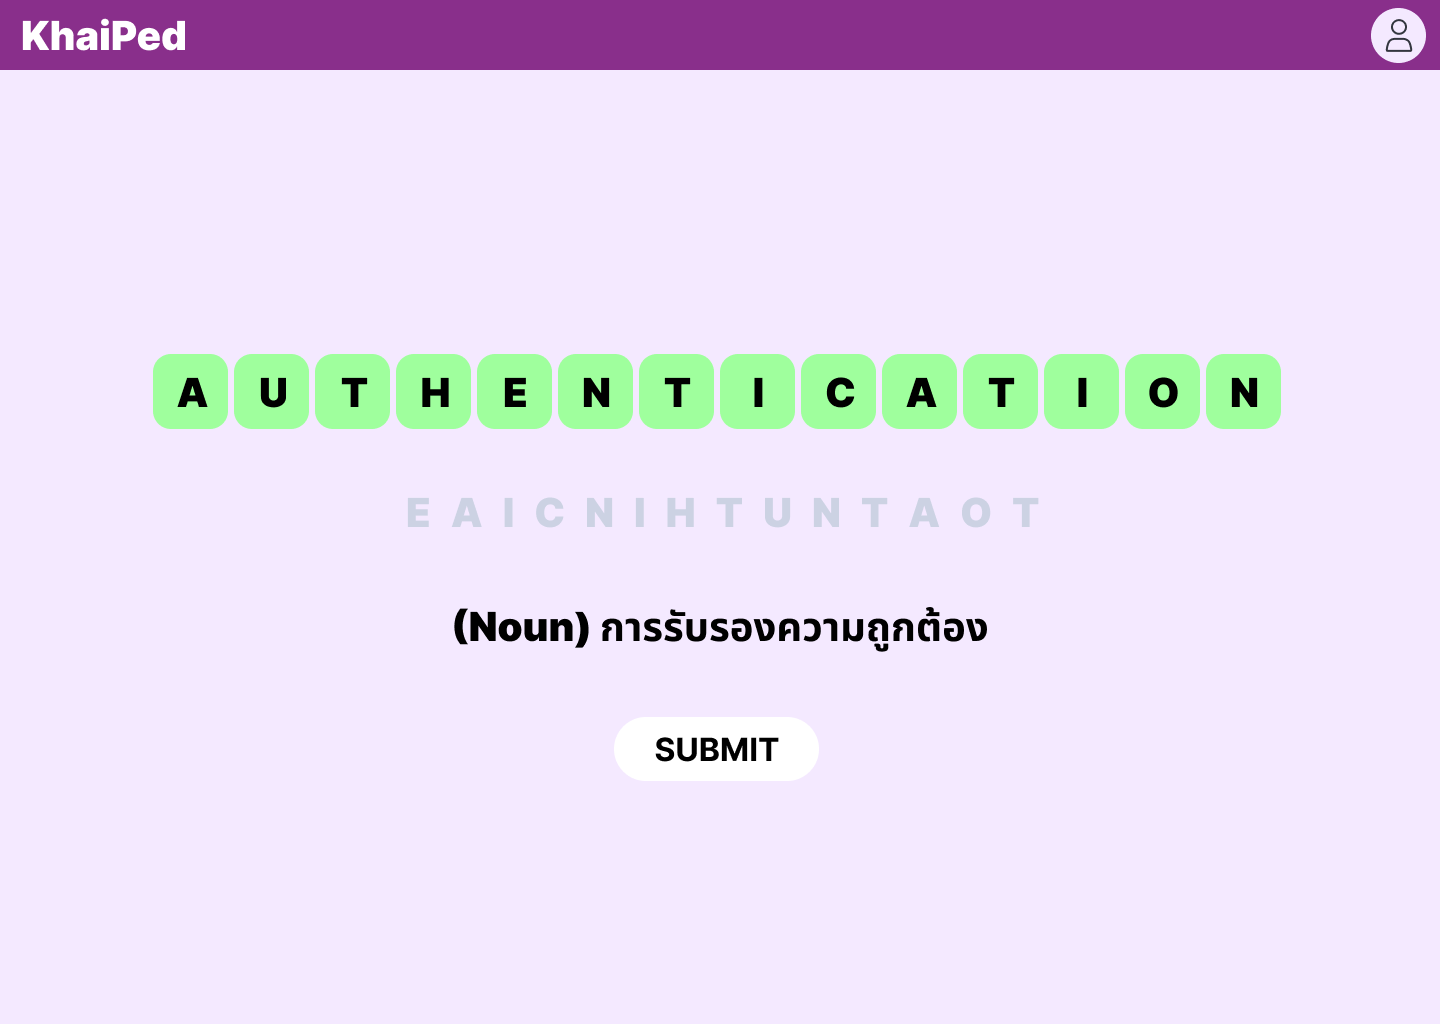
\includegraphics[width=0.8\textwidth, keepaspectratio=true]{image/chap3/ui/game/Word Scramble - Correct Answer.png}
	\caption{การแสดงผลหากใส่คำตอบถูก}\label{fig:UI_GameCorrect}
\end{figure}
\hspace{1cm}
หากผู้ใช้ใส่พยัญชนะถูกทุกตำแหน่งและกดปุ่มส่งคำศัพท์ ระบบจะตรวจสอบว่าตัวอักษรที่ผู้ใช้ใส่ถูกตำแหน่งหรือไม่ และจะแสดงผลพยัญชนะที่อยู่ในตำแหน่งถูก 

\begin{figure}[!h]\centering
	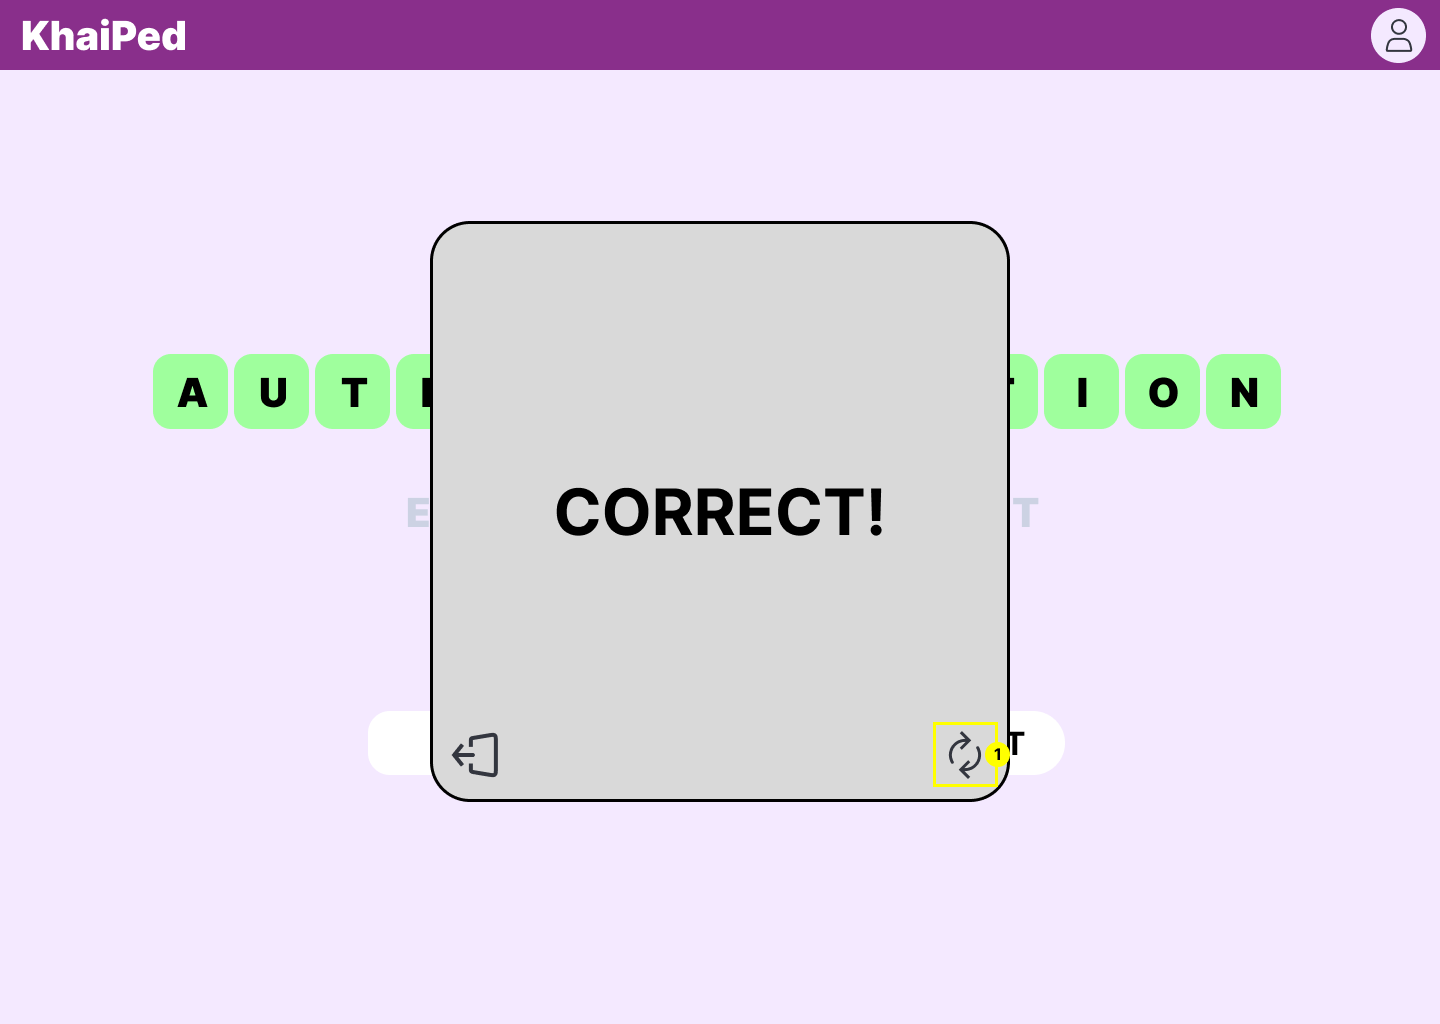
\includegraphics[width=0.8\textwidth, keepaspectratio=true]{image/chap3/ui/game/Word Scramble - Pop Up.png}
	\caption{การแสดงผลลัพท์การเล่นเกม}\label{fig:UI_GameResult}
\end{figure}
\hspace{1cm}
เมื่อผู้ใช้เรียงคำศัพท์ได้ถูกต้องแล้วกดปุ่มส่งคำศัพท์ หลังจากที่ระบบแสดงผลพยัญชนะที่อยู่ในตำแหน่งถูกแล้ว ระบบจะแสดงผลว่าผู้ใช้เรียงคำศัพท์ได้ถูกต้อง
และสามารถกดปุ่มออกเพื่อกลับไปหน้าหลัก หรือกดปุ่มสุ่มคำใหม่ เพื่อให้ระบบจะสุ่มคำศัพท์ใหม่มาเล่นเกมต่อได้

\pagebreak
\begin{figure}[!h]\centering
	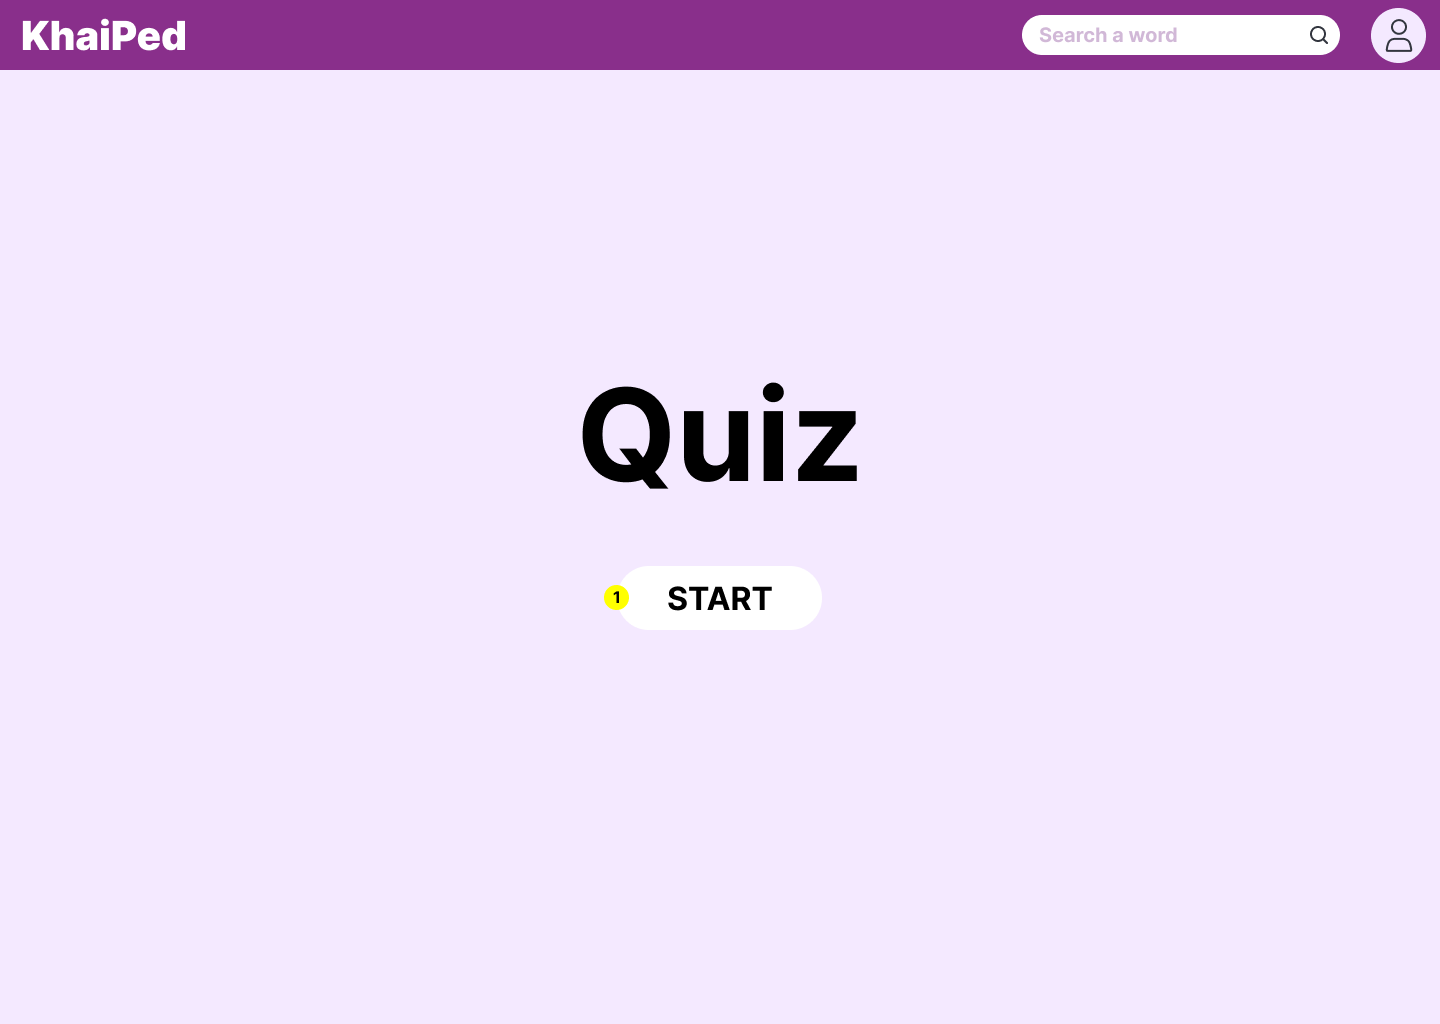
\includegraphics[width=0.8\textwidth, keepaspectratio=true]{image/chap3/ui/quiz/Quiz.png}
	\caption{หน้าหลักการทำแบบทดสอบ}\label{fig:UI_Quiz}
\end{figure}
\hspace{1cm}
เมื่อผู้ใช้กดปุ่มทำแบบทดสอบในหน้าหลัก ระบบจะแสดงผลหน้าเล่นเกมโดยในหน้าจะประกอบไปด้วยปุ่มเริ่มทำแบบทดสอบ (1) เมื่อกดแล้ว ระบบจะทำการสุ่มคำศัพท์ 10 คำและแสดงผลหน้าสำหรับทำแบบทดสอบ

\begin{figure}[!h]\centering
	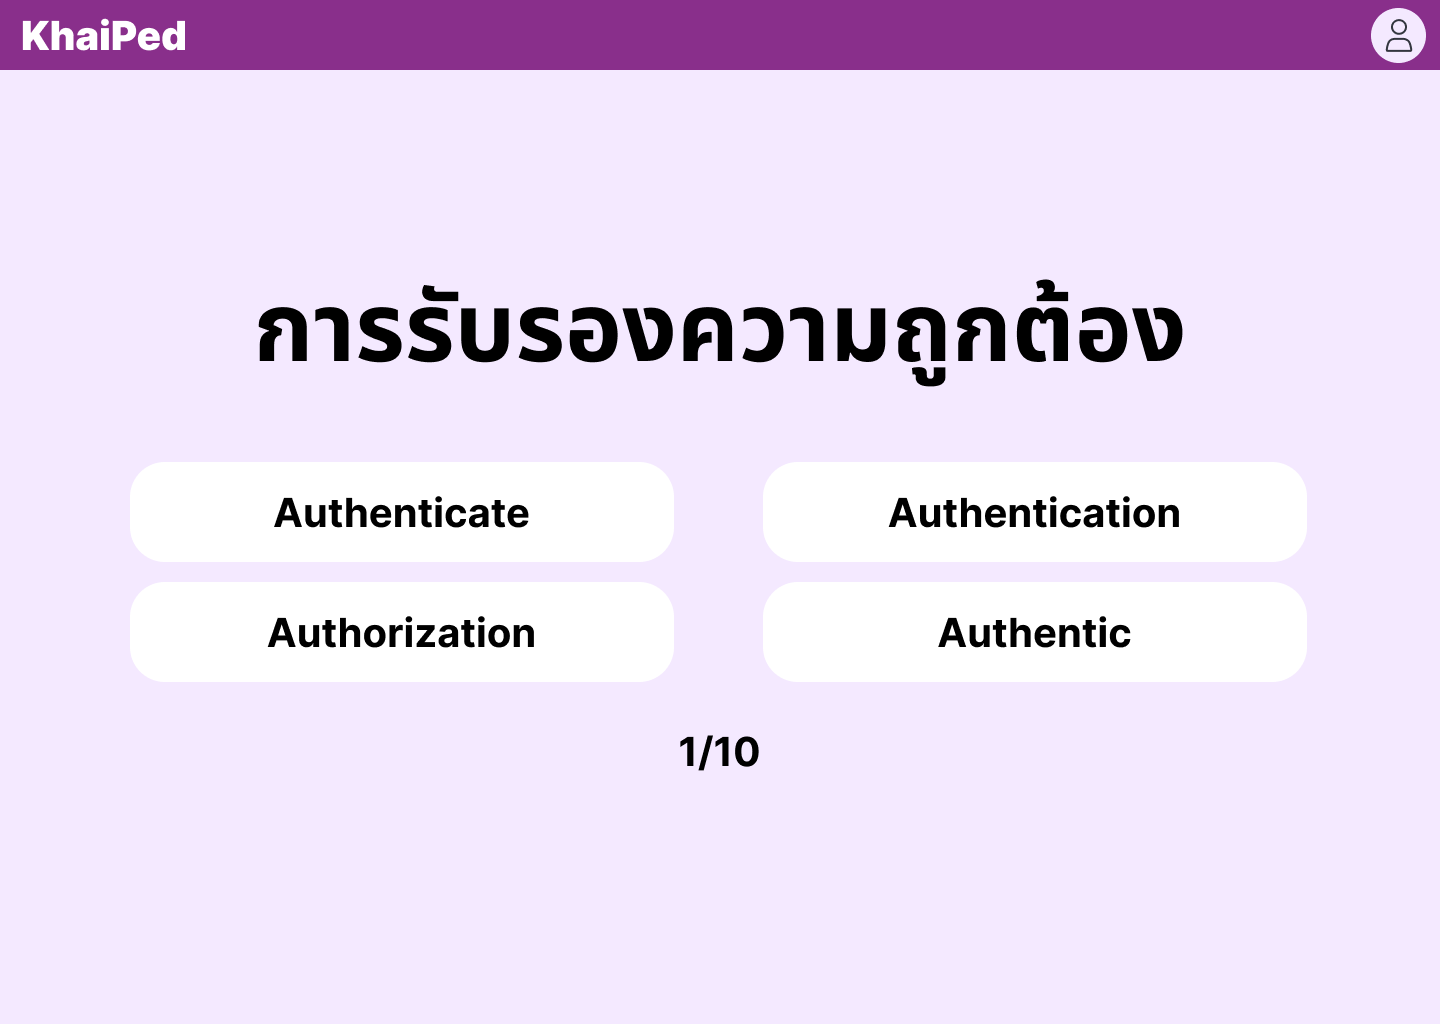
\includegraphics[width=0.8\textwidth, keepaspectratio=true]{image/chap3/ui/quiz/Quiz - Start.png}
	\caption{หน้าเริ่มการทำแบบทดสอบ}\label{fig:UI_QuizStart}
\end{figure}
\hspace{1cm}
เมื่อผู้ใช้กดปุ่มเริ่มทำแบบทดสอบแล้ว ระบบจะแสดงผลหน้าสำหรับทำแบบทดสอบ โดยจะประกอบไปด้วยโจทย์ ตัวเลือก 4 ข้อ และจำนวนข้อที่เหลืออยู่

\pagebreak
\begin{figure}[!h]\centering
	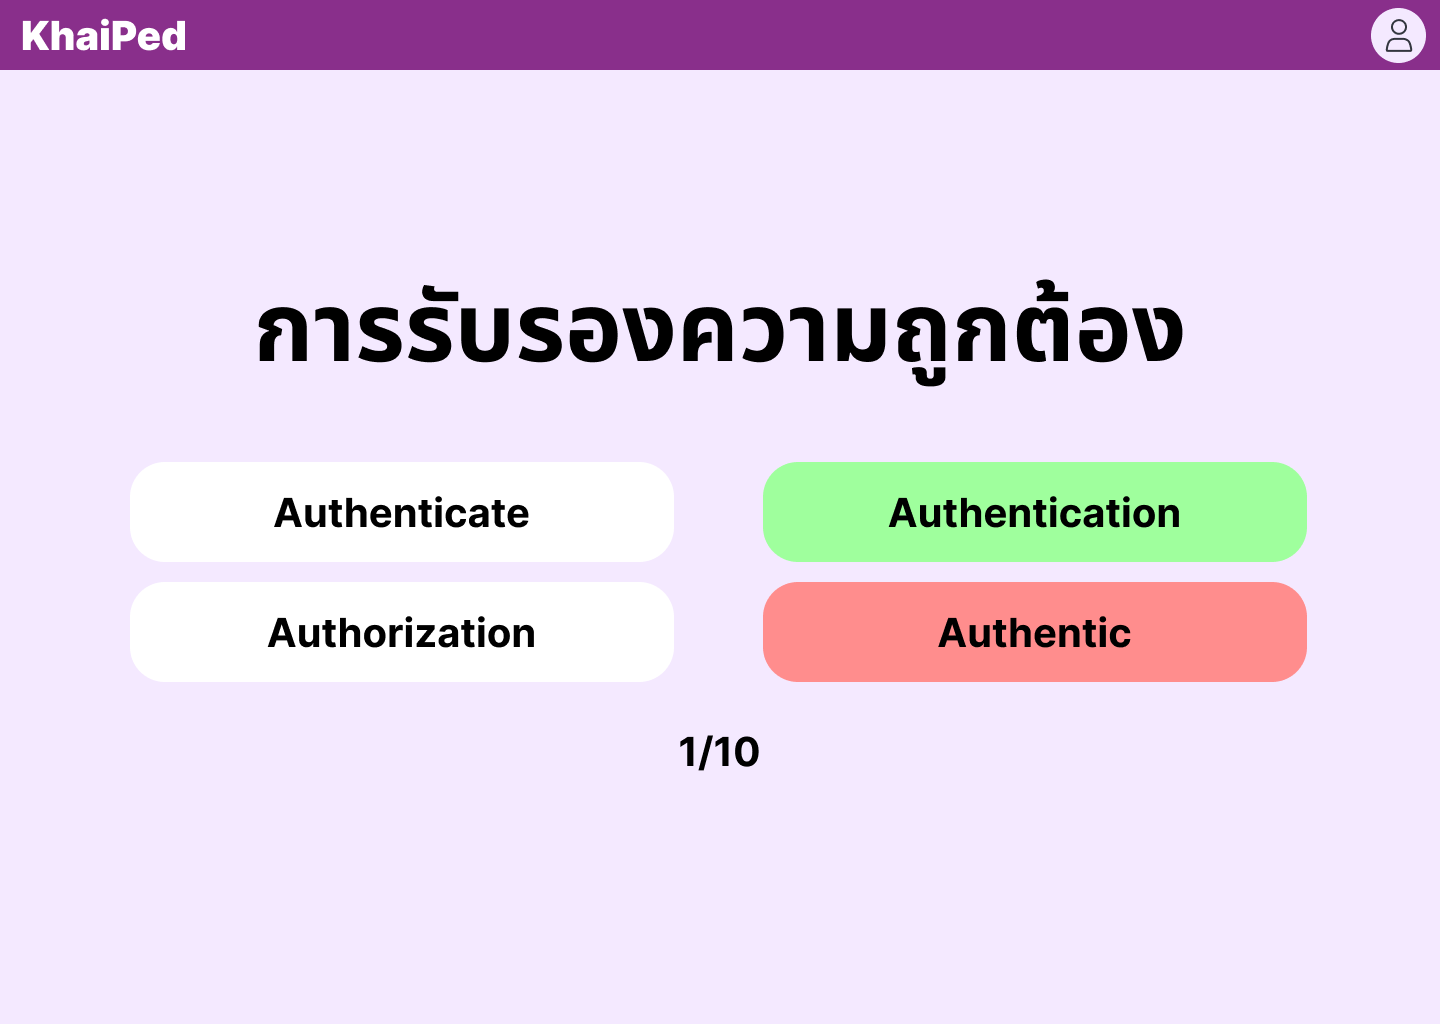
\includegraphics[width=0.8\textwidth, keepaspectratio=true]{image/chap3/ui/quiz/Quiz - Wrong Answer.png}
	\caption{การแสดงผลหากตอบผิด}\label{fig:UI_QuizWrong}
\end{figure}
\hspace{1cm}
หากผู้ใช้เลือกคำตอบผิด ระบบจะแสดงว่าคำตอบที่เลือกผิดโดยขึ้นเป็นสีแดง แล้วแสดงคำตอบที่ถูกเป็นสีเขียว จากนั้นจะแสดงผลข้อถัดไป

\begin{figure}[!h]\centering
	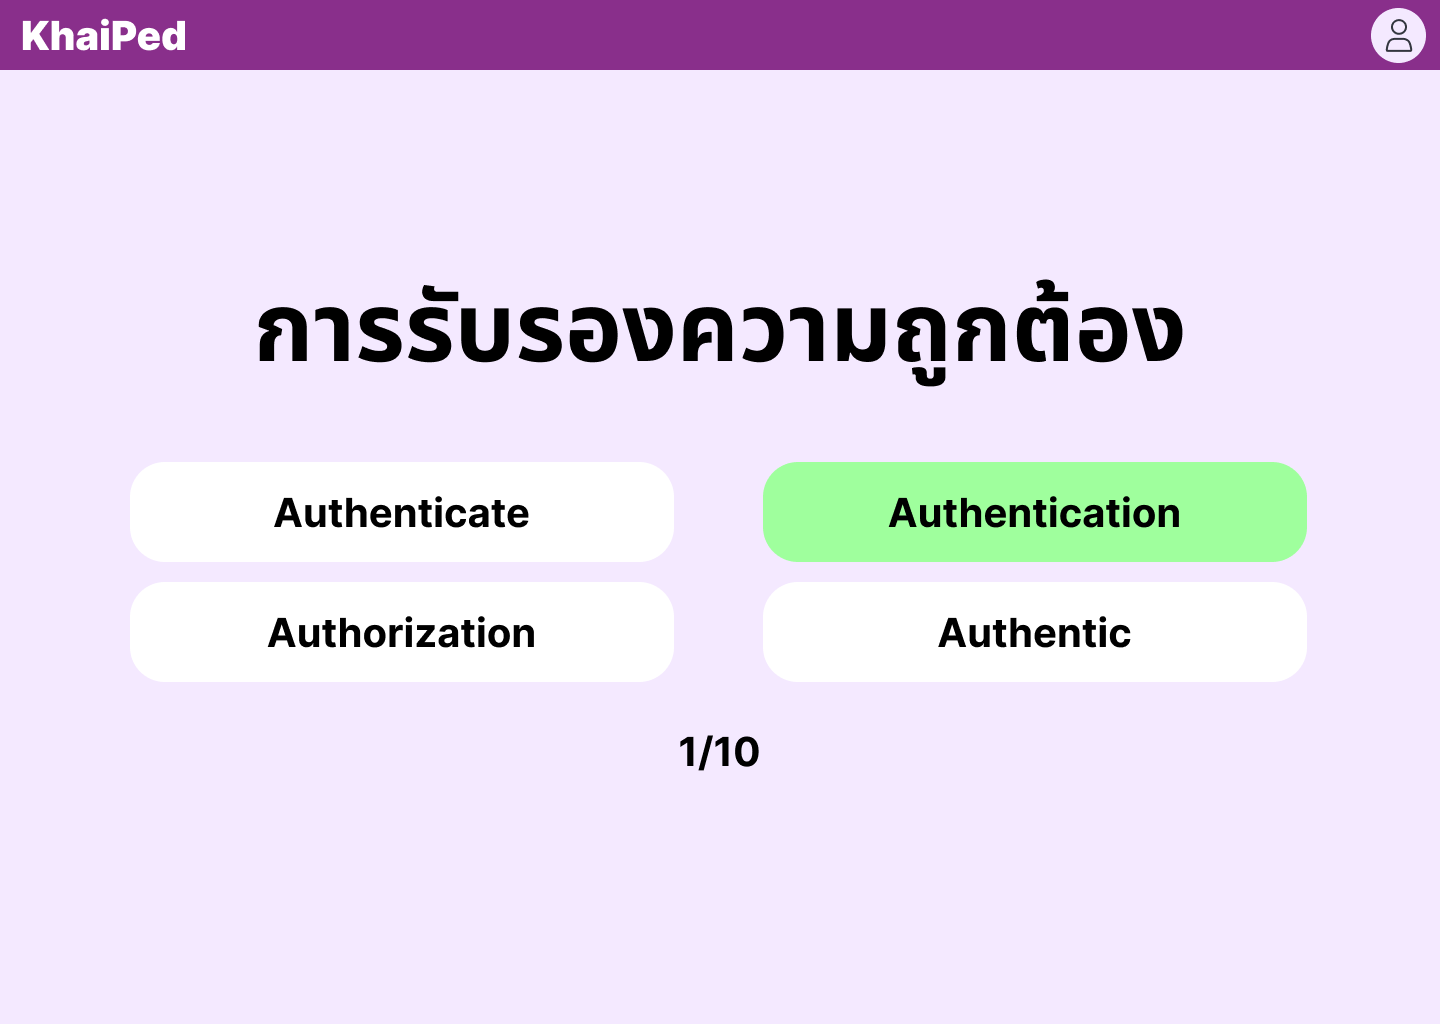
\includegraphics[width=0.8\textwidth, keepaspectratio=true]{image/chap3/ui/quiz/Quiz - Correct Answer.png}
	\caption{การแสดงผลหากตอบถูก}\label{fig:UI_QuizCorrect}
\end{figure}
\hspace{1cm}
หากผู้ใช้เลือกคำตอบถูก ระบบจะแสดงว่าคำตอบที่เลือกถูกเป็นสีเขียว จากนั้นจะแสดงผลข้อถัดไป

\pagebreak
\begin{figure}[!h]\centering
	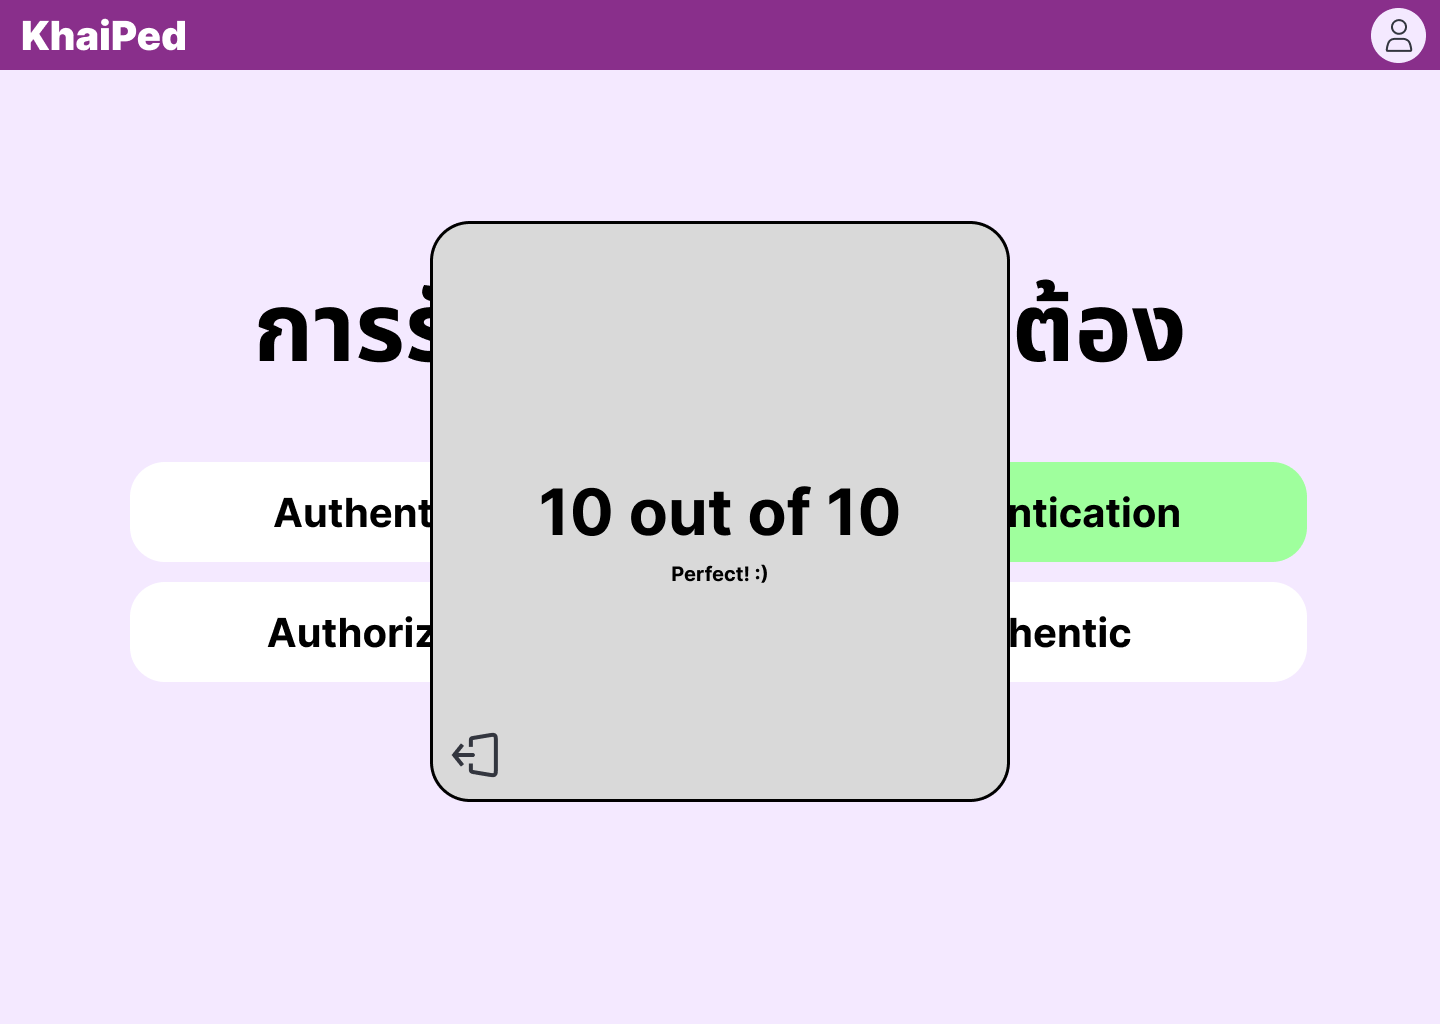
\includegraphics[width=0.8\textwidth, keepaspectratio=true]{image/chap3/ui/quiz/Quiz - Result.png}
	\caption{การแสดงผลลัพท์การทำแบบทดสอบ}\label{fig:UI_QuizResult}
\end{figure}
\hspace{1cm}
หากผู้ใช้ตอบคำถามครบ 10 ข้อแล้ว ระบบจะแสดงคำตอบของข้อนั้น ๆ แล้วแจ้งเตือนคะแนนที่ผู้ใช้ทำได้ และผู้ใช้สามารถกดปุ่มออกเพื่อกลับไปหน้าหลักได้

\begin{figure}[!h]\centering
	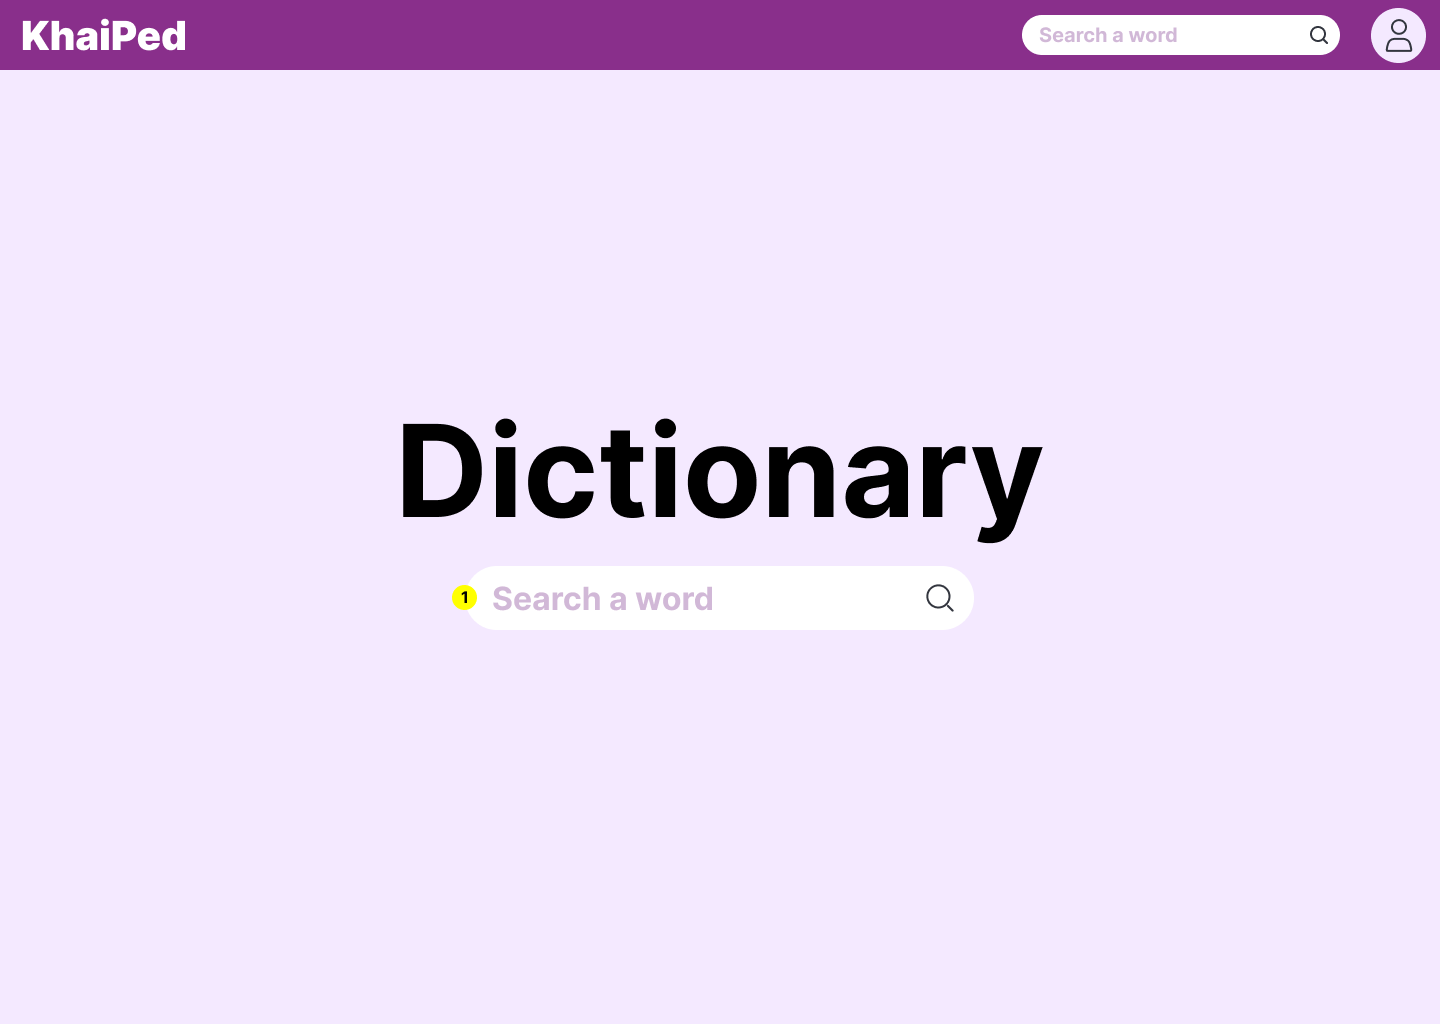
\includegraphics[width=0.8\textwidth, keepaspectratio=true]{image/chap3/ui/dict/Dictionary.png}
	\caption{หน้าหลักพจนานุกรม}\label{fig:UI_Dictionary}
\end{figure}
\hspace{1cm}
เมื่อผู้ใช้กดปุ่มพจนานุกรมในหน้าหลัก ระบบจะแสดงผลหน้าพจนานุกรมโดยในหน้าจะประกอบไปด้วยช่องค้นหา (1) เมื่อค้นหาแล้ว ระบบจะทำการค้นหาคำศัพท์ในฐานข้อมูลแล้วทำการแสดงผล

\pagebreak
\begin{figure}[!h]\centering
	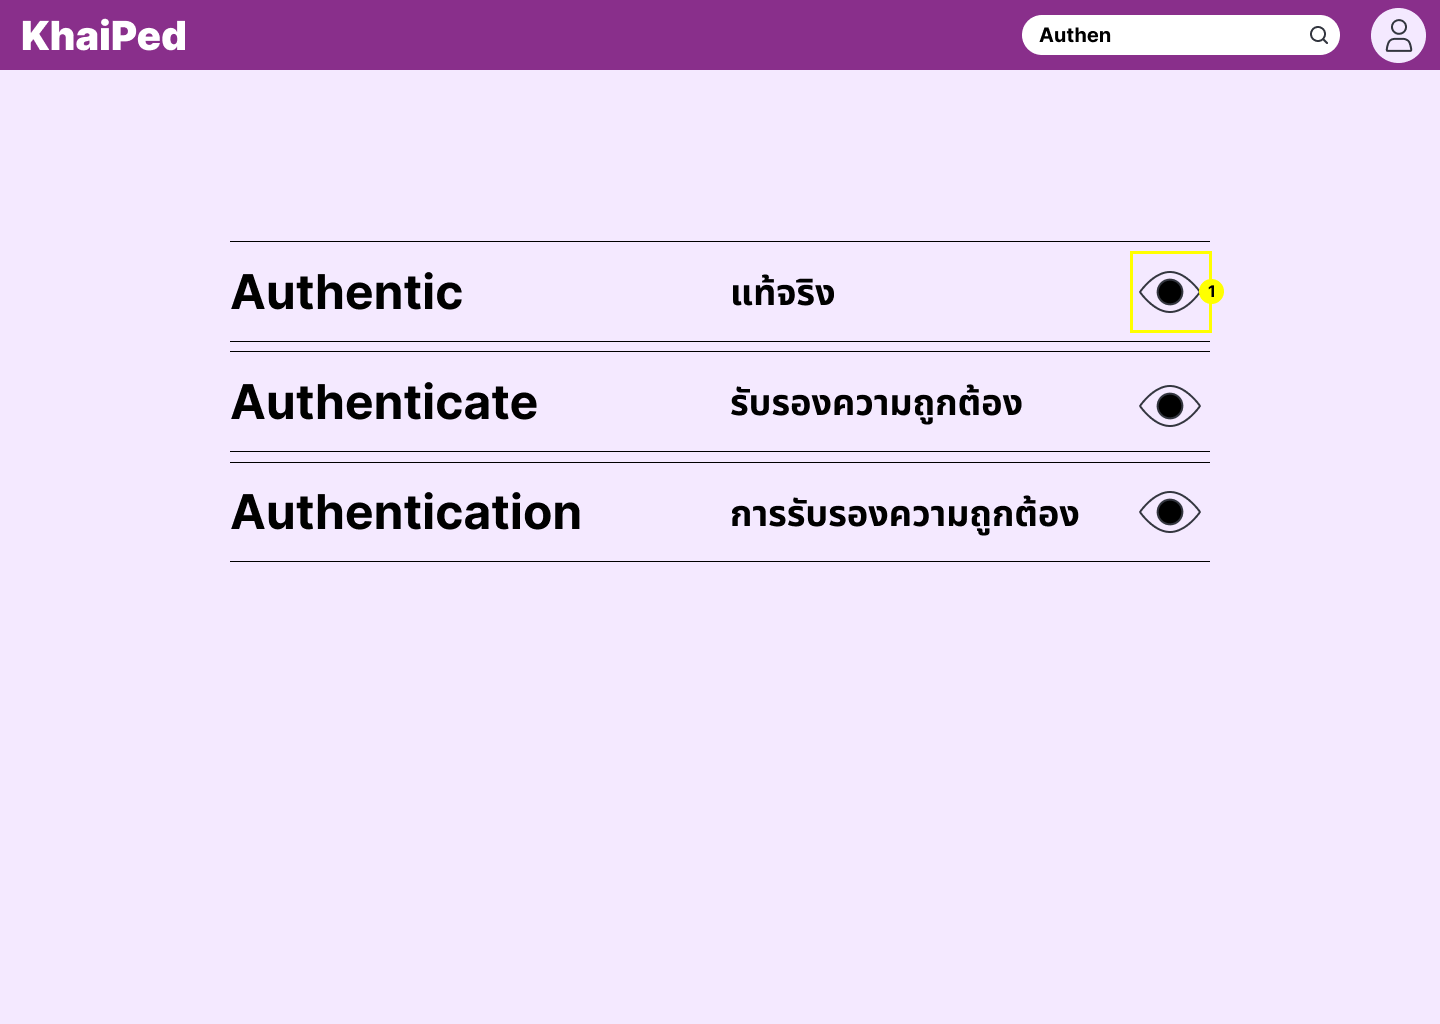
\includegraphics[width=0.8\textwidth, keepaspectratio=true]{image/chap3/ui/dict/Dictionary - Search Word.png}
	\caption{หน้าแสดงผลการค้นหา}\label{fig:UI_DictionarySearch}
\end{figure}
\hspace{1cm}
เมื่อผู้ใช้ค้นหาคำศัพท์จากช่องค้นหา หรือในหน้าพจนานุกรม ระบบจะแสดงผลการ์ดคำศัพท์ที่ทำการค้นหาออกมา โดยจะสามารถกดปุ่มดูรายละเอียด (1) เพื่อดูรายละเอียดคำศัพท์นั้น ๆ ได้

\begin{figure}[!h]\centering
	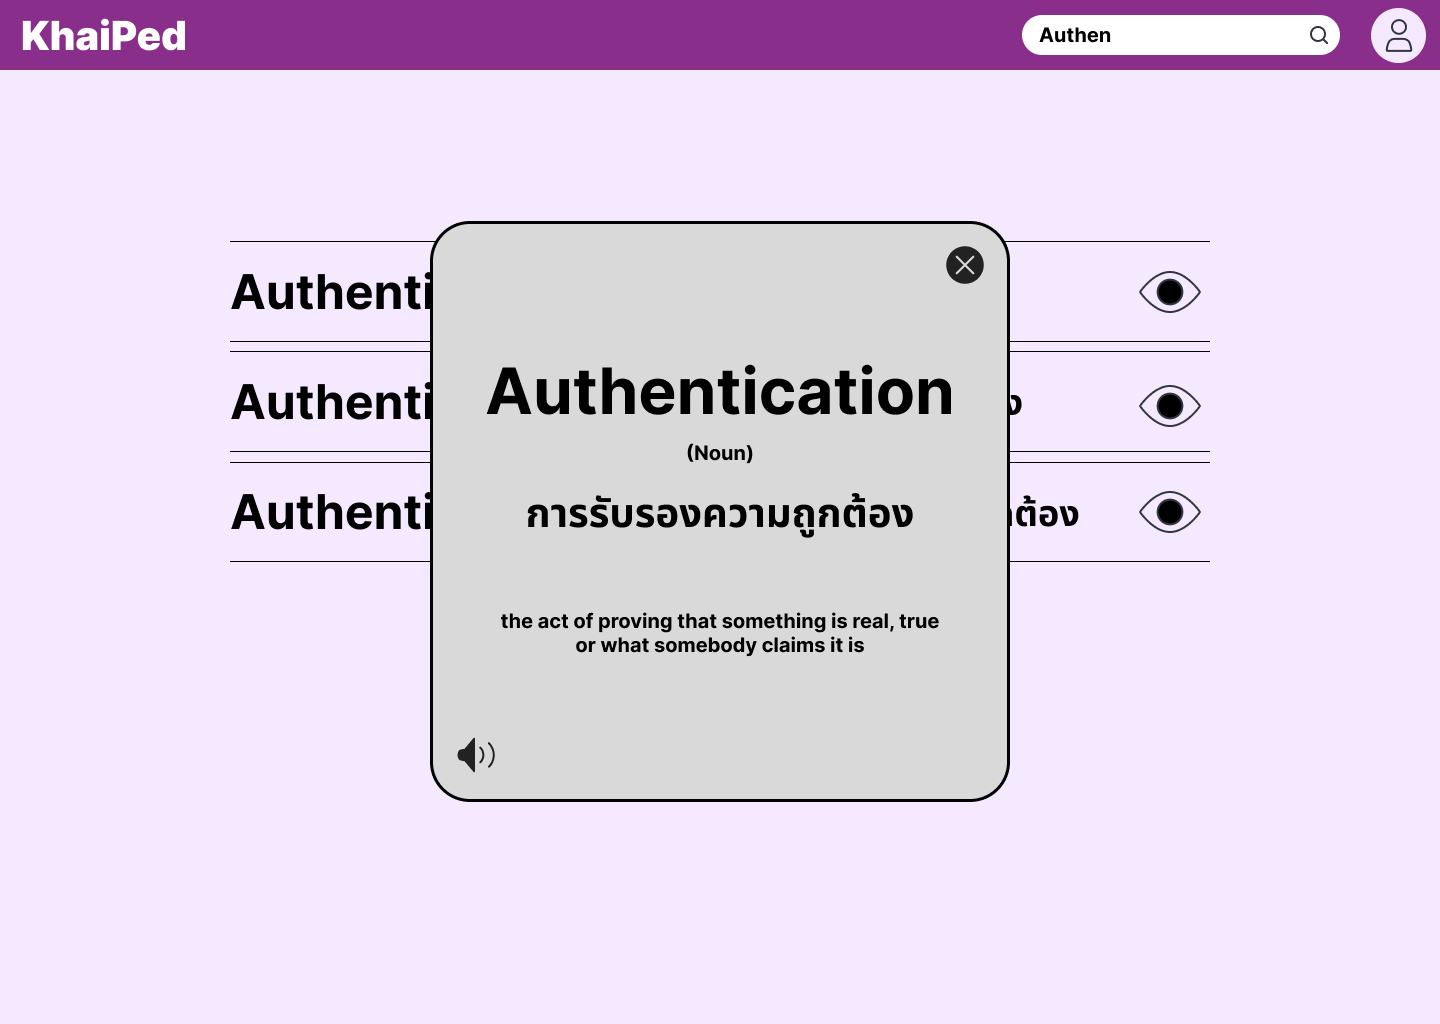
\includegraphics[width=0.8\textwidth, keepaspectratio=true]{image/chap3/ui/dict/Dictionary - View Word.png}
	\caption{การแสดงผลรายละเอียดคำศัพท์}\label{fig:UI_DictionaryView}
\end{figure}
\hspace{1cm}
เมื่อผู้ใช้กดปุ่มแสดงรายละเอียด ระบบจะแสดงผลรายละเอียดของคำนั้น ๆ โดยสามารถกดปุ่มปิด หรือกดปุ่มเล่นเสียงที่เล่นเสียงวิธีการออกเสียงของคำศัพท์ได้

%%%%%%%%%%%%%%%%%%%%%%%%%%%%%%%%%%%%%%%%%%%%%%%%%%%%%%%%%%%%%%%%
%%%%%%%%%%%%%%%%%%%%%%%%% Bibliography %%%%%%%%%%%%%%%%%%%%%%%%%
%%%%%%%%%%%%%%%%%%%%%%%%%%%%%%%%%%%%%%%%%%%%%%%%%%%%%%%%%%%%%%%%

%%%% Comment this in your report to show only references you have
%%%% cited. Otherwise, all the references below will be shown.
%\nocite{*}
%% Use the kmutt.bst for bibtex bibliography style 
%% You must have cpe.bib and string.bib in your current directory.
%% You may go to file .bbl to manually edit the bib items.

% Sept, 2021 by Thanin
% improve url breaks to prevent unnecessary big white spaces in some cases
\makeatletter
\g@addto@macro{\UrlBreaks}{\UrlOrds}
\makeatother
% 

\bibliographystyle{kmutt}
\bibliography{string,cpe}

\end{document}